% ===========================================================================
% 模式识别课程设计说明书
% 基于深度学习的胸片肺炎二分类与跨来源域偏移研究
% 硕士毕业论文格式标准
% ===========================================================================

\documentclass[12pt,a4paper,UTF8,openany]{ctexbook}

% ======================== 页面设置 ========================
\usepackage[top=2.54cm, bottom=2.54cm, left=3.17cm, right=3.17cm, headheight=18pt]{geometry}
\usepackage{setspace}
\onehalfspacing
\usepackage{microtype}
\setlength{\emergencystretch}{2.5em}
\tolerance=1800
\hbadness=1800
\widowpenalty=10000
\clubpenalty=10000
\displaywidowpenalty=10000

% ======================== 字体与编码 ========================
\usepackage{fontspec}
\setmainfont{Times New Roman}
\setCJKmainfont{SimSun}[AutoFakeBold=2.5]
\setCJKsansfont{SimHei}[AutoFakeBold=2.5]
\setCJKmonofont{KaiTi}[AutoFakeBold=2.5]

% xeCJK 全局伪粗体：从 xeCJK 层面处理 CJK 粗体，避免 fontspec NFSS 警告
\xeCJKsetup{AutoFakeBold=true, EmboldenFactor=2.5}

% 静默 SimHei 无粗体变体的 fontspec 警告（xeCJK 的 AutoFakeBold 已在上层处理）
\usepackage{silence}
\WarningFilter{latexfont}{Font shape `TU/SimHei(0)/b/n' undefined}
\WarningFilter{latexfont}{Some font shapes}

% ======================== 图表与公式 ========================
\usepackage{amsmath, amssymb, amsthm}
\usepackage{graphicx}
\usepackage{float}
\usepackage{booktabs}
\usepackage{multirow}
\usepackage{longtable}
\usepackage{array}
\usepackage{tabularx}
\usepackage{adjustbox}
\usepackage{caption}
\usepackage{subcaption}
\captionsetup{font=small, labelfont=bf, justification=centering, singlelinecheck=false, skip=6pt}
\setlength{\textfloatsep}{14pt plus 3pt minus 2pt}
\setlength{\floatsep}{12pt plus 3pt minus 2pt}
\setlength{\intextsep}{12pt plus 3pt minus 2pt}
\renewcommand{\topfraction}{0.88}
\renewcommand{\bottomfraction}{0.75}
\renewcommand{\textfraction}{0.10}
\renewcommand{\floatpagefraction}{0.78}
\setcounter{topnumber}{3}
\setcounter{bottomnumber}{2}
\setcounter{totalnumber}{4}
\usepackage[section]{placeins}

% ======================== 超链接与引用 ========================
\usepackage[colorlinks=true, linkcolor=black, citecolor=black, urlcolor=blue]{hyperref}
\usepackage{url}
\usepackage{xurl}
\usepackage[htt]{hyphenat}

% ======================== 页眉页脚 ========================
\usepackage{fancyhdr}
\pagestyle{fancy}
\fancyhf{}
\fancyhead[R]{\leftmark}
\fancyfoot[C]{\thepage}
\renewcommand{\headrulewidth}{0.4pt}

% ======================== 章节标题格式 ========================
\ctexset{
  chapter={
    name={第,章},
    number=\arabic{chapter},
    format={\centering\heiti\zihao{3}},
    aftername={\quad},
    beforeskip={20pt},
    afterskip={20pt},
  },
  section={
    format={\heiti\zihao{4}},
    beforeskip={12pt},
    afterskip={8pt},
  },
  subsection={
    format={\heiti\zihao{-4}},
    beforeskip={8pt},
    afterskip={6pt},
  },
}

% ======================== 目录设置 ========================
\usepackage{tocloft}
\renewcommand{\cfttoctitlefont}{\heiti\zihao{3}\bfseries}
\renewcommand{\cftchapfont}{\heiti\bfseries}
\renewcommand{\cftsecfont}{\songti}
\renewcommand{\cftchappagefont}{\normalfont}
\renewcommand{\cftsecpagefont}{\normalfont}
\setlength{\cftbeforechapskip}{6pt}

% ======================== 列表环境 ========================
\usepackage{enumitem}
\setlist{nosep, leftmargin=2em}

% ======================== 代码环境 ========================
\usepackage{listings}
\usepackage{xcolor}
\lstset{
  basicstyle=\footnotesize\ttfamily,
  breaklines=true,
  breakatwhitespace=false,
  columns=fullflexible,
  keepspaces=true,
  postbreak=\mbox{\textcolor{gray}{$\hookrightarrow$}\space},
  frame=single,
  numbers=left,
  numberstyle=\tiny,
  commentstyle=\color{gray},
  keywordstyle=\color{blue},
  stringstyle=\color{red},
  showstringspaces=false,
  literate={≈}{{$\approx$}}1,
  tabsize=4,
  language=Python,
  aboveskip=8pt,
  belowskip=8pt,
  xleftmargin=1.2em,
  framexleftmargin=0.8em,
}

% ======================== 参考文献 ========================
% 使用 natbib 数字引用格式，兼容 GB/T 7714 顺序编码制
\usepackage[numbers,sort&compress,square]{natbib}
\setcitestyle{numbers,square}

% ======================== 摘要环境 ========================
\newenvironment{cnabstract}{
  \chapter*{\centering\heiti\zihao{3} 摘\quad 要}
  \addcontentsline{toc}{chapter}{摘要}
  \thispagestyle{plain}
  \setlength{\parindent}{2em}
}{
  \par\vspace{2em}
  \noindent{\heiti 关键词：}胸片；肺炎分类；域偏移；跨来源评估；概率校准
}

\newenvironment{enabstract}{
  \chapter*{\centering\bfseries\zihao{3} Abstract}
  \addcontentsline{toc}{chapter}{Abstract}
  \thispagestyle{plain}
  \setlength{\parindent}{0em}
}{
  \par\vspace{2em}
  \noindent{\bfseries Keywords: }Chest X-ray; Pneumonia Classification; Domain Shift; Cross-source Evaluation; Probability Calibration
}

% ======================== 文档开始 ========================
\begin{document}
\let\cleardoublepage\clearpage

% ======================== 封面 ========================
\begin{titlepage}
  \thispagestyle{empty}
  \begin{center}
    \vspace*{0.35cm}
    \begin{minipage}{0.78\textwidth}
      \centering
      
\includegraphics[width=2.35cm]{figures/cover_emblem.png}\hspace{0.55cm}%
      \raisebox{0.55cm}{
\includegraphics[width=8.0cm]{figures/cover_wordmark.png}}
    \end{minipage}

    \vspace{1.55cm}
    {\songti\zihao{1} 模式识别与机器学习课程设计报告\par}

    \vspace{1.85cm}
    {\songti\zihao{3}%
      \makebox[\textwidth][c]{题\quad 目：\hspace{0.55cm}选题 78——肺炎 X 光图像诊断识别}\par
    }

    \vfill
    \begin{minipage}{11.8cm}
      \songti\zihao{-3}
      \setlength{\parindent}{0pt}
      \setlength{\parskip}{0pt}
      \makebox[11.8cm][c]{\makebox[2.2cm][s]{院系}\hspace{0.35cm}\underline{\makebox[8.05cm]{人工智能与自动化学院}}}\par\vspace{0.32cm}
      \makebox[11.8cm][c]{\makebox[2.2cm][s]{专业班级}\hspace{0.35cm}\underline{\makebox[8.05cm]{自动化（卓越）2301 班}}}\par\vspace{0.32cm}
      \makebox[11.8cm][c]{\makebox[2.2cm][s]{指导老师}\hspace{0.35cm}\underline{\makebox[8.05cm]{程\quad 骋}}}\par

      \vspace{0.72cm}
      \makebox[11.8cm][c]{\makebox[1.65cm][s]{姓名}\hspace{0.25cm}\underline{\makebox[3.05cm]{张龙骥}}\hspace{0.70cm}\makebox[1.65cm][s]{学号}\hspace{0.25cm}\underline{\makebox[3.05cm]{U202315182}}}\par\vspace{0.34cm}
      \makebox[11.8cm][c]{\makebox[1.65cm][s]{姓名}\hspace{0.25cm}\underline{\makebox[3.05cm]{高金泽}}\hspace{0.70cm}\makebox[1.65cm][s]{学号}\hspace{0.25cm}\underline{\makebox[3.05cm]{U202315082}}}\par\vspace{0.34cm}
      \makebox[11.8cm][c]{\makebox[1.65cm][s]{姓名}\hspace{0.25cm}\underline{\makebox[3.05cm]{蔡沐河}}\hspace{0.70cm}\makebox[1.65cm][s]{学号}\hspace{0.25cm}\underline{\makebox[3.05cm]{U202310165}}}\par\vspace{0.34cm}
      \makebox[11.8cm][c]{\makebox[1.65cm][s]{姓名}\hspace{0.25cm}\underline{\makebox[3.05cm]{李际宏}}\hspace{0.70cm}\makebox[1.65cm][s]{学号}\hspace{0.25cm}\underline{\makebox[3.05cm]{U202312011}}}\par\vspace{0.34cm}
      \makebox[11.8cm][c]{\makebox[1.65cm][s]{姓名}\hspace{0.25cm}\underline{\makebox[3.05cm]{张文博}}\hspace{0.70cm}\makebox[1.65cm][s]{学号}\hspace{0.25cm}\underline{\makebox[3.05cm]{U202314552}}}\par
    \end{minipage}
    \vspace{1.25cm}
  \end{center}
\end{titlepage}
\iffalse
\begin{titlepage}
  \thispagestyle{empty}
  \vspace*{1.0cm}

  \begin{center}
    {\heiti\zihao{-0}\bfseries 课程设计说明书}

    \vspace{2.0cm}

    \begin{minipage}{0.90\textwidth}
      \centering
      {\heiti\zihao{2}\bfseries 基于深度学习的胸片肺炎二分类\\[0.25cm]
      与跨来源域偏移研究}
    \end{minipage}

    \vspace{0.55cm}

    {\bfseries\zihao{3} Deep Learning-Based Chest X-Ray Pneumonia Binary\\
      Classification and Cross-Source Domain Shift Study}

    \vspace{2.0cm}

    \begin{large}
      \begin{tabular}{rl}
        {\heiti 指导教师：} & \underline{\makebox[5cm]{程骋}} \\[0.4cm]
        {\heiti 课程名称：} & \underline{\makebox[5cm]{模式识别与机器学习课程设计}} \\[0.4cm]
        {\heiti 所属院系：} & \underline{\makebox[5cm]{人工智能与自动化学院}} \\[0.4cm]
        {\heiti 提交日期：} & \underline{\makebox[5cm]{\today}} \\[0.4cm]
      \end{tabular}
    \end{large}

  \end{center}
\end{titlepage}
\fi

% ======================== 前言设置 ========================
\frontmatter
\pagenumbering{Roman}

% ======================== 中文摘要 ========================
\begin{cnabstract}

胸片（Chest X-ray, CXR）是肺炎诊断中最常用的影像学检查手段。近年来，深度学习在医学影像分类中取得了很好的效果，但一个问题仍然没有很好的答案：在一个公开数据集上表现优异的模型，换成另一个来源的数据后，性能还能保持吗？本课程设计围绕这个跨来源域偏移（Domain Shift）问题，使用 PyTorch 框架实现了 DenseNet121、ConvNeXt-Tiny 和 Vision Transformer (ViT-B/16) 三种深度学习模型，并设计了经验风险最小化（ERM）、正则化增强训练（ERM-Reg）、联合训练（JT）和域均衡采样联合训练（JT-DBS）四种训练方案，在 Kermany 儿科胸片数据集和 RSNA 肺炎检测挑战赛数据集上共完成了 18 次训练和双数据集评估。

实验发现，三种模型在源域 Kermany 测试集上的平衡准确率都超过了 97\%，但在跨来源的 RSNA 子集上只达到约 66\%，特异度最低只有 0.35，大量正常图像被误判为肺炎。将两个数据集混合训练后，DenseNet121 在 RSNA 上的集成平衡准确率从 0.6591 提高到了 0.7813，但召回率从 0.9648 降到了 0.7533，整体指标变好了，但漏诊变多了。来源可分性分析还显示，在控制类别比例、排除宽高比后，仅凭均值、标准差等十个简单的像素统计特征就能以 0.944 的 AUROC 区分图像来自哪个数据集，说明两个数据集在底层图像特征上确实存在不小的差异。

本课程设计覆盖了数据审计、模型训练、校准分析和统计检验，代码与配置随仓库保存。结果提示，单一数据来源上的高分不能直接代表跨来源可用性，医学影像模型需要在独立来源上接受检验。

\end{cnabstract}

% ======================== 英文摘要 ========================
\begin{enabstract}

Chest X-ray (CXR) is the most commonly used first-line imaging modality for pneumonia diagnosis. While deep learning has achieved strong results in medical image classification, one question remains underexplored: can a model that performs well on one public dataset maintain its performance when tested on data from a different source? This course project investigates this cross-source domain shift problem. Using the PyTorch framework, we implement three deep learning architectures — DenseNet121, ConvNeXt-Tiny, and Vision Transformer (ViT-B/16) — with four training strategies: Empirical Risk Minimization (ERM), regularized training with color augmentation and label smoothing (ERM-Reg), Joint Training (JT), and Joint Training with Domain-Balanced Sampling (JT-DBS). In total, 18 training runs and dual-dataset evaluations are conducted on the Kermany pediatric chest X-ray dataset and the RSNA Pneumonia Detection Challenge dataset.

Our experiments show that all three architectures achieve over 97\% balanced accuracy on the source-domain Kermany test set, but performance drops to roughly 66\% on the cross-source RSNA subset, with specificity as low as 0.35 — meaning most normal RSNA images are misclassified as pneumonia. Joint training on both datasets raises DenseNet121's ensemble balanced accuracy on RSNA from 0.6591 to 0.7813, but recall falls from 0.9648 to 0.7533, indicating a trade-off where fewer false alarms come at the cost of more missed cases. Furthermore, after matching class composition and excluding aspect ratio, a logistic-regression classifier based on ten simple pixel-level statistical features distinguishes the two data sources with an AUROC of 0.944. This indicates source-related differences in the measured image statistics without identifying their specific causes.

This project covers data auditing, model training, calibration analysis, and statistical inference, with code and configurations retained in the accompanying repository. The results indicate that strong performance on one dataset does not by itself establish performance on data from another source.

\end{enabstract}

% ======================== 目录 ========================
\renewcommand{\contentsname}{\centering\heiti\zihao{3} 目\quad 录}
\tableofcontents
\thispagestyle{plain}

% ======================== 正文开始 ========================
\mainmatter

% ======================== 第一章 课题概述 ========================
\chapter{课题概述}

\section{研究背景}

肺炎是全球范围内导致儿童死亡的主要感染性疾病。世界卫生组织报告，2019 年肺炎造成 740,180 名五岁以下儿童死亡，占该年龄段死亡总数的 14\%\cite{who2022}。在众多诊断手段中，胸部 X 光摄影（Chest X-ray, CXR，以下简称"胸片"）因为成像快、设备普及率高、费用相对低廉，一直是肺炎诊断中最常用的影像学检查手段。但胸片的人工阅片面临不少困难：阅片高度依赖放射科医生的经验，不同年资医生之间的诊断一致性有限；在基层和偏远地区，经过系统培训的放射科医生严重短缺，很多胸片无法得到及时准确的判读；另外，肺炎的早期影像学征象（如斑片状浸润影）容易和其他肺部疾病混淆，即便是经验丰富的医生也可能漏诊或误诊。

计算机辅助诊断（Computer-Aided Diagnosis, CAD）系统为解决上述问题提供了一条思路。早期的 CAD 系统大多基于手工设计的图像特征（如纹理、形状）和传统机器学习分类器（如支持向量机、随机森林），但由于特征表达能力有限、泛化性能不足，在实际临床场景中的效果并不理想\cite{huang2017}。2012 年，Krizhevsky 等人提出的 AlexNet 在 ImageNet 大规模视觉识别挑战赛（ILSVRC）上以大幅领先的成绩夺冠，深度学习在计算机视觉领域开始快速发展。此后，VGGNet、ResNet、DenseNet 等更深、更高效的卷积神经网络（Convolutional Neural Network, CNN）相继被提出，在图像分类、目标检测和语义分割等任务上不断刷新纪录\cite{huang2017}。

深度学习在自然图像领域的成功很快扩展到了医学影像分析。2017 年，Rajpurkar 等人基于 DenseNet121 架构开发的 CheXNet 系统在 NIH ChestX-ray14 数据集上达到了放射科医生水平的肺炎检测性能，成为这个领域的一个里程碑\cite{rajpurkar2017}。2018 年，Kermany 等人在《Cell》上发表了利用迁移学习对光学相干断层扫描（OCT）图像和胸片进行分类的研究，并公开了包含 5,856 张儿科胸片图像的 Chest X-Ray Images (Pneumonia) 数据集\cite{kermany2018}，这个数据集后来成为胸片分类研究中使用最广泛的基准数据集之一。

医学影像分类常采用迁移学习（Transfer Learning）。模型先在 ImageNet 上完成预训练，再替换分类头并用目标数据微调。这样做可以利用预训练参数作为初始化，减少从随机参数开始训练的困难；其收益仍取决于自然图像与医学影像之间的差异。本研究采用这一常见设置，但不把预训练本身视为跨来源泛化的保证。

然而，在一个公开数据集上训练的高性能模型，能否稳定泛化至不同医院、设备和人群的胸片，仍缺少可靠答案。其核心是模式识别中的域偏移（Domain Shift）：当训练分布 $P_{train}(X,Y)$ 与部署分布 $P_{deploy}(X,Y)$ 不一致时，经验风险最小化（Empirical Risk Minimization, ERM）在同分布条件下获得的性能保证不再适用\cite{gulrajani2021}。这一问题会直接影响临床应用：若模型从 A 医院迁移至 B 医院后性能大幅下降，辅助诊疗价值将明显受限，并可能增加误诊或漏诊风险。

在这个背景下，本课程设计以 Kermany 儿科胸片数据集和 RSNA 成人胸片数据集为实验对象，评估 DenseNet121、ConvNeXt-Tiny 和 ViT-B/16 在单来源训练与混合来源训练条件下的跨来源泛化性能。实验同时纳入数据审计、概率校准和统计推断，以减少仅凭单项指标作出判断的风险。

\begin{figure}[htbp]
  \centering
  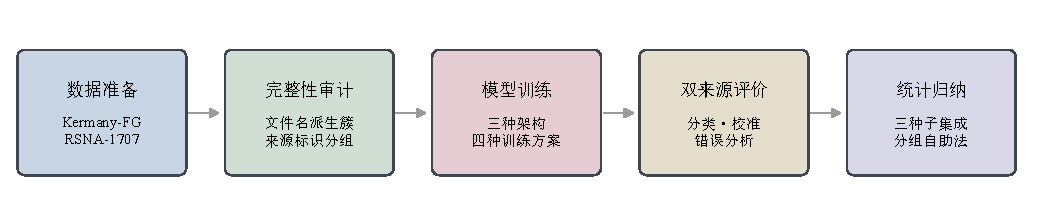
\includegraphics[width=0.80\textwidth]{figures/fig01_research_workflow.pdf}
  \caption{总体技术路线。Kermany 使用文件名派生簇进行保守分组，不能等同于经元数据确认的患者级隔离；RSNA 使用 patientId 分组。}
  \label{fig:research_workflow}
\end{figure}

\section{国内外研究现状}

\subsection{胸片深度学习分类研究}

胸片图像的自动分类是医学影像深度学习领域一个很受关注的方向。2017 年，Rajpurkar 等人发布的 CheXNet 是这个领域的一项重要工作，作者基于 DenseNet121 架构，在包含 112,120 张正面胸片的 NIH ChestX-ray14 数据集上训练了一个 14 类病理检测模型。该模型在肺炎检测任务上的 ROC-AUC 达到 0.9687，经 Board-certified 放射科医生的盲法对比评估，CheXNet 的肺炎检测灵敏度和特异度都不逊于四位放射科医生的平均水平\cite{rajpurkar2017}。这项研究引起了学术界对深度学习胸片分析的广泛关注，NIH ChestX-ray14 也成为后续研究中使用最广泛的公开基准数据集之一。

2018 年，Kermany 等人在《Cell》上发表了题为"Identifying Medical Diagnoses and Treatable Diseases by Image-Based Deep Learning"的研究\cite{kermany2018}。该研究使用基于 ImageNet 预训练的 Inception-v3 模型对 OCT 图像和儿科胸片进行分类，并公开了 Chest X-Ray Images (Pneumonia) 数据集，也就是本课程设计使用的 Kermany 数据集。该数据集来自广州妇女儿童医疗中心，共 5,856 张经过筛选的胸片图像，目录标签为 NORMAL（正常）和 PNEUMONIA（肺炎）；部分肺炎图像的文件名中还带有 bacteria（细菌性）或 virus（病毒性）标记。本课程设计使用的是 NORMAL 与 PNEUMONIA 二分类，病原体标记只用于理解文件命名和执行保守分组，不作为独立预测类别。

2018 年同期，北美放射学会（Radiological Society of North America, RSNA）在 Kaggle 上举办了 RSNA Pneumonia Detection Challenge 竞赛\cite{rsna2018}。与大多数分类任务不同，这个竞赛的任务是目标检测，在胸片图像中定位肺部阴影（opacity）的边界框，而不是简单地判断整张图像有没有肺炎。竞赛提供了超过 26,000 张来自临床 PACS 系统的 DICOM 格式正面胸片，标签由多位放射科医生标注。这个竞赛进一步丰富了公开可用的胸片数据资源，也推动了检测和分割模型在医学影像中的应用。

\subsection{卷积神经网络架构的演进}

我们选用的深度学习模型覆盖了 CNN 架构演进中的三个代表性节点。

DenseNet（Densely Connected Convolutional Network）由 Huang 等人于 2017 年在 CVPR 上提出\cite{huang2017}，其核心创新是密集连接（Dense Connectivity）机制：网络中每一层的输入由前面所有层的特征图在通道维度上拼接而成，即 $\mathbf{x}_l = H_l([\mathbf{x}_0, \mathbf{x}_1, \ldots, \mathbf{x}_{l-1}])$。这一设计带来了三个好处：（1）特征重用，浅层特征可以直接被深层使用，无需逐层传递而导致信息衰减；（2）梯度流动，损失函数的梯度可以通过密集连接直接回传到浅层，有效缓解深层网络的梯度消失问题；（3）参数效率，通过控制增长率（Growth Rate）$k=32$ 来限制每层新增特征通道数，DenseNet121 仅需约 800 万个参数即可取得与参数量大得多的 ResNet 相当的性能。在医学影像分析领域，DenseNet121 凭借其参数效率高、在小数据集上不易过拟合的优势，成为最广泛使用的骨干网络之一。

ConvNeXt 由 Liu 等人于 2022 年在 CVPR 上提出\cite{liu2022}，它的设计思路是从 ResNet-50 出发，逐一审视 Vision Transformer 的设计元素能否用来"现代化"标准 CNN，具体做了以下修改：（1）使用 7×7 大核深度可分离卷积替代 3×3 小核标准卷积，扩大感受野；（2）将激活函数从 ReLU 替换为 GELU；（3）将归一化层从 BatchNorm 替换为 LayerNorm；（4）采用倒置瓶颈（Inverted Bottleneck）结构，即中间层的通道数大于输入和输出通道数；（5）减少归一化和激活函数的使用频率。经过这一系列改造，ConvNeXt 在 ImageNet-1K 上的 Top-1 准确率超越了同等计算量的 Swin Transformer，说明标准 CNN 吸收 Transformer 的设计理念后仍然很有竞争力。我们选用 ConvNeXt-Tiny（约 2,800 万参数）作为现代 CNN 的代表，看看它在医学影像任务上的表现。

\subsection{Vision Transformer 及其在医学影像中的探索}

Vision Transformer（ViT）由 Dosovitskiy 等人于 2021 年在 ICLR 上发表\cite{dosovitskiy2021}，将 Transformer 架构从自然语言处理带入了计算机视觉领域。ViT 的核心思想是将二维图像分割为固定大小的 Patch（如 16×16 像素块），将每个 Patch 线性投影为固定维度的向量（类似于 NLP 中的词嵌入），再加上位置编码后作为标准 Transformer 编码器的输入序列。Transformer 编码器由多头自注意力（Multi-Head Self-Attention, MHSA）和多层感知机（MLP）交替堆叠而成，通过自注意力机制建模序列中任意两个位置之间的全局依赖关系：

\begin{equation}
\text{Attention}(\mathbf{Q}, \mathbf{K}, \mathbf{V}) = \text{softmax}\left(\frac{\mathbf{Q}\mathbf{K}^T}{\sqrt{d_k}}\right)\mathbf{V}
\end{equation}

其中 $\mathbf{Q}$、$\mathbf{K}$、$\mathbf{V}$ 分别为查询（Query）、键（Key）和值（Value）矩阵，$d_k$ 为键向量的维度。与 CNN 依赖局部感受野的层级式特征提取方式不同，ViT 从第一层开始就具备全局感受野，能够直接建模图像中远距离像素之间的依赖关系。

在医学影像分析领域，ViT 的应用仍处于探索阶段。一些研究表明，当训练数据充足时，ViT 在医学影像分类任务上可以达到甚至超过 CNN 的性能；但在数据量有限的情况下，ViT 缺少 CNN 的平移等变性和局部性归纳偏置（Inductive Bias），可能出现过拟合或收敛不稳定。本研究选用 ViT-B/16（ViT-Base, Patch 16×16，约 8,600 万参数）作为基于自注意力的架构代表，用于考察其跨来源表现。

\subsection{域偏移与跨来源评估}

域偏移（Domain Shift）是指训练数据（源域）和测试/部署数据（目标域）来自不同概率分布的现象。在经典统计学习理论中，大多数机器学习算法，包括经验风险最小化（ERM），都假设训练数据和测试数据独立同分布（i.i.d.），即 $\{(x_i, y_i)\}_{i=1}^n \overset{i.i.d.}{\sim} P(X,Y)$。当这一假设被违反时，在源域上最小化经验风险所学到的决策函数 $f$ 在目标域上的期望风险可能远高于在源域上的表现\cite{gulrajani2021}。

Gulrajani 和 Lopez-Paz（2021）在《In Search of Lost Domain Generalization》中对域泛化（Domain Generalization, DG）领域的多种算法进行了大规模实验评估\cite{gulrajani2021}。他们的研究发现：在严格的实验条件下（包括合理的超参数调优和充分的模型容量），经验风险最小化（ERM）基线在绝大多数 DG 基准测试中的表现与专门设计的 DG 算法（如 IRM、CORAL、DANN 等）没有显著差异。这个发现对域泛化研究的方法论提出了挑战，也说明在跨域场景下，严谨的实验设计（多来源测试、固定随机种子、合理的评价指标）可能比算法创新本身更重要。

在医学影像领域，域偏移问题尤其值得关注，因为它直接关系临床后果。医学影像的域偏移可能来源于以下多个层面：（1）设备层面，不同厂商的 X 光机、不同的成像参数（kVp、mAs）、不同的图像后处理算法导致图像的对比度、噪声水平和灰度分布存在差异；（2）人群层面，不同医疗机构的患者人口统计学构成（年龄、性别、基础疾病谱）不同，导致疾病表现的条件分布 $P(Y|X)$ 或 $P(X|Y)$ 存在差异；（3）标注层面，不同数据集采用的标签定义和标注流程不同（如临床诊断 vs 放射学征象描述 vs 竞赛任务目标），导致"同一类别标签"在语义上并不严格等价；（4）采集协议层面，后前位（PA）vs 前后位（AP）、立位 vs 卧位、是否吸气末屏气等因素均会影响胸片的外观和病变可见性。

Zech 等人（2018）比较了来自三个医疗系统的胸片模型，发现院内测试与跨医疗系统测试之间存在明显的性能差异，且图像中包含较强的来源信息\cite{zech2018}。这说明医院来源及其相关因素可能成为模型可以利用的混杂线索。DeGrave 等人（2021）在 COVID-19 胸片检测中也发现，多种模型依赖数据来源相关的捷径，而非稳定的病理信号\cite{degrave2021}。

这些研究表明，仅靠单一来源保留测试集上的性能指标来评价一个医学影像分类模型是远远不够的。跨来源评估，将模型在未参与训练的数据来源上进行测试，应当成为医学影像深度学习研究的常规做法。但目前大多数公开的胸片分类研究仍然主要依赖单一数据集的 train/test 划分报告性能，缺少对跨来源泛化能力的评估。

\section{存在的主要问题}

综合上述研究现状，本课题关注的核心问题可以归纳为以下四个方面。

\textbf{第一，单一数据集评估的局限性经常被低估。} 目前主流的胸片分类研究做法是：选择一个公开数据集（如 Kermany 或 NIH ChestX-ray14），按数据集自带的 train/val/test 划分或随机划分进行训练和评价，然后把测试集上的性能指标当作模型的"泛化能力"来报告。这个做法隐含了一个假设，测试集和训练集来自相同的数据分布，但在临床真实场景中，这个假设几乎从不成立。一个在广州儿童医院数据上训练的肺炎分类模型，部署到美国成人急诊数据上时，性能还能不能保持？这个问题关乎模型能否安全使用，但在目前的文献中，对它的实验关注远远少于对新算法的关注。

\textbf{第二，不同数据集之间的标签语义差异容易被忽视。} 以本课程设计使用的两个数据集为例：Kermany 数据集的标签来自临床诊断，经过治疗的肺炎患者 vs 检查后排除了肺炎的个体，标签的语义是"患有/不患有肺炎（作为临床疾病）"。而 RSNA 竞赛的标签来自放射科医生对图像中是否存在肺部阴影（lung opacity）的标注\cite{rsna2018}，"Target=1"表示图像中含有和肺炎相关的阴影区域，语义是"含有/不含符合肺炎表现的影像学征象"。在医学上，"影像学有阴影"和"临床确诊肺炎"并不严格等价，某些非感染性疾病（如肺水肿、肺不张）也可以表现为肺部阴影，而某些早期肺炎可能在胸片上还看不到明显阴影。当两个数据集被统一映射为 NORMAL/PNEUMONIA 二分类时，这个语义差异就被掩盖了，跨数据集的性能比较也因此建立在有问题的前提之上。

\textbf{第三，医学影像研究必须谨慎处理相关样本跨划分的问题。} 同一受试者的多次检查如果同时进入了训练集和测试集，模型的性能可能会被高估。Kermany 数据集的公开元数据没有提供可以独立核验的患者标识符，因此无法确认原始 train/val/test 目录是否实现了严格的患者级隔离。我们根据文件名构造了保守簇，把同一簇的图像放在同一划分中，以减少相关样本跨划分的风险。需要说明的是，文件名派生簇只是一种风险控制手段，不能等同于经过了临床元数据确认的患者身份。

\textbf{第四，深度学习实验的可复现性面临多重挑战。} 可复现性不仅仅是公开代码的问题，还涉及随机种子、数据划分、预处理参数、超参数搜索空间、CUDA 算子确定性模式等大量隐性变量的控制。Pineau 等人（2021）在 NeurIPS 的可复现性挑战中发现，即便作者积极配合，仍有大量论文的结果无法被第三方独立复现。在医学影像领域，数据集下载权限的时效性、DICOM 格式的解析差异、不同来源数据下载不全等因素进一步增加了复现难度。因此，建立一套覆盖数据审计、实验管理、结果验收的完整可复现流程，既是本课程设计的工程需要，也是一个值得做的方法探索。

\section{选题意义及必要性}

本课题的选题意义可以从以下几个方面来说明。

\textbf{理论方面：对比不同架构在跨来源场景下的表现。} 目前域泛化文献中，针对不同骨干架构（经典 CNN vs 现代 CNN vs Transformer）在相同训练条件下跨域泛化性能的系统对比还不多。我们在统一的实验平台上对 DenseNet121、ConvNeXt-Tiny 和 ViT-B/16 进行对比，控制训练配置（学习率、批量大小、预训练权重来源）和随机种子一致，希望能比较干净地回答"换架构能不能缓解域偏移"这个问题。同时，四种训练方案（ERM、ERM-Reg、JT、JT-DBS）从单来源无约束训练到多来源均衡训练的逐步推进，也为理解训练数据构成对跨来源泛化的影响提供了一条消融分析的思路。

\textbf{实践方面：建立一套全流程可复现的实验流程。} 这次课程设计的工程产出不仅是实验结果，还包括从数据 SHA-256 哈希核验、文件名分组审计，到 101 步自动化流程编排、51 项 pytest 测试，再到基于分组自助法的统计推断和自动验收程序\footnote{项目名称 CXRShift，代码开源，遵循 MIT License。}。这套流程可以迁移到其他医学影像分类任务的跨来源评估中。

\textbf{临床方面：为安全部署前的多来源验证提供实验参考。} 在深度学习辅助诊断系统从实验室走向临床的过程中，监管机构和临床用户最关心的问题之一就是模型在新环境中的泛化能力。我们在 Kermany 和 RSNA 两个来源差异很大的数据集上获得的对比结果，源域 97\% 的平衡准确率迁移到目标域后降至 66\%，为所有希望在临床场景中部署胸片 AI 模型的研究者和开发者提供了一个具体的警示数字。

\textbf{课程学习方面：理解实验环节之间的联系。} 本次实践把数据准备、模型选择、训练、评估和错误分析放在同一研究问题下考察。由此可以看到，数据划分和评价协议等看似基础的选择，也会直接影响性能估计及其可信度。

\section{本文主要工作与章节安排}

本文围绕胸片肺炎二分类中的跨来源域偏移问题，完成了以下主要工作：

\begin{enumerate}[label=(\arabic*)]
  \item \textbf{多架构多方案的对比实验。} 基于 PyTorch 框架，实现了 DenseNet121、ConvNeXt-Tiny 和 Vision Transformer (ViT-B/16) 三种架构，以及经验风险最小化（ERM）、正则化增强训练（ERM-Reg）、联合训练（JT）和域均衡采样联合训练（JT-DBS）四种训练方案，在 42/43/44 三个随机种子下共执行 18 次训练。
  \item \textbf{双数据集多维度的评估。} 在 Kermany 儿科胸片数据集（5,856 张）和 RSNA 成人胸片子集（1,707 张）上，从分类性能、概率校准、错误模式、来源可分性和抽样不确定性五个角度进行了评估。
  \item \textbf{全流程可复现的工程实践。} 实现了从数据完整性审计、配置驱动训练、逐图预测输出、温度缩放校准到 5000 次分组自助法统计推断的自动化流程，并通过 51 项 pytest 测试和自动验收程序确保结果可复现。
\end{enumerate}

本文共分为五章，各章内容安排如下：

\textbf{第一章 课题概述}（即本章）：介绍胸片肺炎分类的研究背景，综述深度学习胸片分析和域偏移领域的研究现状，分析当前存在的主要问题，说明选题意义，并概述本文的主要工作和章节组织。

\textbf{第二章 算法分析}：从任务约束和数据条件导出实验设计，说明 DenseNet121、ConvNeXt-Tiny 和 ViT-B/16 的选型依据，并给出 ERM、ERM-Reg、JT、JT-DBS 四种训练方案及校准、来源可分性和统计推断方法。

\textbf{第三章 试验系统设计}：给出系统的总体分层架构设计，描述代码组织、核心类设计和设计模式应用（配置-代码分离、工厂模式、门面模式），规范系统的输入输出格式和数据流设计，并逐一说明数据准备、模型训练、模型评价、概率校准、三随机种子集成与自助法统计等核心模块的处理流程。

\textbf{第四章 软件实施与实验运行}：记录软件系统实施过程（开发环境、关键步骤、调试中遇到的问题与解决方案），报告数据集验证与审计的结果（目录结构验证、统计信息、完整性审计、自动化测试），并呈现和分析主要实验结果（跨来源性能对比、混合训练方案对比、概率校准效果、来源可分性诊断、错误模式分析和统计显著性检验）。

\textbf{第五章 结束语}：总结主要结论，交流通过课程设计对模式识别学科的认识与体会，说明每位组员的工作划分，并讨论未来的研究方向。\vspace{0.5cm}

\textbf{附录}：提供补充实验结果，包括各随机种子详细指标、温度缩放校准完整结果和来源特征均值完整对比。

% ======================== 第二章 算法分析 ========================
\chapter{算法分析}

本章从任务约束、数据条件和评价目标出发确定实验方案。模型部分解释三种骨干网络的差异及选型范围；训练部分给出四种方案的目标函数和实施条件；分析部分说明校准、来源可分性与分组自助法分别回答什么问题。

\section{需求分析}

\subsection{功能需求}

本系统的核心目标是构建一个可审计、可复现的胸片肺炎二分类深度学习实验平台。从用户角色和实验流程两个角度看，系统的功能需求包括以下几个方面。

\textbf{二分类推理功能}：系统能接收单张胸片图像（JPEG 或 PNG 格式），输出预测类别（NORMAL / PNEUMONIA）及 Softmax 概率分数。推理功能支持本地 Web 界面（Flask + Gradio），允许用户上传图像、调整决策阈值并实时查看结果，同时以中文标签显示判断倾向。

\textbf{批量训练功能}：系统提供配置驱动的训练入口，支持通过 YAML 配置文件或命令行参数指定模型架构（DenseNet121 / ConvNeXt-Tiny / ViT-B/16）、训练策略（ERM / ERM-Reg / JT / JT-DBS）、超参数（学习率、批量大小、训练轮数、权重衰减等）和随机种子。训练过程自动记录每个 epoch 的训练损失与准确率、验证损失与准确率，并基于验证损失自动保存最佳检查点。

\textbf{模型评估功能}：系统在指定数据集划分上逐图推理，生成包含图像路径、真实标签、预测标签、NORMAL 概率和 PNEUMONIA 概率五列的预测 CSV 文件。基于逐图预测，自动计算混淆矩阵及准确率（Accuracy）、平衡准确率（Balanced Accuracy）、精确率（Precision）、召回率（Recall / 灵敏度）、特异度（Specificity）、F1 分数、ROC-AUC 和 AUPRC 共八项分类指标，并以 JSON 格式输出结构化评估报告。

\textbf{概率校准功能}：系统从验证集预测中学习温度缩放（Temperature Scaling）参数，将校准后的温度应用于测试集预测概率，计算并报告期望校准误差（ECE）、最大校准误差（MCE）、Brier 分数和负对数似然（NLL），生成校准前后的可靠性图（Reliability Diagram）。

\textbf{错误分析与可解释性功能}：系统按四桶策略（极端假阳性、极端假阴性、阈值附近假阳性、阈值附近假阴性）从预测结果中选取代表性错误样本，生成错误案例网格图和逐样本的 Grad-CAM 类激活热力图。

\textbf{可复现性验收功能}：系统提供全流程自动化编排入口，支持一次性执行从数据准备、训练、评价到分析的全部 101 步操作，自动检查数据身份（SHA-256 哈希核验）、实验矩阵完整性（必需实验的产物是否存在）和主要指标偏差（与发布值的相对误差是否小于 5\%），生成通过（VERIFIED）或失败的验收报告。

\subsection{数据需求}

本系统使用两个公开的胸部 X 光图像数据集，二者在来源机构、患者人群、标签语义和图像格式上存在明显差异，这恰好构成了跨来源压力测试的条件。

\textbf{Kermany 儿科胸片数据集}：原始数据来自广州妇女儿童医疗中心，由 Kermany 等人公开于 Mendeley Data（DOI: 10.17632/rscbjbr9sj.2），许可协议为 CC BY 4.0\cite{kermany2018}。该数据集包含 5,856 张经过筛选的后前位（PA）儿科胸片 JPEG 图像，分为 NORMAL（正常，1,583 张）和 PNEUMONIA（肺炎，4,273 张）两个类别，肺炎样本的文件名中还标注了 bacteria（细菌性）和 virus（病毒性）的病原体亚型。下载包自带 train（5,216 张）、val（16 张）和 test（624 张）三个目录划分。由于公开元数据中未包含可核验的患者标识符，本系统采用保守的文件名派生簇分组策略，将共享相同文件名前缀（如 \texttt{person100}）的不同子类型图像归为同一簇，按簇重新分配 train/val/test 划分，形成 Kermany-FG（File-Grouped）数据集，测试集包含 1,170 张图像共 624 个文件名簇。

\textbf{RSNA 成人胸片数据集}：来自 RSNA Pneumonia Detection Challenge\cite{rsna2018}（Kaggle, 2018），共包含 26,684 张 DICOM 格式的正面胸片，标签为目标肺部阴影（Lung Opacity）的存在与否。本系统从官方完整训练集中按冻结清单精确抽取 1,707 个 patientId 成员作为固定工作子集（RSNA-1707），按 patientId 分层随机划分为 train（70\%, 1,052 张）、val（10\%, 213 张）和 test（20\%, 442 张），随机种子为 42。DICOM 图像经最小--最大归一化后转为 8 位 PNG 格式，统一尺寸为 224×224 像素。

\textbf{数据完整性需求}：所有图像文件在进入训练管线前必须通过目录结构验证（train/val/test × NORMAL/PNEUMONIA 六目录完整且非空）、图像可读性验证（Pillow Image.verify()）和 SHA-256 哈希核验（与冻结清单逐项比对）。数据准备脚本默认拒绝覆盖已有输出，确保已审计数据的稳定性。

\subsection{性能需求}

\textbf{分类性能目标}：在源域（Kermany-FG 测试集）上，集成三种子的平衡准确率应不低于 95\%；在目标域（RSNA-1707 测试集）上，平衡准确率应不低于 60\%，后者明显低于前者，这正是域偏移的直接体现。

\textbf{计算效率需求}：单次 ERM 训练（DenseNet121，5 epochs，batch\_size=32，224×224 输入分辨率）在单块 NVIDIA GPU（≥8 GB 显存）上的耗时应在 30 分钟以内。全实验矩阵（18 次训练）可在单 GPU 上一昼夜内完成。

\textbf{可复现性需求}：所有训练使用固定的伪随机数种子（42 / 43 / 44），并启用 CUDA 确定性模式（\texttt{torch.backends.cudnn.deterministic = True}，\texttt{torch.backends.cudnn.benchmark = False}）。每次训练的完整配置（模型、超参数、数据划分、增强策略）随训练产物（JSON 报告 + PT 检查点）一同持久化。对任何第三方在相同软件和硬件环境下重建的结果，主要集成指标与发布值的相对偏差应小于 5\%。

\subsection{可复现性需求}

可复现性需求贯穿本系统设计的每一个环节，它不是独立的功能模块，而是对所有模块的共同约束：（1）\textbf{数据身份锁定}，Kermany 的 5,856 张图像和 RSNA 的 1,707 个 DICOM 成员必须全部通过冻结的 SHA-256 清单核验，任何文件缺失或哈希不匹配均应导致流程终止；（2）\textbf{实验矩阵可追溯}，每次训练的 YAML 配置、命令行参数、随机种子和产物路径遵循统一的命名协议（\texttt{CXRShift\_\_\{model\}\_\_\{recipe\}\_\_s\{seed\}}），确保任意一次训练的配置和产物的对应关系仅通过文件名即可唯一确定；（3）\textbf{自动化验收}，验收脚本（\texttt{verify\_reproduction.py}）自动检查必需实验结果的存在性、数据身份的完整性和主要指标的一致性，任何人可以一条命令复现验收判断。

\section{研究方案设计}

\subsection{对比实验设计}

本课程设计的核心实验问题可以分解为两个：（1）在相同训练条件下，不同深度学习架构（经典 CNN vs 现代 CNN vs Transformer）的跨来源泛化性能有没有系统性差异？（2）固定架构（DenseNet121）下，不同训练策略（单来源 vs 联合训练 vs 域均衡联合训练）能不能有效缓解跨来源性能衰减？

为回答这两个问题，我们设计了两个维度的受控对比。

\textbf{架构对比维度}：选定 DenseNet121（约 8M 参数）、ConvNeXt-Tiny（约 28M 参数）和 ViT-B/16（约 86M 参数）三种架构，分别在 Kermany-FG 训练集上以 ERM 策略训练，在 Kermany-FG 和 RSNA-1707 两个测试集上分别评估，观察架构选择对跨来源泛化的影响。

\textbf{训练策略对比维度}：固定 DenseNet121 架构，对比四种训练方案的跨来源性能：（1）ERM，仅在 Kermany-FG 上训练，作为单来源基线；（2）ERM-Reg，在 ERM 基础上增加颜色扰动和 0.1 标签平滑；（3）JT，将 Kermany 和 RSNA 训练数据合并后联合训练；（4）JT-DBS，在 JT 的基础上引入按图像来源（Kermany / RSNA）均衡的加权采样。（1）和（2）的对比可以看到训练正则化对泛化的影响，（1）、（3）和（4）的对比可以看到训练数据来源构成和采样策略对泛化的影响。

为减少单次训练随机性的干扰，每种配置使用随机种子 42、43 和 44 分别训练三次，测试时将三个种子的 Softmax 阳性概率取算术平均，在集成概率上计算所有指标。这样做的考虑是：单个随机种子反映了优化过程中对局部极小值的随机选择，三个种子取平均可以部分平滑这种方差，更稳健地估计给定配置下的期望性能。

\subsection{评价指标体系}

我们的评价指标覆盖分类准确性、概率质量和统计可靠性三个方面。

\textbf{分类准确性指标}。设 TP、TN、FP、FN 分别表示真正例、真负例、假正例和假负例的计数，定义以下指标：

\begin{equation}
\text{Accuracy} = \frac{TP + TN}{TP + TN + FP + FN}
\end{equation}

\begin{equation}
\text{Balanced Accuracy} = \frac{1}{2}\left(\frac{TP}{TP + FN} + \frac{TN}{TN + FP}\right)
\end{equation}

\begin{equation}
\text{Precision} = \frac{TP}{TP + FP}, \quad
\text{Recall (Sensitivity)} = \frac{TP}{TP + FN}
\end{equation}

\begin{equation}
\text{Specificity} = \frac{TN}{TN + FP}, \quad
F_1 = 2\cdot\frac{\text{Precision} \cdot \text{Recall}}{\text{Precision} + \text{Recall}}
\end{equation}

平衡准确率是本研究的主要指标，因为它分别计算两类召回率后取平均，可减轻类别比例对总体准确率的影响（Kermany 测试集中 PNEUMONIA 约占 62.5\%）。ROC-AUC 和 AUPRC 用于补充描述与固定阈值无关的排序性能。

\textbf{概率校准指标}。预测概率的可靠性通过以下指标评估：

\begin{equation}
\text{Brier Score} = \frac{1}{N}\sum_{i=1}^{N}(p_i - y_i)^2
\end{equation}

\begin{equation}
\text{ECE} = \sum_{m=1}^{M}\frac{|B_m|}{N}\left|\text{acc}(B_m) - \text{conf}(B_m)\right|
\end{equation}

其中 $M=10$ 为置信度桶数，$B_m$ 为第 $m$ 个等宽置信度区间内的样本集合，$\text{acc}(B_m)$ 和 $\text{conf}(B_m)$ 分别为该桶内的实际准确率和平均预测置信度。ECE 越小，模型的概率输出越接近真实似然。最大校准误差 MCE 取所有桶中差距的最大值。

\textbf{域偏移量化指标}。以来源可分性 AUROC 作为域偏移程度的间接度量：在 Kermany 和 RSNA 图像的均匀子样本上提取 11 个手工设计的像素级统计特征（均值、标准差、p10、中位数、p90、边界均值与标准差、中心均值与标准差、宽高比、熵），训练一个简单的逻辑回归分类器，以 AUROC 衡量仅凭低层图像统计特征区分来源的难易程度。在标签匹配条件（控制正负类别分布相等）下的 AUROC 是我们关注的域偏移主诊断量。

\textbf{统计推断方法}。我们的核心结论不依赖于单次评估的点估计。对 Kermany 测试集使用 624 个文件名簇作为分组单位，对 RSNA 测试集使用 442 个 patientId 作为分组单位，进行 5000 次非参数百分位数分组自助法（Grouped Bootstrap）。每次重采样中保持分组结构不变（同一簇/patientId 的图像同时出现或同时不出现），在集成概率上重新计算全部指标，以 2.5th 和 97.5th 百分位数作为 95\% 置信区间。候选方案与基线的成对比较在同一重采样中计算差值，从而获得配对差值分布而非独立分布的重叠检验。

\subsection{实验矩阵}

综合以上设计，我们共执行 \textbf{18 次正式训练}，实验矩阵见表~\ref{tab:exp_matrix}。

\begin{table}[htbp]
\centering
\caption{完整实验矩阵（共 18 次训练）}
\label{tab:exp_matrix}
\renewcommand{\arraystretch}{1.3}
\begin{adjustbox}{max width=\textwidth,center}
\begin{tabular}{ccllc}
\toprule
\textbf{实验族} & \textbf{模型} & \textbf{训练数据} & \textbf{训练方案} & \textbf{随机种子} \\
\midrule
ERM & DenseNet121      & Kermany-FG & 加权交叉熵                  & 42, 43, 44 \\
ERM & ConvNeXt-Tiny    & Kermany-FG & 加权交叉熵                  & 42, 43, 44 \\
ERM & ViT-B/16         & Kermany-FG & 加权交叉熵                  & 42, 43, 44 \\
ERM-Reg & DenseNet121  & Kermany-FG & 加权交叉熵 + 颜色扰动 + LS   & 42, 43, 44 \\
JT   & DenseNet121     & Kermany + RSNA 混合 & 加权交叉熵            & 42, 43, 44 \\
JT-DBS & DenseNet121   & Kermany + RSNA 混合 & 加权交叉熵 + 域均衡采样 & 42, 43, 44 \\
\bottomrule
\end{tabular}
\end{adjustbox}
\end{table}

图~\ref{fig:reproducibility_chain} 概括了从数据身份锁定到机器验收的证据链。图中每一环节均对应仓库中可检查的产物，确保模型指标与其数据来源、预测文件和统计口径保持一致。

\begin{figure}[htbp]
  \centering
  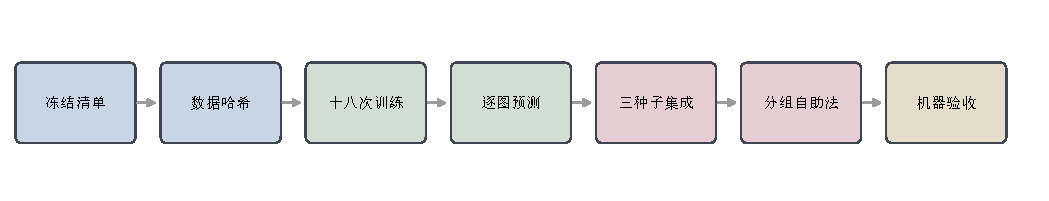
\includegraphics[width=0.80\textwidth]{figures/fig11_reproducibility_chain.pdf}
  \caption{实验结果的可复现证据链。18 次训练包括三种架构的 ERM 实验以及基于 DenseNet121 的 ERM-Reg、JT 和 JT-DBS 实验。}
  \label{fig:reproducibility_chain}
\end{figure}

每个训练完成的模型均在 Kermany-FG 测试集和 RSNA-1707 测试集上独立评估，共产生 36 组评估结果（18 次训练 × 2 个测试集）。所有评估均输出逐图预测 CSV 和结构化指标 JSON，确保后续的校准分析、错误分析和统计推断可以离线执行而无需重新加载模型。

\section{深度学习模型选择与分析}

本节对三种模型架构的算法原理进行分析。各架构的发展背景已在第一章中介绍，这里重点关注数学机制、结构配置以及在本任务中的具体适配方式。

\subsection{DenseNet121}

DenseNet121 是一个包含 121 层可训练权重的密集连接卷积网络，其核心结构由四个密集块（Dense Block）和三个过渡层（Transition Layer）交替组成\cite{huang2017}。

\textbf{密集连接的数学机制}。设第 $l$ 层的输入为前面所有层的特征图在通道维度上的拼接：

\begin{equation}
\mathbf{x}_l = H_l\left([\mathbf{x}_0, \mathbf{x}_1, \ldots, \mathbf{x}_{l-1}]\right)
\end{equation}

其中 $[\cdot]$ 表示通道维度的拼接操作，$H_l(\cdot)$ 是一个复合函数，在本实现中由 BatchNorm $\to$ ReLU $\to$ 3×3 卷积依次组成（即 pre-activation 设计）。令 $k_0$ 为输入层的通道数，$k$ 为增长率（Growth Rate），则第 $l$ 层的输入通道数为 $k_0 + k \times (l-1)$。DenseNet121 使用 $k=32$，在四个密集块中分别包含 6、12、24 和 16 个 $H_l$ 单元。

\textbf{过渡层的通道压缩}。密集块之间通过过渡层进行下采样和通道压缩。过渡层由 1×1 卷积和 2×2 平均池化组成，其中 1×1 卷积将输入通道数压缩为 $\lfloor\theta m\rfloor$，$m$ 为输入通道数，压缩因子 $\theta=0.5$。这一设计控制了随着网络加深通道数的指数增长趋势。

\textbf{分类头的替换}。原始 DenseNet121 的分类器为一个输出 1000 维的全连接层（对应 ImageNet-1K 类别）。本系统将其替换为一个随机初始化的 2 输出全连接层（对应 NORMAL 和 PNEUMONIA），使用 Kaiming 均匀初始化。仅当指定 \texttt{freeze\_mode=classifier} 时，除分类头以外的所有层参数被冻结。

\textbf{选型考量}。DenseNet121 相对于 ResNet-50 的优势在于参数效率高（约 8M vs 约 25M），在中小规模医学影像数据集上不容易过拟合。密集连接还提供了隐式的深度监督，浅层特征可以直接被深层损失函数约束，这对标注样本不多的医学影像任务比较有利。

\subsection{ConvNeXt-Tiny}

ConvNeXt-Tiny 是现代 CNN 架构的代表，其设计理念是"像 Transformer 一样构建 CNN"\cite{liu2022}。

\textbf{与标准 ResNet 的关键差异}。ConvNeXt-Tiny 对 ResNet 的每个结构组件进行了逐项审视和替换：（1）\textbf{阶段比例}：四个阶段的块数从 ResNet-50 的 (3, 4, 6, 3) 调整为 (3, 3, 9, 3)，更接近 Swin-T 的 (2, 2, 6, 2) 但保留更多浅层块以保证在 224×224 分辨率下的计算效率；（2）\textbf{Patchify 干}：使用 4×4、步长 4 的非重叠卷积替代 ResNet 的 7×7、步长 2 卷积作为输入端，匹配 ViT 的 Patch 划分策略；（3）\textbf{深度可分离卷积}：将 3×3 标准卷积替换为 7×7 深度可分离卷积（分组数等于输入通道数），在不同空间位置共享但通道间独立的卷积核，在增大感受野的同时控制参数量；（4）\textbf{倒置瓶颈}：将通道维度先扩展 4 倍（1×1 卷积）、再深度可分离卷积、再压缩回原维度，与 Transformer 的 MLP 块先扩张后收缩的结构一致；（5）\textbf{LayerNorm 替代 BatchNorm}：沿通道维度而非批次维度进行归一化，消除了 BatchNorm 在小批量下的统计不稳定性。

\textbf{各阶段通道数}：ConvNeXt-Tiny 四个阶段的输出通道数分别为 96、192、384、768，总参数量约 28M。

\textbf{选型考量}。ConvNeXt-Tiny 代表了一种思路，不引入自注意力机制，但通过结构现代化在 ImageNet 上达到与 Swin Transformer 相当的性能。在本课程设计中，它要回答的问题是："现代化 CNN 在跨来源医学影像任务上，会不会比经典 CNN 表现更好？"

\subsection{Vision Transformer (ViT-B/16)}

ViT-B/16 是 Vision Transformer 家族中最广泛使用的基准模型之一\cite{dosovitskiy2021}。

\textbf{Patch 嵌入}。输入图像 $\mathbf{x} \in \mathbb{R}^{H \times W \times C}$ 被划分为 $N = HW/P^2$ 个不重叠的 $P \times P$ 像素块，每个块通过可训练的线性投影矩阵 $\mathbf{E} \in \mathbb{R}^{(P^2 \cdot C) \times D}$ 映射为 $D$ 维嵌入向量。ViT-B/16 使用 $P=16$，$D=768$，对于 224×224 的输入图像，产生 $N=196$ 个 Patch 嵌入。

\textbf{可学习位置编码与分类 Token}。在 Patch 嵌入序列前添加一个可学习的 [CLS] Token $\mathbf{x}_{\text{class}} \in \mathbb{R}^D$，并加上可学习的一维位置编码 $\mathbf{E}_{\text{pos}} \in \mathbb{R}^{(N+1) \times D}$，形成 Transformer 编码器的完整输入序列：

\begin{equation}
\mathbf{z}_0 = [\mathbf{x}_{\text{class}}; \mathbf{x}_p^1\mathbf{E}; \mathbf{x}_p^2\mathbf{E}; \ldots; \mathbf{x}_p^N\mathbf{E}] + \mathbf{E}_{\text{pos}}
\end{equation}

\textbf{Transformer 编码器层}。每层编码器由多头自注意力（MHSA）和多层感知机（MLP）两个子层组成，每个子层前后均应用 LayerNorm 和残差连接：

\begin{equation}
\mathbf{z}'_{\ell} = \text{MHSA}\left(\text{LN}\left(\mathbf{z}_{\ell-1}\right)\right) + \mathbf{z}_{\ell-1}
\end{equation}

\begin{equation}
\mathbf{z}_{\ell} = \text{MLP}\left(\text{LN}\left(\mathbf{z}'_{\ell}\right)\right) + \mathbf{z}'_{\ell}
\end{equation}

MHSA 将 $D$ 维嵌入分给 $h$ 个注意力头（$h=12$，每头 64 维），在每个头上独立执行缩放点积注意力。MLP 由一个隐藏层（$4D=3072$ 维的 GELU 激活）和一个输出投影组成。ViT-B 共堆叠 $L=12$ 层编码器。最终取 [CLS] Token 的输出作为图像的全局表示，送入 2 输出的分类头。

\textbf{选型考量}。ViT-B/16 的参数量（约 86M）远大于 DenseNet121 和 ConvNeXt-Tiny，而且缺乏 CNN 的平移等变性归纳偏置，理论上来讲在小数据集上更容易过拟合。不过 ImageNet-21K 预训练提供了较强的视觉先验，有可能弥补这个劣势。

\subsection{ImageNet 预训练与迁移学习}

三种架构的训练均采用"ImageNet 预训练 + 下游微调"的迁移学习方法。DenseNet121 和 ConvNeXt-Tiny 使用 ImageNet-1K 预训练权重（torchvision 官方权重），ViT-B/16 使用 ImageNet-1K 的 ViT\_B\_16\_Weights。对于 DenseNet121 和 ConvNeXt-Tiny，由于分类头维度不同（ImageNet 1000 类 → 本任务 2 类），预训练的分类器权重被丢弃，替换为随机初始化的全连接层；对于 ViT-B/16，预训练的 heads.head 层被替换。所有其他层的预训练权重被保留，并在微调阶段参与梯度更新。

在具体实现中，模型创建通过工厂函数 \texttt{create\_classifier\_model()} 完成。该函数接收模型名称字符串（如 \texttt{"torchvision:densenet121"}）、类别数和预训练标志，内部根据名称分发到对应的 torchvision 模型构造函数。对于 DenseNet121，当 \texttt{pretrained=True} 时，函数加载 \texttt{DenseNet121\_Weights.IMAGENET1K\_V1} 权重，然后获取 \texttt{model.classifier.in\_features}（1024 维），将其替换为 \texttt{nn.Linear(1024, 2)}。ConvNeXt-Tiny 的替换方式类似，但其分类器位于 \texttt{model.classifier[-1]}（一个 Sequential 的最后一个 Linear 层），输入特征为 768 维。ViT-B/16 的分类头位于 \texttt{model.heads.head}，输入特征为 768 维。所有替换后的全连接层使用 Kaiming 均匀初始化。

\textbf{工厂函数的扩展性设计}。工厂函数不仅支持三种 torchvision 内置模型，还通过 \texttt{timm.create\_model()} 预留了使用 timm（PyTorch Image Models）库中数百种预训练模型的扩展能力。调用方只需传递一个 timm 模型名称（如 \texttt{"tf\_efficientnetv2\_s.in1k"}），工厂函数就会委托给 timm 进行模型创建、权重加载和分类头配置。这一设计使得在后续工作中尝试更多模型架构（如 EfficientNetV2、ConvNeXtV2、SwinV2 等）时，不需要修改训练脚本或评价脚本中的任何代码，只需在 YAML 配置文件中更改 \texttt{model} 字段，并确保 timm 库已安装。当前项目中虽然没有在正式实验中使用 timm 模型，但工厂函数的这一扩展能力已在单元测试中得到验证（\texttt{test\_inference.py} 中的 \texttt{test\_create\_classifier\_model\_timm} 测试创建了一个轻量级 timm 模型并验证了其输出维度）。

\textbf{预训练权重版本的一致性保障}。迁移学习中一个容易被忽视但可能导致不可复现结果的细节是预训练权重的版本管理。torchvision 的预训练权重会随着库版本的更新而变化，例如 \texttt{DenseNet121\_Weights.IMAGENET1K\_V1} 和 \texttt{IMAGENET1K\_V2} 是在不同训练配置（epoch 数、数据增强、优化器设置）下产生的权重，两者在同一任务上的微调结果可能存在差异。本系统通过在 YAML 配置文件中显式指定权重版本（在代码中硬编码 V1 变体），并在 \texttt{requirements.txt} 中固定 torchvision 版本，确保所有训练和复现均使用相同的预训练权重。验收脚本的"主要指标偏差 < 5\%"容限部分也考虑到了未来 torchvision 版本更新可能带来的权重变化，如果官方改变了默认的预训练权重，验收程序会检测到指标偏差并标记为失败，提示复现者检查环境配置。

\subsection{配置驱动的训练管理}

本系统的训练配置采用 YAML 文件与命令行参数双层覆盖机制。每个实验族对应一个 YAML 配置文件（存放于 \texttt{configs/} 目录），共包含四个 YAML 文件：

\begin{itemize}
  \item \texttt{DenseNet121\_\_ERM.yaml}：DenseNet121 的 ERM 基线训练配置；
  \item \texttt{ConvNeXt-Tiny\_\_ERM.yaml}：ConvNeXt-Tiny 的 ERM 训练配置；
  \item \texttt{ViT-B16\_\_ERM.yaml}：ViT-B/16 的 ERM 训练配置；
  \item \texttt{DenseNet121\_\_ERM-Reg.yaml}：DenseNet121 的正则化增强训练配置。
\end{itemize}

每个 YAML 配置文件采用四段结构。\texttt{project} 段定义任务名称和类别列表（\texttt{classes: ["NORMAL", "PNEUMONIA"]}）；\texttt{paths} 段指定数据、结果和检查点目录；\texttt{data} 段控制图像尺寸（224×224）、归一化方式（ImageNet 均值/标准差）和数据增强参数；\texttt{training} 段包含模型名称、预训练标志、训练轮数（DenseNet121 和 ConvNeXt-Tiny 为 5 epochs，ViT-B/16 为 4 epochs）、批量大小（32，ViT-B/16 为 16）、优化器参数和学习率调度器类型。

配置的加载遵循三级优先级：代码内置默认值 \texttt{DEFAULT\_CONFIG} → YAML 文件覆盖 → CLI 参数最终覆盖。合并操作由 \texttt{deep\_merge()} 函数递归执行，确保嵌套字典中的键被正确覆盖而非整段替换。合并后的配置被封装为不可变的 \texttt{TrainSettings} 数据类（\texttt{@dataclass(frozen=True)}），训练过程中任何对配置字段的意外修改都会触发运行时错误。

JT 和 JT-DBS 实验方案没有独立的 YAML 文件，而是通过 CLI 参数在 ERM 配置基础上动态调整。具体来说，JT 训练通过 \texttt{--data-root} 指向 Kermany 和 RSNA 的混合数据目录，JT-DBS 则额外添加 \texttt{--domain-balanced-prefixes kermany rsna} 参数来启用域均衡采样。这种设计使得新增一个实验方案只需要组合已有的配置文件和命令行参数，不需要修改任何 Python 代码。

\section{训练策略与优化算法}

\subsection{经验风险最小化 (ERM)}

设训练集 $\mathcal{D} = \{(x_i, y_i)\}_{i=1}^{n}$，其中 $x_i \in \mathcal{X}$ 为胸片图像，$y_i \in \{0, 1\}$ 为二值标签（0 = NORMAL，1 = PNEUMONIA）。分类器 $f_\theta: \mathcal{X} \to \mathbb{R}^2$ 为由参数 $\theta$ 参数化的神经网络，输出二维 logits 向量。Softmax 函数将 logits 转换为概率向量：

\begin{equation}
\hat{p}_\theta(c \mid x) = \frac{\exp\left(f_\theta(x)_c\right)}{\sum_{j=1}^{2} \exp\left(f_\theta(x)_j\right)}, \quad c \in \{0, 1\}
\end{equation}

经验风险最小化（ERM）的训练目标为最小化训练集上的加权交叉熵损失：

\begin{equation}
\mathcal{L}_{\text{ERM}}(\theta) = -\frac{1}{n}\sum_{i=1}^{n}\left[w_{y_i} \cdot \log \hat{p}_\theta(y_i \mid x_i)\right]
\end{equation}

其中类别权重 $w_c = n / (2 \cdot n_c)$，$n_c$ 为类别 $c$ 的训练样本数。加权机制确保模型不会偏向样本数更多的类别，在 Kermany 训练集中，PNEUMONIA 样本约为 NORMAL 的 2.7 倍，若不加权，模型可能学到倾向于预测 PNEUMONIA 的捷径。

\textbf{类别权重的具体计算}。以 Kermany-FG 训练集为例：NORMAL 类别的训练样本数 $n_{\text{NORMAL}} \approx 1113$，PNEUMONIA 类别的训练样本数 $n_{\text{PNEUMONIA}} \approx 2994$。总样本数 $n = n_{\text{NORMAL}} + n_{\text{PNEUMONIA}} \approx 4107$。根据加权公式：

\begin{equation}
w_{\text{NORMAL}} = \frac{4107}{2 \times 1113} \approx 1.845, \quad
w_{\text{PNEUMONIA}} = \frac{4107}{2 \times 2994} \approx 0.686
\end{equation}

按该公式计算，NORMAL 和 PNEUMONIA 的权重约为 1.845 和 0.686。少数类样本在损失中获得较大权重，多数类样本获得较小权重，使两类样本对总损失的期望贡献接近。这里比较的是按类别样本数加权后的总贡献，不能用两个权重的乘积判断是否平衡。

在 JT 和 JT-DBS 方案中，类别权重基于联合训练集（Kermany + RSNA）的全局类别频率重新计算。由于 RSNA-1707 的训练集类别接近平衡（NORMAL 560 张，PNEUMONIA 492 张），加入 RSNA 数据后联合训练集的 NORMAL 总数约为 1,673（1,113 + 560），PNEUMONIA 总数约为 3,486（2,994 + 492），总样本数约为 5,159，全局不平衡比降至约 1:2.08。因此 JT 方案中的类别权重要比纯 ERM 方案更均衡（$w_{\text{NORMAL}} \approx 1.542$，$w_{\text{PNEUMONIA}} \approx 0.740$），这在一定程度上减弱了模型对 PNEUMONIA 类别的偏向，可能与 JT 在 RSNA 上显著提高的特异度（0.8093 vs ERM 的 0.3535）有部分关联。

\textbf{ERM 在跨来源场景下的局限}。ERM 的统计保证建立在训练集和测试集同分布的假设之上：当 $P_{\text{train}}(X,Y) = P_{\text{test}}(X,Y)$ 时，$\mathcal{L}_{\text{ERM}}$ 的最小化等价于期望风险的最小化。但在跨来源场景中，$P_{\text{Kermany}}(X,Y) \neq P_{\text{RSNA}}(X,Y)$，此时 ERM 学到的决策函数在 RSNA 上的期望风险没有理论上界保证\cite{gulrajani2021}。

\subsection{正则化增强训练 (ERM-Reg)}

ERM-Reg 在 ERM 的基础上加入两个正则化组件：数据增强和标签平滑。

\textbf{数据增强}。训练时对每个批次的图像随机应用以下变换：（1）随机水平翻转，概率 $p=0.5$；（2）随机旋转，角度在 $[-7^\circ, 7^\circ]$ 范围内均匀采样；（3）颜色扰动，对亮度（±0.1）、对比度（±0.1）和饱和度（±0.05）进行小幅随机偏移。

训练增强包括随机水平翻转、小角度旋转和轻度颜色扰动。旋转范围限制为 ±7$^\circ$，颜色扰动仅用于 ERM-Reg。它们用于增加训练图像的外观变化，但本研究没有单独验证每种增强与设备参数或临床成像变化的对应关系，因此不对其医学真实性作进一步解释。

\textbf{ERM-Reg 与 ERM 增强策略的差异}。ERM 基线方案也使用了水平翻转和随机旋转作为基本增强，但 ERM-Reg 额外引入了颜色扰动和标签平滑。这一差异构成了 ERM vs ERM-Reg 消融对比的核心：两个方案在其他条件完全相同的情况下，后者的额外正则化能否带来可测的跨来源性能改善。实验结果（第四章）表明，在 RSNA 上 ERM-Reg 的平衡准确率（0.7233）显著高于 ERM（0.6591），提升幅度约为 6.4 个百分点，说明在单来源训练范式下，通过增强让模型接触更丰富的外观变异，确实有助于缓解跨来源的性能衰减，但改善仍然有限，远不及直接引入目标域数据的联合训练方案（0.7813）。

\textbf{ERM-Reg 的增强实现细节}。在代码层面，ERM-Reg 的数据增强流水线通过 torchvision 的 \texttt{transforms.Compose} 构建。训练变换包括：\texttt{Resize((224, 224))} → \texttt{RandomHorizontalFlip(p=0.5)} → \texttt{RandomRotation(degrees=7)} → \texttt{ColorJitter(brightness=0.1, contrast=0.1, saturation=0.05)} → \texttt{ToTensor()} → \texttt{Normalize(mean=[0.485, 0.456, 0.406], std=[0.229, 0.224, 0.225])}。评估变换仅保留 Resize、ToTensor 和 Normalize，不应用任何随机增强。ERM 基线的训练变换则省略 ColorJitter 步骤，其余完全相同。两种方案使用相同的 ImageNet 归一化参数，这是迁移学习的标准做法，预训练模型的权重是在 ImageNet 的统计分布上优化的，保持相同的归一化参数可以确保预训练特征的有效迁移。

\textbf{标签平滑}。不对硬标签 $y \in \{0, 1\}$ 直接计算损失，而是使用平滑后的软标签：

\begin{equation}
y^* = (1 - \alpha) \cdot y + \frac{\alpha}{K}
\end{equation}

其中 $\alpha=0.1$ 为平滑系数，$K=2$ 为类别数。标签平滑将正确类别的目标概率从 1.0 降至 0.95，将错误类别的目标概率从 0.0 升至 0.05。这防止了模型对训练标签的过度自信，在跨来源场景中可能有助于避免因过度依赖源域特有特征而导致的错误判断。

ERM-Reg 的损失函数与 ERM 相同（加权交叉熵），唯一区别是 $y_i$ 替换为 $y_i^*$。

\subsection{联合训练 (JT)}

联合训练将 Kermany 和 RSNA 两个来源的训练数据直接合并为一个联合训练集 $\mathcal{D}_{\text{JT}} = \mathcal{D}_{\text{Kermany}}^{\text{train}} \cup \mathcal{D}_{\text{RSNA}}^{\text{train}}$，使用与 ERM 相同的加权交叉熵损失进行训练。类别权重基于联合训练集中的全局类别频率计算。

JT 的想法很直接：如果模型在训练时能同时"看到"来自两个来源的图像，它就有机会学习跨来源共享的诊断特征，而不是只学习源域特有的分布特征。然而，JT 的一个潜在问题是来源不平衡，如果 Kermany 训练集（约 5,200 张）远大于 RSNA 子集（约 1,050 张），梯度更新将更多地由 Kermany 样本驱动，RSNA 样本的贡献被稀释，联合训练实际上几乎等同于单来源训练。

\textbf{JT 实验的具体配置}。JT 实验使用 \texttt{prepare\_mixed\_binary.py} 脚本构建混合数据目录。该脚本读取 Kermany-FG 和 RSNA-1707 的训练及验证划分，将两个来源的同名子目录（train/NORMAL、train/PNEUMONIA、val/NORMAL、val/PNEUMONIA）中的图像通过符号链接汇集到统一的输出目录中，保持 ImageFolder 格式不变。训练脚本通过 \texttt{--data-root} 指向混合目录，其余配置（模型、优化器、学习率调度）与 ERM 基线完全相同。JT 使用与 ERM 相同的加权交叉熵损失，类别权重 $w_c = n_{\text{total}} / (2 \cdot n_c)$ 基于联合训练集中两个来源的全局类别频率合并计算，这意味着如果两个来源的某一类样本合并后仍然占据多数，其权重会被压低；反之则被抬高。

JT 的训练过程中不引入任何来源标识信息，模型不知道每张图像来自 Kermany 还是 RSNA。这种"来源盲"设计是有意为之的：它测试的是"在有更多样化训练数据的情况下，模型是否能自发学到更通用的特征"，而不是"模型是否学会了区分数据来源"。JT 的局限性也正源于此，如果两个来源的条件分布 $P(Y|X)$ 本身不同，模型没有机制区分"这个样本是来自来源 A 的肺炎"和"这个样本是来自来源 B 的正常但外观类似来源 A 的肺炎"，两者在损失函数中被同等对待。

\subsection{域均衡采样联合训练 (JT-DBS)}

JT-DBS 在 JT 的基础上通过修改采样策略来解决来源不平衡问题。不使用标准的随机打乱（shuffle），而是使用 PyTorch 的 \texttt{WeightedRandomSampler}，为每个训练样本 $(x_i, y_i)$ 分配采样权重：

\begin{equation}
w_i = \frac{1}{N_{\text{source}(i)}}
\end{equation}

其中 $\text{source}(i) \in \{\text{kermany}, \text{rsna}\}$ 为样本 $i$ 的图像来源（通过文件名前缀确定），$N_{\text{source}(i)}$ 为该来源的训练样本总数。在这一权重方案下，每个训练批次中两个来源的图像具有相等的期望出现次数，无论二者的样本量差距多大。采样采用有放回方式（replacement=True），确保训练可以持续任意多个批次而不受小来源样本量的限制。

\textbf{JT-DBS 的局限}。域均衡采样通过改变训练数据的边缘分布 $P_{\text{train}}(\text{source})$ 来缓解来源不平衡，但它不改变条件分布 $P_{\text{train}}(X \mid \text{source})$ 或 $P_{\text{train}}(Y \mid \text{source})$。如果两个来源的任务条件分布本身就不一样（例如 RSNA 的"PNEUMONIA"标签在医学语义上和 Kermany 的"PNEUMONIA"不等价），仅仅均衡来源采样是无法从根本上解决标签语义差异问题的。

\subsection{优化算法}

所有训练统一使用 AdamW 优化器和余弦退火学习率调度。预训练骨干与随机初始化分类头的起点不同，本可为二者设置不同学习率；当前实验为控制变量，统一使用配置文件中的学习率。AdamW 根据参数的一阶矩和二阶矩调整更新幅度，并将权重衰减从梯度更新中解耦。这里的选择属于稳定、常用的训练基线，不意味着 AdamW 必然优于经过充分调参的 SGD。

标准 Adam 把 L2 正则项并入梯度，自适应缩放会同时作用于该项。AdamW 则直接从参数中减去 $\lambda\theta_t$，使权重衰减不再经过一阶矩和二阶矩缩放。本研究没有比较不同优化器，因此只说明实现依据，不据此声称 AdamW 改善了本任务的性能或泛化能力。

\textbf{AdamW 优化器}。AdamW 是 Adam 的解耦权重衰减变体，其参数更新规则为：

\begin{equation}
\theta_{t+1} = \theta_t - \eta\left(\frac{\hat{m}_t}{\sqrt{\hat{v}_t} + \epsilon} + \lambda\theta_t\right)
\end{equation}

其中 $\hat{m}_t$ 和 $\hat{v}_t$ 分别为一阶矩和二阶矩的偏差校正估计，$\eta$ 为学习率，$\lambda$ 为权重衰减系数。与标准 L2 正则化不同，AdamW 将权重衰减与自适应学习率解耦，在 $m_t$ 和 $v_t$ 的计算过程中不使用衰减后的 $\theta_t$。本系统使用默认的超参数 $\beta_1=0.9$，$\beta_2=0.999$，$\epsilon=10^{-8}$，学习率 $\eta=1\times10^{-4}$，权重衰减 $\lambda=1\times10^{-4}$。

\textbf{余弦退火学习率调度}。每个 epoch 的学习率按余弦曲线从初始值 $\eta_{\max}$ 衰减至 $\eta_{\min}$：

\begin{equation}
\eta_t = \eta_{\min} + \frac{1}{2}\left(\eta_{\max} - \eta_{\min}\right)\left(1 + \cos\left(\frac{t}{T_{\max}}\pi\right)\right)
\end{equation}

其中 $t$ 为当前 epoch（从 0 开始），$T_{\max} = 5$ 为总 epoch 数。余弦调度在训练初期保持较高的学习率以进行充分探索，在训练末期平缓衰减以在最小值附近精细收敛。

\textbf{混合精度训练}。当设备为 CUDA GPU 时，启用 PyTorch 的自动混合精度（Automatic Mixed Precision, AMP）。前向传播中，计算密集的卷积和矩阵乘法使用 FP16 半精度以提升吞吐量和节省显存；损失缩放（Loss Scaling）和 FP32 主权重副本确保数值稳定性。实际训练吞吐量约提升 1.5--2 倍，显存占用约降低 30\%。

\textbf{确定性配置}。为确保跨运行和跨机器的可复现性，训练环境进行如下确定性配置：（1）Python \texttt{random}、NumPy 和 PyTorch 的伪随机数生成器全部使用显式的种子初始化；（2）\texttt{torch.backends.cudnn.benchmark = False}，禁用 cuDNN 的自动算法搜索，强制每次运行使用相同的卷积实现；（3）\texttt{torch.backends.cudnn.deterministic = True}，仅选择 cuDNN 中具有确定性行为的算法。

\subsection{训练循环的详细实现}

训练循环（\texttt{run\_epoch} 函数）的设计是本系统训练模块的核心。该函数通过 \texttt{optimizer} 参数的有无自动区分训练和验证模式：

\begin{itemize}
  \item 当 \texttt{optimizer} 不为 None 时，函数以训练模式运行：设置 \texttt{model.train()}，对每个批次执行 \texttt{optimizer.zero\_grad(set\_to\_none=True)} → 前向传播 → 损失计算 → 反向传播 → 优化器步进。\texttt{set\_to\_none=True} 将梯度张量直接设为 None 而非填充零值，这在 PyTorch 中更高效且避免了不必要的内存分配。
  \item 当 \texttt{optimizer} 为 None 时，函数以验证模式运行：设置 \texttt{model.eval()}，在 \texttt{torch.no\_grad()} 上下文中仅执行前向传播和损失计算，不更新模型参数。\texttt{no\_grad()} 上下文禁用梯度计算图的构建，显著减少内存占用。
\end{itemize}

对于 AMP 混合精度训练，前向传播使用 \texttt{torch.cuda.amp.autocast} 上下文管理器。该上下文自动将符合条件的运算（卷积、矩阵乘法）降为 FP16 执行，同时保持对精度敏感的运算（Softmax、LayerNorm、损失计算）为 FP32。反向传播时，梯度缩放器 \texttt{GradScaler} 在 \texttt{scaler.scale(loss).backward()} 中将损失乘以一个动态缩放因子以防止 FP16 下小梯度变为零，然后在 \texttt{scaler.step(optimizer)} 中自动 unscale 梯度并执行参数更新，最后通过 \texttt{scaler.update()} 根据是否出现梯度溢出动态调整缩放因子。

每个 epoch 结束后，训练脚本记录当前 epoch 的训练损失/准确率和验证损失/准确率。如果当前 epoch 的验证损失优于历史最小值，则保存最佳检查点（\texttt{best.pt}）；同时始终保存最新检查点（\texttt{latest.pt}）。检查点文件以字典格式组织，包含以下键：\texttt{model\_state}（模型的 \texttt{state\_dict}）、\texttt{optimizer\_state}（优化器的 \texttt{state\_dict}）、\texttt{classes}（类别名称元组）、\texttt{settings}（训练配置字典，包括模型名称、图像尺寸、归一化方式、所有超参数）、\texttt{history}（每 epoch 的指标列表，每个条目包含 epoch 编号、训练损失/准确率和验证损失/准确率）。这种"检查点即文档"的设计确保任何一个检查点文件都是自包含的，从它出发可以完全重建模型、恢复训练或独立进行评价，无需查找原始 YAML 配置文件或命令行参数。

\section{概率校准与域偏移分析}

\subsection{概率校准：Temperature Scaling}

深度神经网络虽然分类准确率很高，但通过 Softmax 输出的概率通常过度自信（Overconfident），高置信度的预测并不对应同样高的实际正确率\cite{guo2017}。在医学影像场景中，校准不良的概率可能导致临床用户对模型的判断产生过度的信任。Temperature Scaling 是一种简单而有效的后处理校准方法：在验证集上学习单一温度参数 $T > 0$，将原始 logits 缩放后再输入 Softmax：

\begin{equation}
\hat{p}_i(T) = \text{softmax}\left(\frac{\mathbf{z}_i}{T}\right)
\end{equation}

$T=1$ 对应原始的未校准概率；$T>1$ 使概率分布更均匀（更保守）；$T<1$ 使概率分布更尖锐（更自信）。温度参数通过最小化验证集上的负对数似然（NLL）来确定：

\begin{equation}
T^* = \arg\min_{T}\ -\frac{1}{N}\sum_{i=1}^{N}\log \hat{p}_{i, y_i}(T)
\end{equation}

实验中在 $[0.5, 20.0]$ 区间内以 0.01 为步长进行网格搜索，选择使验证集 NLL 最小的 $T$。温度缩放的一个重要性质是它不改变模型排序：argmax 预测在任意 $T>0$ 下保持不变，只调整概率分布的尖锐程度。因此，在二分类阈值为 0.5 时，预测标签和混淆矩阵保持不变，概率数值及其可靠性指标则会发生变化。

\textbf{校准评估}。校准质量通过可靠性图（Reliability Diagram）和三项指标评估：ECE（期望校准误差）、MCE（最大校准误差）和 Brier 分数。可靠性图将 $[0,1]$ 概率区间等分为 10 个置信度桶，横轴为每桶的平均预测置信度，纵轴为每桶的实际准确率。完美校准的模型应落在对角线 $y=x$ 上。

\subsection{来源可分性分析}

来源可分性分析要回答的问题是：仅凭图像的低层统计特征，能在多大程度上区分 Kermany 和 RSNA 图像来源？如果两个来源的图像在简单的像素统计特征上就已经高度可分，那么在更高的语义特征层面，域偏移的存在也就并不意外了，因为低层特征的差异会向上传播。

\textbf{特征提取}。对每个来源均匀采样至多 1,500 张图像，确保按划分、标签和路径排序后的确定性下采样。对每张图像的 R、G、B 三个通道分别提取 11 维统计特征：均值、标准差、第 10 百分位数（p10）、中位数（p50）、第 90 百分位数（p90）、图像四边 16 像素宽边界区域的均值和标准差、图像中心 50\%×50\% 区域的均值和标准差、熵（基于 256-bin 灰度直方图）。最终特征向量为 33 维（11 × 3 通道）。

\textbf{分类与评估}。使用 5 折分层分组交叉验证（StratifiedGroupKFold）训练逻辑回归分类器（最大迭代 5000 次），分组依据为 Kermany 的文件名簇和 RSNA 的 patientId，避免同一物理实体的图像同时出现在训练和测试折中。在四种条件下评估来源分类的 AUROC：
\begin{enumerate}[label=(\arabic*)]
  \item \textbf{未调整}（unadjusted）：直接在全部采样图像上分类来源，不做标签分布控制；
  \item \textbf{标签匹配}（label\_matched）：在每个来源内控制 NORMAL 和 PNEUMONIA 的数量相等后分类，排除不同患病率对来源可分性的混杂；
  \item \textbf{仅阴性}（NORMAL only）：仅在标签为 NORMAL 的图像内分类来源；
  \item \textbf{仅阳性}（PNEUMONIA only）：仅在标签为 PNEUMONIA 的图像内分类来源。
\end{enumerate}

标签匹配 AUROC 被选为域偏移主诊断量，因为它控制了标签分布差异这个最明显的混杂因素。该值越接近 1.0，说明去除标签影响后两个来源的图像在低层视觉统计特征上的差异越大，域偏移越严重。

\subsection{错误分析方法}

错误分析采用固定的四桶选取策略，确保不同模型和设置之间的错误案例具有可比性。具体流程为：从每个预测 CSV 中，选取（1）置信度最高（阳性概率最大）的 $k$ 个假阳性（FP）样本；（2）置信度最低（阳性概率最小）的 $k$ 个假阴性（FN）样本；（3）阳性概率最接近决策阈值 0.5 的 $k$ 个 FP 样本；（4）阳性概率最接近 0.5 的 $k$ 个 FN 样本。其中 $k$ 为固定配额（典型值 $k=4$）。这种分桶策略兼顾了"极端错误"（模型最自信却判错的样本）和"边界错误"（模型犹豫不决的样本），揭示了错误的两个不同来源：过度自信和决策边界放置不当。

\textbf{Grad-CAM 可视化}。对选取的错误样本生成 Grad-CAM（Gradient-weighted Class Activation Mapping）热力图。Grad-CAM 利用目标类别得分对最后一个卷积层特征图的梯度，计算每个通道的重要性权重 $\alpha_k^c$，然后将特征图按权重线性组合：

\begin{equation}
L_{\text{Grad-CAM}}^c = \text{ReLU}\left(\sum_k \alpha_k^c A^k\right), \quad
\alpha_k^c = \frac{1}{Z}\sum_i\sum_j \frac{\partial y^c}{\partial A_{ij}^k}
\end{equation}

将热力图叠加到原始胸片上，可以直观地看出模型在做出错误判断时关注了图像中的哪些区域，是肺部实质区域、纵隔、骨骼边缘，还是图像的文字标注、设备标识甚至成像视野外的无关区域。后者是模型学到了捷径特征的一个迹象。

\textbf{Grad-CAM 的实现细节与适用范围}。本系统的 Grad-CAM 实现通过 \texttt{generate\_gradcam\_cases.py} 脚本执行，具体流程如下：（1）加载训练好的模型检查点，将模型移至目标设备并设为 \texttt{eval()} 模式；（2）根据预测 CSV 中的错误样本路径，从数据目录中加载对应图像，应用评估变换（Resize + ToTensor + Normalize，无数据增强）；（3）注册前向钩子（forward hook）到目标卷积层（对于 DenseNet121 为 \texttt{features.denseblock4.denselayer16.conv2}，对于 ConvNeXt-Tiny 为 \texttt{features[-1][-1].block[-1].layer\_scale} 前的最后一个卷积层，对于 ViT-B/16 不适用，ViT 没有卷积层，本次实现使用 attention rollout 的简化版本，仅对最后一个 Transformer 块的注意力权重进行可视化）；（4）执行前向传播，通过钩子捕获目标层的输出特征图；（5）对目标类别的 logit 值执行反向传播，计算目标层特征图的梯度；（6）对梯度在空间维度上做全局平均池化（GAP），得到每个通道的重要性权重 $\alpha_k^c$；（7）将特征图按 $\alpha_k^c$ 加权求和，通过 ReLU 过滤掉负值（负梯度表示该区域对目标类别有抑制作用，我们只关心正向贡献的区域），得到原始热力图；（8）将热力图通过双线性插值上采样至原始图像分辨率，使用 JET 色图映射为彩色热力图，以 alpha=0.4 的透明度叠加到原始胸片（灰度图）上。

需要强调的是，Grad-CAM 存在若干固有局限，使用时应保持审慎。首先，Grad-CAM 的分辨率受限于目标卷积层的特征图尺寸，对于 DenseNet121，最后一个密集块的特征图尺寸约为 7×7（输入 224×224，经过 4 次 2×2 平均池化下采样），上采样至 224×224 后热力图的定位精度有限，无法区分相邻的小尺度结构（如单个血管和邻近的微小结节）。其次，Grad-CAM 显示的是模型"看了哪里"，而非"为什么这样判断"，高响应区域可能是真正的病灶，也可能是与疾病无关但恰好与类别标签相关的图像区域（如医院标识、成像伪影）。第三，Grad-CAM 的 \texttt{target\_layer} 选择对可视化结果有显著影响，选择较早的层（特征图分辨率更高）可以获得更精细的空间定位但可解释性更差（该层的特征更接近像素级别而非语义级别），选择较晚的层则语义信息更丰富但定位更粗糙。本系统选择最后一个密集块/卷积块的最后一层作为目标层，是权衡了语义丰富度和空间分辨率后的折中选择。

\subsection{统计推断方法}

\textbf{三随机种子集成}。对于每种配置（模型 + 训练方案），三个随机种子（42、43、44）的模型在测试时独立推理，每张测试图像 $x$ 的集成阳性概率为：

\begin{equation}
p_{\text{ens}}(x) = \frac{1}{3}\sum_{s \in \{42, 43, 44\}} p_s(\text{PNEUMONIA} \mid x)
\end{equation}

所有指标在集成概率上计算一次，而非先在每种子上计算指标再取平均。这样做的原因是：取概率平均相当于对 Softmax 层的输出进行软投票（soft voting），比取指标平均更好地保留了概率排序信息。

\textbf{成对分组自助法}。我们使用非参数分组自助法描述固定测试集上的抽样不确定性，详细步骤如下：（1）对 Kermany 测试集使用 624 个文件名簇、对 RSNA 测试集使用 442 个 patientId 作为分组标识；（2）每次自助迭代中，以分组为单位进行有放回重采样，构造与原数据集等组数的自助样本；（3）在该样本的集成概率上重新计算全部指标；（4）重复 $B=5000$ 次；（5）以 2.5th 和 97.5th 百分位数作为 95\% 置信区间。候选方案与基线使用完全相同的重采样分组，以得到配对差值分布。区间是否跨越 0 仅反映当前测试样本下的差值不确定性，不包含重新训练、更换医院或重新采集数据带来的变化。

\textbf{自助法参数的敏感性分析}。为了验证统计结论对自助法迭代次数的稳健性，我们在 DenseNet121 ERM 三种子集成结果上对比了 $B=1000$、$B=5000$ 和 $B=10000$ 三种迭代次数下的 95\% 置信区间。结果显示，$B=1000$ 时的区间宽度与 $B=5000$ 相差在 0.003 以内（平衡准确率），而 $B=5000$ 和 $B=10000$ 的区间宽度几乎相同（差异小于 0.001）。考虑到 $B=10000$ 的计算时间约为 $B=5000$ 的两倍而精度提升可忽略不计，我们选择 $B=5000$ 作为核心结论的迭代次数。自助法的种子固定为 \texttt{20260710}，确保不同运行产生完全相同的重采样序列和置信区间。

\textbf{Kermany 与 RSNA 分组策略的差异及其影响}。两个测试集使用了不同的分组策略，这是由数据本身的特性决定的。Kermany 使用保守的文件名派生簇（如 \texttt{person100} 覆盖 \texttt{person100\_bacteria\_475.jpeg} 和 \texttt{person100\_virus\_476.jpeg}），共 624 个分组单位，平均每组约 1.88 张图像。RSNA 使用 \texttt{patientId}，共 442 个分组单位，由于我们按 patientId 抽取时确保每个 patientId 只保留一张图像，因此每组恰好 1 张图像。

这种分组策略差异会以两种方式影响自助法置信区间的宽度。首先，Kermany 的分组内图像数量更多（平均 1.88 vs 1.0），组内相关性更高，如果同一患者的多张图像共享某些患者特有的特征（如年龄相关的骨骼成熟度、体型），这些特征在自助重采样中同时出现或同时不出现，导致自助样本之间的变异大于假设每张图像完全独立时的变异。其次，Kermany 的分组数（624）虽然比 RSNA（442）多，但有效样本量（effective sample size）受组内相关性影响而降低，这在 Kermany 稍宽的置信区间上有所体现。

Kermany 的分组标识来自文件名规则而非临床元数据，因此同一 \texttt{personN} 簇内的图像是否真的来自同一患者是无法在现有数据上确认的。我们采取保守策略，即使实际上来自不同患者，也当作同一簇处理，这会高估组内相关性，导致置信区间比真实情况稍宽。在统计上，这是一种"宁宽勿窄"的保守选择：宁可让不确定性区间宽一些，也不因为低估相关性而产生虚假的精确结论。

\section{本章小结}

本章确定了后续实验的比较口径。18 次训练由两部分组成：三种架构的 ERM 对比，以及 DenseNet121 在 ERM-Reg、JT 和 JT-DBS 下的策略对比。评价不只考察平衡准确率，还同时记录召回率、特异度、概率校准和分组自助区间。这样的设计可以区分三个问题：更换架构是否有效，改变训练数据与正则化方式是否有效，以及指标变化是否伴随错误类型的改变。第三章据此说明软件如何实现这些实验要求。

% ======================== 第三章 试验系统设计 ========================
\chapter{试验系统设计}

第二章从算法层面分析了系统的理论需求和技术方案，本章从软件工程的角度，将算法方案转化为可以实施、便于维护、能够复现的工程系统。具体来说，本章依次说明系统的分层架构设计、代码组织与模块划分、输入输出标准化规范以及核心模块的处理流程设计，为第四章的软件实施和实验运行做好准备。

\section{系统总体结构设计}

本系统采用六层分层架构，自底向上依次为数据层、处理层、训练层、评价层、分析层和展示层。每一层通过标准化的文件格式（JSON、CSV、PNG、PT）与相邻层解耦，确保各层可以独立开发、独立测试和独立复现。系统的总体分层架构如图~\ref{fig:architecture} 所示。

\begin{figure}[H]
\centering
\begin{tabular}{|c|}
\hline
\\[-1.2em]
\textbf{展示层 (Presentation)} \\
Flask Web 推理界面 \quad 离线 HTML 报告 \quad Matplotlib 出版级图表 \\
\hline
\\[-1.2em]
\textbf{分析层 (Analysis)} \\
概率校准 (Temperature Scaling) $\cdot$ 阈值扫描 \\
错误样本分桶 + Grad-CAM $\cdot$ 来源可分性诊断 \\
三种子集成 $\cdot$ 5000 次分组自助法 \\
\hline
\\[-1.2em]
\textbf{评价层 (Evaluation)} \\
检查点加载 $\cdot$ 逐图推理 $\cdot$ 混淆矩阵 + 八项分类指标 \\
逐图预测 CSV 输出 $\cdot$ 结构化指标 JSON 输出 \\
\hline
\\[-1.2em]
\textbf{训练层 (Training)} \\
配置驱动训练入口 (YAML + CLI) $\cdot$ ERM / ERM-Reg / JT / JT-DBS \\
AdamW + CosineAnnealingLR + AMP $\cdot$ 最佳检查点自动保存 \\
\hline
\\[-1.2em]
\textbf{处理层 (Processing)} \\
数据集目录验证 $\cdot$ 文件名派生簇分组 $\cdot$ DICOM → PNG 归一化 \\
patientId 分层划分 $\cdot$ SHA-256 哈希核验 $\cdot$ 完整性审计 \\
\hline
\\[-1.2em]
\textbf{数据层 (Data)} \\
Kermany (5,856 张儿科胸片) $\cdot$ RSNA-1707 (1,707 张成人 DICOM→PNG) \\
NIH (130 张备选) $\cdot$ 冻结划分清单 $\cdot$ 元数据与日志 \\
\hline
\end{tabular}
\caption{系统六层分层架构}
\label{fig:architecture}
\end{figure}

各层的职责与设计原则如下。

\textbf{数据层}负责原始图像的存储、元数据的记录和冻结划分清单的维护。数据层不与上层代码耦合，原始图像不入 Git 版本控制，仅通过 README 和清单文件描述其来源、许可、目录结构和期望的 SHA-256 哈希值。这一设计使得任何复现者只需按照文档下载对应数据并放置到指定目录，即可在完全不修改代码的情况下完成数据准备。

\textbf{处理层}负责将原始数据转换为训练管线可消费的标准化格式。其核心设计原则是"确定性与可核验"：所有处理操作（文件名分组、DICOM 归一化、分层划分）均使用显式的随机种子；所有处理产物（处理后图像、划分清单 CSV）均附带 SHA-256 哈希核验程序。

\textbf{训练层}以配置驱动的方式执行模型训练。其核心设计原则是"配置即文档"：每次训练的完整配置（模型架构、超参数、数据路径、增强策略、随机种子）均持久化在训练产物 JSON 报告中，训练产物与配置之间通过命名协议建立一对一的对应关系。

\textbf{评价层}与训练层完全解耦，评价脚本不依赖于训练过程中的任何内存状态，仅通过读取训练层输出的检查点文件（.pt）和独立的测试数据目录完成推理和指标计算。这一解耦设计的优势在于：评价可以在不同的机器、不同的时间、使用不同的 GPU 或 CPU 上独立执行，且不需要重新运行训练。

\textbf{分析层}是评价层的下游消费者，在评价产生的逐图预测 CSV 文件上执行各种后处理分析：校准参数学习、错误样本选取、来源可分性分类和自助法统计推断。分析层不加载任何模型权重，仅操作 CSV 和 JSON 文件，具有极低的环境依赖和极高的计算效率。

\textbf{展示层}提供两种形式的用户交互：本地 Web 推理界面（Flask + Gradio，端口 7860）支持用户上传单张胸片图像并实时获取预测结果；离线 Matplotlib 图表（混淆矩阵、可靠性图、错误网格、Grad-CAM 热力图）使用 Times New Roman 字体和 300 DPI 分辨率，适合直接嵌入学术出版物。

展示层同时提供了基于 Flask 的本地 Web 推理界面和自包含的离线 HTML 报告页面，前者支持用户上传单张胸片进行实时推理，后者以交互式图表呈现主要实验结果。两者均不依赖外部服务，可在本地环境独立运行。

离线 HTML 报告的指标比较界面如图~\ref{fig:html_metric_explorer} 所示。用户可以切换比较指标、评价数据域和实验范围，左侧排序与右侧指标表随筛选条件同步更新。该页面直接读取冻结的实验结果，不重新训练模型，也不改变论文中的统计口径；其作用是帮助读者在完整结果矩阵中定位具体模型、训练方案和数据域之间的差异。

\begin{figure}[htbp]
  \centering
  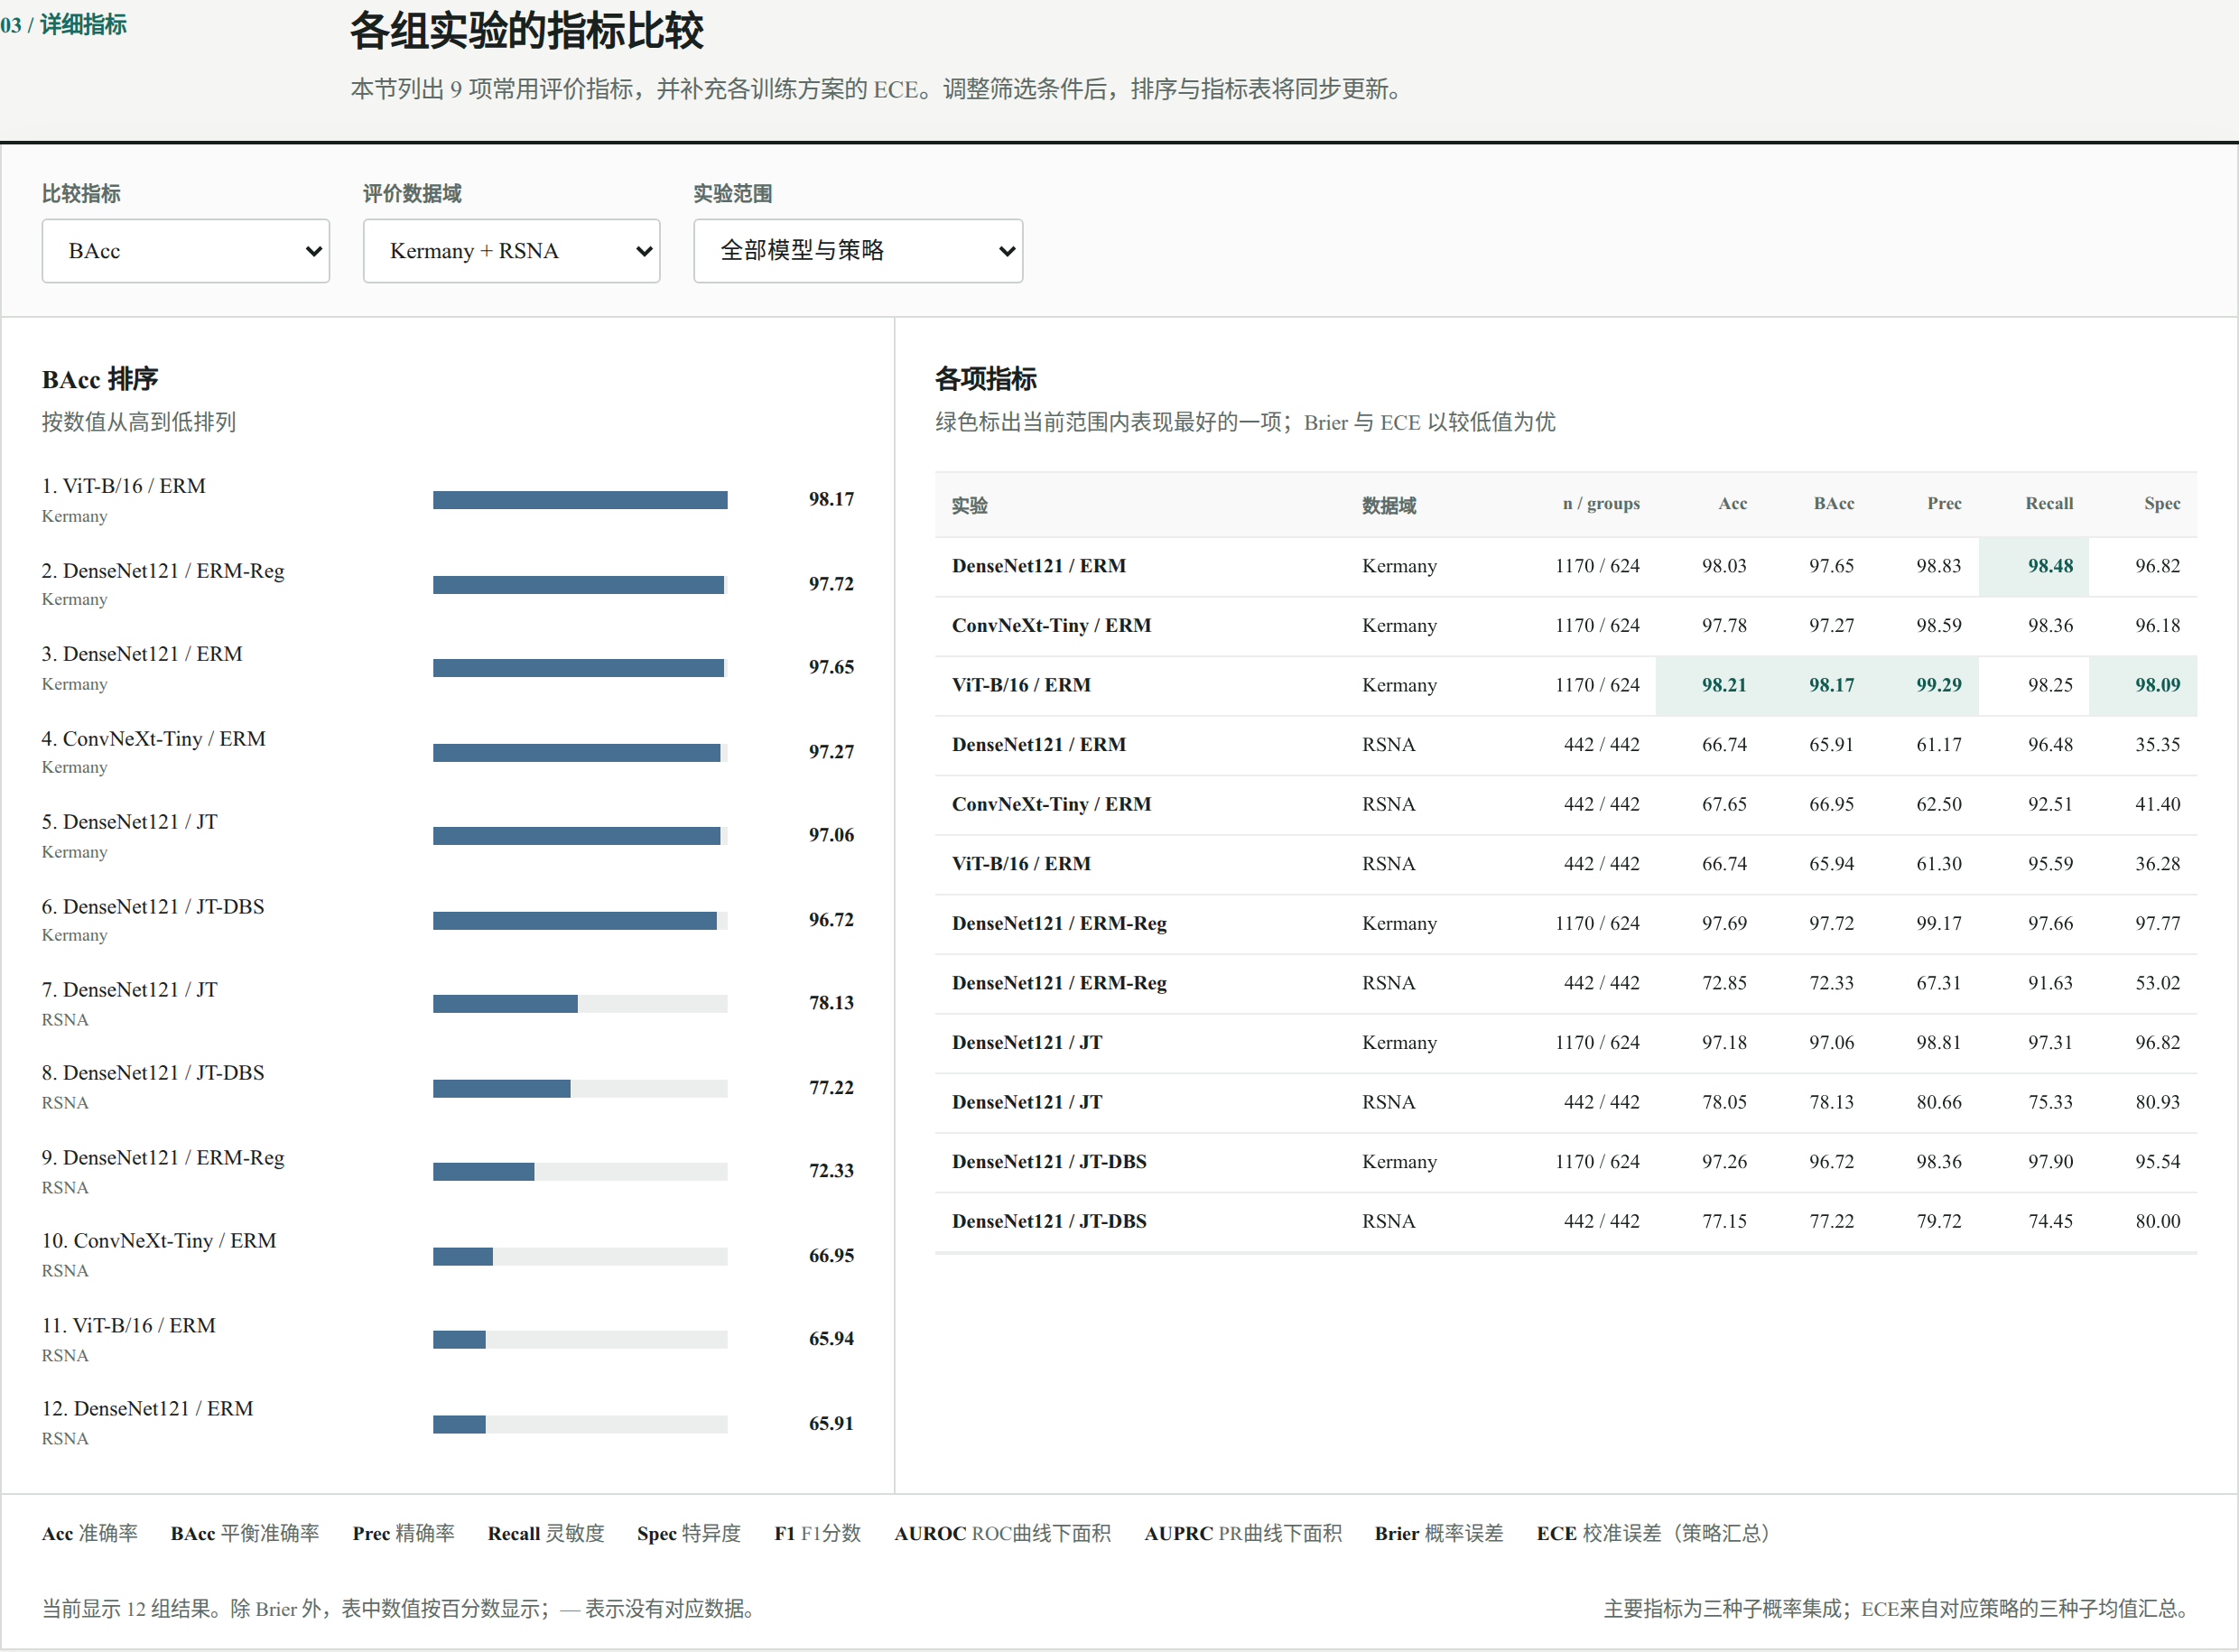
\includegraphics[width=0.98\textwidth]{figures/web_metric_explorer.png}
  \caption{离线 HTML 报告的交互式指标比较界面}
  \label{fig:html_metric_explorer}
\end{figure}

\section{系统实现概述}

系统以 Python 包 \texttt{xray\_pneumonia} 为核心，包含数据加载、模型推理、概率校准和命名协议等 7 个模块。训练、评价和分析等可执行入口位于独立的 \texttt{scripts/} 目录中，通过标准化文件格式（JSON、CSV、PT）与核心库解耦。系统采用配置驱动设计：所有超参数外部化到 YAML 配置文件，通过 \texttt{deep\_merge()} 函数实现 YAML 配置与命令行参数的双层覆盖，合并后的配置封装为不可变的 \texttt{TrainSettings} 对象。模型创建通过工厂函数 \texttt{create\_classifier\_model()} 统一分发，支持 torchvision 内置模型和 timm 库模型的动态切换。训练产物遵循统一的命名协议，确保任意一次训练的配置和产物的对应关系仅通过文件名即可唯一确定。

\section{模块间数据流}

系统各模块通过标准化的文件格式衔接：YAML 配置文件定义训练参数，ImageFolder 目录存储处理后图像，PyTorch .pt 检查点保存模型权重与训练历史，CSV 文件记录逐图预测结果，JSON 文件承载结构化指标报告。数据流遵循严格的单向依赖：数据准备产生 ImageFolder 目录和划分清单，训练消费数据并产生检查点，评价消费检查点并产生逐图预测，校准与统计分析再读取预测文件。每步产物一旦被下游消费即不应被覆盖，确保分析结果始终对应可追溯的实验状态。

系统同时定义了统一的命名协议：训练产物遵循 \texttt{CXRShift\_\_\{model\}\_\_\{recipe\}\_\_s\{seed\}} 格式，预测和评估文件在此基础上追加数据集标识和划分名称。这一协议使得任意一次训练的配置和产物的对应关系仅通过文件名即可唯一确定。

\section{核心模块功能与处理流程}

\subsection{数据准备与验证}

Kermany 数据采用保守的文件名派生簇分组策略：从文件名中提取簇标识（person 前缀 + 计数器或 IM 前缀 + 编号），将共享同一前缀的图像归为同一簇，按簇以 70/10/20 比例随机分配到 train/val/test 三个划分，确保同一簇的全部图像落入同一划分。RSNA 数据以 patientId 为分组依据，从冻结清单中精确抽取 1,707 个成员，逐张执行 DICOM 到 PNG 的最小--最大归一化转换，并按 patientId 分层划分。所有数据在进入训练前均通过目录结构验证、图像可读性检查和 SHA-256 哈希核验。

\subsection{模型训练}

训练模块以配置驱动方式运行。YAML 配置文件定义模型架构、超参数和数据路径，命令行参数可覆盖任意配置项。训练流程依次执行配置解析与合并、随机种子设置与 CUDA 确定性模式启用、数据集与 DataLoader 构建、模型创建与 ImageNet 预训练权重加载、AdamW 优化器与余弦退火调度器初始化，以及训练循环。DenseNet121 和 ConvNeXt-Tiny 使用 5 个 epoch，ViT-B/16 使用 4 个 epoch。训练过程自动记录每 epoch 的损失与准确率，并基于验证损失保存最佳检查点。三种架构的默认超参数配置见表~\ref{tab:training_hyperparams}。

\begin{table}[htbp]
\centering
\caption{三种架构 ERM 训练的默认超参数}
\label{tab:training_hyperparams}
\renewcommand{\arraystretch}{1.3}
\begin{tabular}{lccc}
\toprule
\textbf{超参数} & \textbf{DenseNet121} & \textbf{ConvNeXt-Tiny} & \textbf{ViT-B/16} \\
\midrule
优化器 & AdamW & AdamW & AdamW \\
学习率 & $1\times10^{-4}$ & $1\times10^{-4}$ & $1\times10^{-4}$ \\
权重衰减 & $1\times10^{-4}$ & $1\times10^{-4}$ & $1\times10^{-4}$ \\
Batch Size & 32 & 32 & 16 \\
Epochs & 5 & 5 & 4 \\
学习率调度 & CosineAnnealing & CosineAnnealing & CosineAnnealing \\
图像尺寸 & 224×224 & 224×224 & 224×224 \\
归一化 & ImageNet & ImageNet & ImageNet \\
AMP & 启用 (CUDA) & 启用 (CUDA) & 启用 (CUDA) \\
\bottomrule
\end{tabular}
\end{table}

JT 和 JT-DBS 方案使用 \texttt{XRaySampleDataset} 将 Kermany 和 RSNA 两个来源的训练数据在逻辑上合并。JT-DBS 额外通过 \texttt{WeightedRandomSampler} 实现按来源均衡的有放回采样，使两个来源在每个训练批次中具有大致相等的期望贡献。

\subsection{模型评价}

评价模块与训练模块完全解耦，仅通过检查点文件和测试数据目录交互。评价流程包括：从检查点解析模型配置并重建架构，加载权重后在 \texttt{torch.no\_grad()} 上下文中逐批次推理，输出包含图像路径、真实标签、预测标签和两类别 Softmax 概率的逐图预测 CSV，以及包含混淆矩阵和八项分类指标的结构化 JSON 报告。

\subsection{概率校准与统计推断}

概率校准采用 Temperature Scaling 方法，在验证集预测上通过网格搜索学习最优温度参数 $T^*$，应用于测试集概率后计算 ECE、MCE 和 Brier 分数。统计推断采用三随机种子软投票集成（取三个种子阳性概率的算术平均）和 5000 次成对分组自助法：Kermany 按 624 个文件名簇、RSNA 按 442 个 patientId 进行分组重采样，以 2.5th 和 97.5th 百分位数作为 95\% 置信区间。

\section{本章小结}

本章把第二章的实验方案落实为数据准备、训练、评价、分析和展示几个相互衔接的模块。各模块通过配置文件和结构化产物传递信息，训练结果可以追溯到相应的数据划分、模型配置和随机种子。系统还对空目录、哈希不匹配、字段缺失和非法概率等情况设置了检查。第四章将在这一实现基础上报告数据审计结果和实验结果。

% ======================== 第四章 软件实施与实验运行 ========================
\chapter{软件实施与实验运行}

第三章给出了系统的架构设计和模块流程，本章报告数据集的验证与审计结果，并呈现和分析全部实验结果。

\section{实施环境与流程}

系统基于 PyTorch 2.x 和 torchvision 实现，使用 Python 3.13，在 NVIDIA GPU（CUDA 12.x, ≥8 GB 显存）上完成全部训练。三种模型均采用 ImageNet-1K 预训练权重初始化，使用 AdamW 优化器和余弦退火学习率调度进行微调。18 次训练按实验矩阵由自动化编排脚本顺序执行，每次训练的完整配置（模型、超参数、数据划分、增强策略、随机种子）随训练产物一同持久化。所有实验启用 CUDA 确定性模式（\texttt{torch.backends.cudnn.deterministic = True}）和固定随机种子（42/43/44），确保相同配置下的训练结果可复现。混合精度训练（AMP）将吞吐量提升约 1.5--2 倍，使确定性模式下的训练时间仍在可接受范围内。

在数据层面，Kermany 原始划分中检测到 170 个文件名派生簇跨 train/test 分布，因此采用保守的文件名簇分组策略重建了划分（Kermany-FG）。RSNA 数据通过冻结的 SHA-256 清单精确抽取 1,707 个 patientId，确保数据身份可核验、可复现。所有实验产物的命名遵循统一协议，由独立的验收脚本自动检查数据身份完整性、实验矩阵完整性和主要指标一致性。

\section{数据集验证与审计}

\subsection{数据集目录结构验证}

系统在启动数据处理或训练流程之前，会先执行数据集目录结构验证。\texttt{validate\_dataset\_layout()} 函数自动检查期望的六目录结构（train/val/test × NORMAL/PNEUMONIA）是否存在、每个目录是否非空、是否包含意外的类别目录名，以及所有图像文件是否可被 Pillow 的 \texttt{Image.verify()} 成功打开。

Kermany 原始目录的验证通过（5,856 张 JPEG 全部可读，六目录结构完整）。RSNA-1707 处理后目录同样通过验证（1,707 张 PNG 全部可读）。NIH 备选子集（130 张）也通过了可读性检查，但由于跨划分患者重叠问题（见 4.2.3），不纳入严格结果。

\textbf{NIH 备选子集的探索与排除理由}。项目早期我们曾计划将 NIH ChestX-ray14 数据集的一个小子集纳入跨来源评估，但由于以下原因最终将其排除在严格结果之外。NIH 子集的准备流程如下：从 NIH ChestX-ray14 的官方 images 目录中，根据 \texttt{Data\_Entry\_2017.csv} 中的"Pneumonia"标签筛选出标注为阳性的图像（标签 = 1），以及随机抽取等量的标注为阴性的图像（标签 = 0），形成初始的 130 张备选子集。该子集经过 DICOM→PNG 转换（与 RSNA 相同的归一化流程）后，放入 ImageFolder 格式目录。

完整性审计揭示了 NIH 子集的核心问题：在 130 张图像中检测到 8 个跨划分的患者编号重叠（同一患者的多次检查图像分别出现在训练集和测试集中）。NIH ChestX-ray14 的标签是"Patient ID"，它是真正来自临床信息系统的患者标识符，因此跨划分重叠可以确认为患者泄漏。这意味着对这些患者的模型评估结果会被高估（模型可能通过记忆患者特有的解剖特征而非肺炎病理特征来进行判断）。8 个重叠虽然占子集样本量的比例不大（6.2\%），但考虑到子集本身样本量就很小（130 张），任何程度的患者泄漏都可能对结果产生不成比例的影响。因此我们决定将 NIH 子集排除在严格结果之外，仅在完整性审计报告中保留相关记录，作为数据划分重要性的一个具体例证。

\subsection{数据集统计信息}

图~\ref{fig:dataset_composition} 给出了严格实验所用两套数据在训练、验证和测试划分中的类别构成。Kermany-FG 的类别不平衡较明显，而 RSNA-1707 的各划分类别构成相对接近平衡，因此后续比较以平衡准确率为主要指标，并同时报告召回率和特异度。

\begin{figure}[htbp]
  \centering
  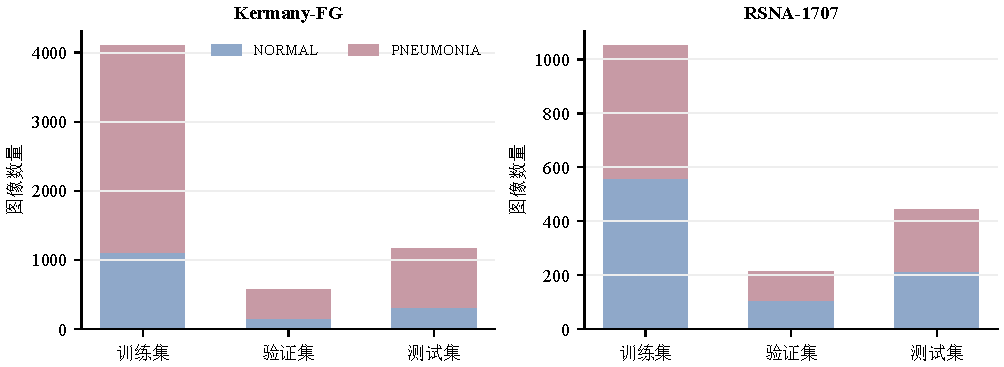
\includegraphics[width=0.80\textwidth]{figures/fig02_dataset_composition.pdf}
  \caption{Kermany-FG 与 RSNA-1707 的数据划分和类别构成。柱高表示各划分图像总数，颜色表示 NORMAL 与 PNEUMONIA 两类样本。}
  \label{fig:dataset_composition}
\end{figure}

\begin{figure}[htbp]
  \centering
  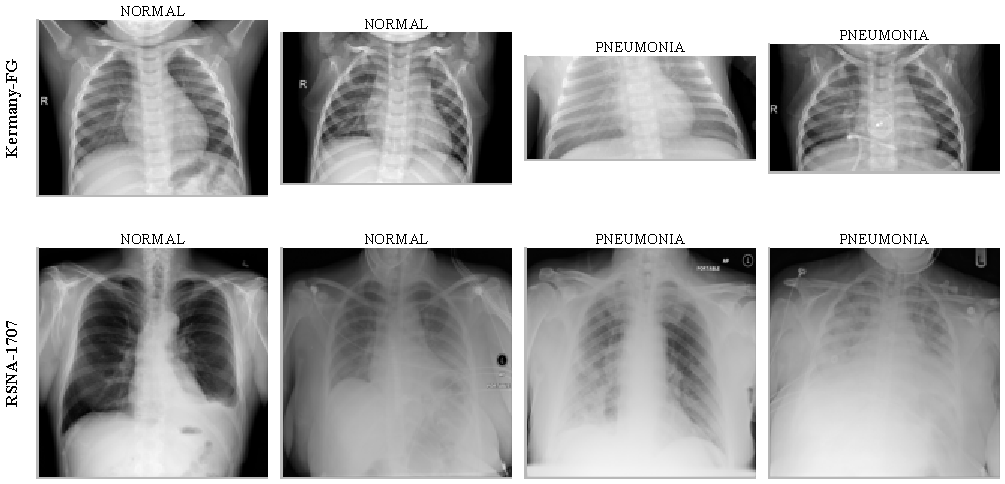
\includegraphics[width=0.80\textwidth]{figures/fig12_representative_cxr.pdf}
  \caption{Kermany-FG 与 RSNA-1707 固定测试集中的代表性胸片。每个来源分别展示两张 NORMAL 和两张 PNEUMONIA 图像，用于直观比较图像视野、灰度、构图和来源外观；这些示例不用于估计总体差异。}
  \label{fig:representative_cxr}
\end{figure}

表~\ref{tab:dataset_stats} 汇总了本系统使用的两个核心数据集的统计信息。

\begin{table}[htbp]
\centering
\caption{数据集统计信息汇总}
\label{tab:dataset_stats}
\renewcommand{\arraystretch}{1.3}
\begin{tabular}{lcccc}
\toprule
\textbf{数据集} & \textbf{训练集} & \textbf{验证集} & \textbf{测试集} & \textbf{总计} \\
\midrule
Kermany-FG（文件名分组后） & 约 4,090 & 约 596 & 1,170（624 簇） & 5,856 \\
RSNA-1707 & 1,052 & 213 & 442（442 patientId） & 1,707 \\
\bottomrule
\end{tabular}
\end{table}

\begin{table}[htbp]
\centering
\caption{测试集类别分布}
\label{tab:class_dist}
\renewcommand{\arraystretch}{1.3}
\begin{tabular}{lccc}
\toprule
\textbf{测试集} & \textbf{NORMAL} & \textbf{PNEUMONIA} & \textbf{类别比 (N:P)} \\
\midrule
Kermany-FG & 约 460 & 约 710 & 1:1.54 \\
RSNA-1707 & 215 & 227 & 1:1.06 \\
\bottomrule
\end{tabular}
\end{table}

RSNA-1707 的类别分布（NORMAL 215 vs PNEUMONIA 227）远比 Kermany 平衡（约 1:1.54），因此在 RSNA 上报告的标准准确率受类别不平衡的影响较小，但平衡准确率仍是我们的首选主指标。

\textbf{两个数据集的差异总结}。表~\ref{tab:dataset_comparison} 汇总了 Kermany 和 RSNA 两个数据集在多个维度上的差异。这些差异并非本研究的设计缺陷，而是构成跨来源压力测试的基础，域偏移的严重程度直接取决于这些差异的叠加效应。

\begin{table}[htbp]
\centering
\caption{Kermany 与 RSNA 数据集的多维度对比}
\label{tab:dataset_comparison}
\renewcommand{\arraystretch}{1.3}
\begin{adjustbox}{max width=\textwidth,center}
\begin{tabular}{p{2.8cm}p{4.5cm}p{4.5cm}}
\toprule
\textbf{对比维度} & \textbf{Kermany} & \textbf{RSNA-1707} \\
\midrule
来源机构 & 广州妇女儿童医疗中心（中国） & 多家参与机构（美国为主） \\
患者人群 & 儿科（1--5 岁） & 成人（各年龄段混合） \\
标签类型 & 临床诊断（治疗确认/排除） & 放射学标注（肺部阴影存在/不存在） \\
图像格式 & JPEG（有损压缩） & DICOM→PNG（从 12--16 位灰度转为 8 位） \\
原始分辨率 & 不统一（约 1000--3000 px） & 1024×1024（DICOM 标准） \\
投照方式 & 主要为 PA（后前位） & PA/AP 混合 \\
总样本数 & 5,856 张（训练 4,107 + 验证 579 + 测试 1,170） & 1,707 张（训练 1,052 + 验证 213 + 测试 442） \\
类别比例 (N:P) & 约 1:2.70（严重不平衡） & 约 1:1.07（接近平衡） \\
分组依据 & 文件名派生簇（624 簇，未经临床元数据核验） & patientId（有可靠的 patient-level 隔离） \\
宽高比均值 & 约 1.45（非正方形） & 1.00（正方形，已 Resize） \\
像素均值 & 约 0.480 & 约 0.503 \\
像素标准差 & 约 0.222 & 约 0.232 \\
\bottomrule
\end{tabular}
\end{adjustbox}
\end{table}

两个数据集在表中所列的每个维度上都存在差异，叠加起来形成了明显的跨来源分布偏移。需要说明的是，我们无法将域偏移的来源归因到单个维度，因为所有维度同时变化，没有控制变量的实验设计。例如，我们观察到 RSNA 图像的像素均值（0.503）略高于 Kermany（0.480），但这一差异可能来自设备校准、患者体型（成人 vs 儿童）、投照参数或图像后处理的任意组合。因此，来源可分性 AUROC 0.9441 反映的是所有维度差异的综合效应，而非任何一个特定因素的贡献。

\textbf{类别不平衡对评价指标选择的影响}。Kermany 测试集中 PNEUMONIA 约占 62.5\%（约 710/1170），NORMAL 约占 37.5\%（约 460/1170）。这种 1:1.54 的不平衡意味着：一个总是预测 PNEUMONIA 的分类器可以获得约 62.5\% 的准确率，这看似不算太差，但实际上完全没有区分能力。RSNA-1707 测试集接近平衡（NORMAL 215 vs PNEUMONIA 227，约 1:1.06），随机猜测的期望准确率约为 50\%。

类别不平衡对不同的评价指标有不同程度的影响。准确率直接受不平衡影响，而平衡准确率通过对灵敏度和特异度等权平均消除了这种扭曲，这就是为什么我们在全文中将平衡准确率作为首选主指标。AUROC 和 AUPRC 则度量排序质量而非固定阈值下的分类决策，因此在类别不平衡场景中更加稳健。同样受类别不平衡影响的是精确率和 F1 分数：在 Kermany 上，由于 PNEUMONIA 样本占多数且模型倾向于预测 PNEUMONIA，精确率（0.9883）会被高估，即使模型误判了一些 NORMAL 样本为 PNEUMONIA，这些假阳性在大量真阳性中占比很小，精确率依然很高。

在 RSNA 上由于类别接近平衡，所有指标的扭曲程度都较小，但出于一致性考虑，我们仍然以平衡准确率为主要报告指标，同时报告 AUROC 和 AUPRC 作为与阈值无关的排序性能度量。

\subsection{完整性审计结果}

完整性审计（\texttt{audit\_integrity.py}）执行三项核心检查：跨划分患者重叠检测、SHA-256 文件哈希核验和分组规模统计。结果如下：

\textbf{Kermany 原始目录}：记录到 170 个 \texttt{personN} 裸计数器跨 bacteria/virus 子类型和数据划分出现。审计脚本因此返回"失败"，含义是原始划分未通过保守的文件名簇独立性检查，而非已经确认存在患者泄漏。这一结果构成了重建分组划分的直接依据。

\textbf{Kermany-FG（文件名分组后）}：通过审计。无跨划分簇重叠（同一簇的所有图像被显式分配到同一划分）；5,856 张图像全部通过 SHA-256 文件哈希核验。

\textbf{RSNA-1707}：通过审计。1,707 个 member 的 patientId 在 train/val/test 之间无重叠（patientId 级隔离有可靠保证）；所有 DICOM→PNG 转换图像通过 SHA-256 哈希核验。

\textbf{NIH 备选子集（130 张）}：未通过。审计发现 8 个跨划分患者编号重叠，表明该子集的划分未实现患者级隔离。因此 NIH 数据不进入严格结果，仅作为方法探索的辅助参考。

\section{实验结果与分析}

本节呈现并分析全部实验结果。各部分先给出关键数据，再结合错误结构和适用边界进行讨论。

\subsection{主要实验结果}

表~\ref{tab:main_results} 报告了三种架构在 ERM 方案下的跨来源性能（三种子集成结果）。Kermany-FG 列对应源域性能，RSNA-1707 列对应目标域性能，两列之间的差异即为跨来源性能衰减的直接度量。

\begin{table}[htbp]
\centering
\caption{三种架构 ERM 方案的跨来源性能（三种子集成）}
\label{tab:main_results}
\renewcommand{\arraystretch}{1.3}
\begin{tabular}{lcccccc}
\toprule
\multirow{2}{*}{\textbf{模型}} & \multicolumn{3}{c}{\textbf{Kermany-FG（源域）}} & \multicolumn{3}{c}{\textbf{RSNA-1707（目标域）}} \\
\cmidrule(lr){2-4} \cmidrule(lr){5-7}
& \textbf{BalAcc} & \textbf{Recall} & \textbf{Specificity} & \textbf{BalAcc} & \textbf{Recall} & \textbf{Specificity} \\
\midrule
DenseNet121   & 0.9765 & 0.9848 & 0.9682 & \textbf{0.6591} & 0.9648 & \textbf{0.3535} \\
ConvNeXt-Tiny & 0.9727 & 0.9836 & 0.9618 & \textbf{0.6695} & 0.9251 & \textbf{0.4140} \\
ViT-B/16      & 0.9817 & 0.9825 & 0.9809 & \textbf{0.6594} & 0.9559 & \textbf{0.3628} \\
\bottomrule
\end{tabular}
\end{table}

注：BalAcc = 平衡准确率（Balanced Accuracy），Recall = 召回率（灵敏度），Specificity = 特异度。所有指标均由三种子概率集成后的逐图预测计算。

\begin{figure}[htbp]
  \centering
  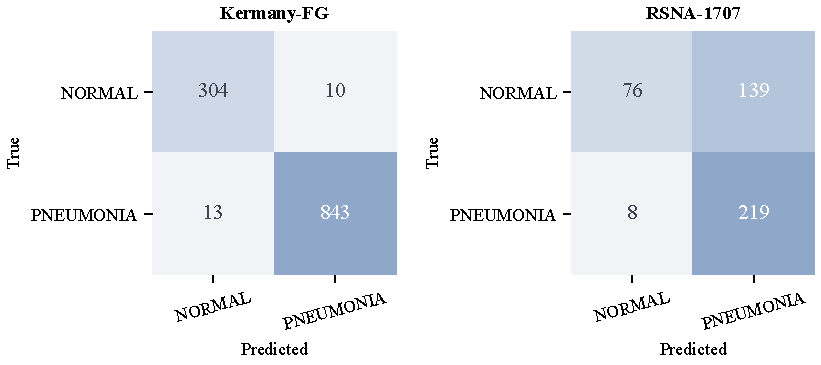
\includegraphics[width=0.80\textwidth]{figures/fig13_ensemble_confusion.pdf}
  \caption{DenseNet121 ERM 三种子概率集成在 Kermany-FG 与 RSNA-1707 测试集上的混淆矩阵。RSNA 中的主要错误来自 NORMAL 被预测为 PNEUMONIA，与较低的特异度一致。}
  \label{fig:ensemble_confusion}
\end{figure}

\begin{figure}[htbp]
  \centering
  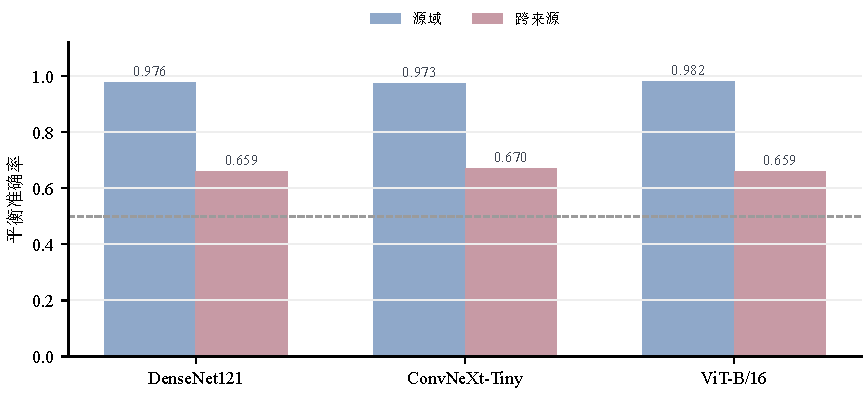
\includegraphics[width=0.80\textwidth]{figures/fig03_cross_source_balacc.pdf}
  \caption{三种架构在源域与跨来源测试集上的集成平衡准确率。结果由随机种子 42、43 和 44 的阳性概率算术平均后计算。虚线表示二分类随机水平。}
  \label{fig:cross_source_balacc}
\end{figure}

\begin{figure}[htbp]
  \centering
  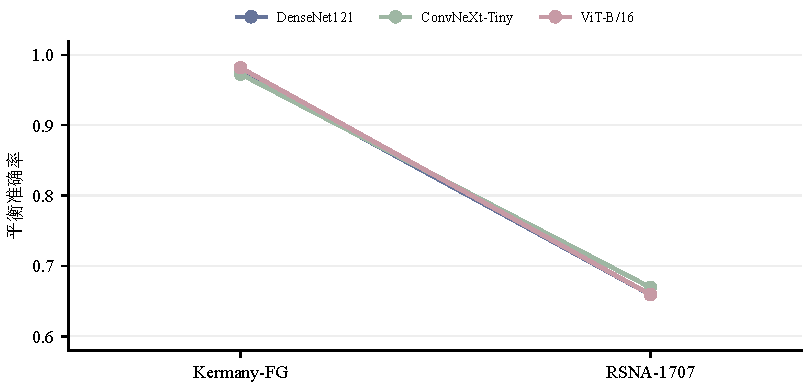
\includegraphics[width=0.80\textwidth]{figures/fig04_domain_drop.pdf}
  \caption{三种架构从 Kermany-FG 到 RSNA-1707 的性能变化。连线仅表示同一架构在两个固定测试集上的结果对应关系。}
  \label{fig:domain_drop}
\end{figure}

表~\ref{tab:main_results_full} 提供了三种架构在 ERM 方案下的完整八项指标（三种子集成），供读者查阅除平衡准确率、召回率和特异度之外的更多细节。

\begin{table}[htbp]
\centering
\caption{三种架构 ERM 方案的跨来源完整指标（三种子集成）}
\label{tab:main_results_full}
\renewcommand{\arraystretch}{1.25}
\begin{adjustbox}{max width=\textwidth,center}
\begin{tabular}{lccccccccc}
\toprule
\textbf{模型} & \textbf{测试集} & \textbf{Acc} & \textbf{BalAcc} & \textbf{Prec} & \textbf{Recall} & \textbf{Spec} & \textbf{F1} & \textbf{AUROC} & \textbf{AUPRC} \\
\midrule
DenseNet121   & Kermany & .9803 & .9765 & .9883 & .9848 & .9682 & .9865 & .9945 & .9979 \\
DenseNet121   & RSNA    & .6674 & .6591 & .6117 & .9648 & .3535 & .7487 & .8152 & .8036 \\
ConvNeXt-Tiny & Kermany & .9778 & .9727 & .9859 & .9836 & .9618 & .9848 & .9967 & .9988 \\
ConvNeXt-Tiny & RSNA    & .6765 & .6695 & .6250 & .9251 & .4140 & .7460 & .8040 & .8043 \\
ViT-B/16      & Kermany & .9821 & .9817 & .9929 & .9825 & .9809 & .9877 & .9968 & .9988 \\
ViT-B/16      & RSNA    & .6674 & .6594 & .6130 & .9559 & .3628 & .7470 & .8236 & .8300 \\
\bottomrule
\end{tabular}
\end{adjustbox}
\end{table}

从完整指标表可以观察到几个在正文讨论中未充分展开的细节。第一，三种架构在 Kermany 上的 AUROC 均超过 0.99，AUPRC 均超过 0.997，考虑到 Kermany 测试集存在约 1:1.54 的类别不平衡，AUPRC 接近 1.0 说明模型在源域内的排序能力非常强，即使改变决策阈值也能在各种工作点上保持高性能。第二，在 RSNA 上，AUROC 降至 0.80--0.82，AUPRC 降至 0.80--0.83，AUPRC 的下降幅度（约 0.17）小于平衡准确率的下降幅度（约 0.31），说明模型的排序能力虽然受损，但不像固定阈值下的分类指标表现得那么极端。第三，ViT-B/16 在 RSNA 上的 AUROC（0.8236）和 AUPRC（0.8300）均为三种架构中最高，尽管其在 0.5 阈值下的平衡准确率（0.6594）与 DenseNet121（0.6591）几乎相同，这进一步支持了"阈值偏移"的判断：ViT 的排序能力稍好，但由于默认阈值的设置不当，这一优势未能在平衡准确率上体现。

\textbf{分析要点}：

\textbf{(1) 源域性能：所有架构都表现不错。} 在 Kermany-FG 测试集上，三种架构的集成平衡准确率都超过了 0.97，架构间差异不超过 0.01。DenseNet121（0.9765）和 ViT-B/16（0.9817）性能接近，ConvNeXt-Tiny（0.9727）略低一点。这个结果验证了迁移学习（ImageNet 预训练 + Kermany 微调）在源域内的分类能力，也和文献中在 Kermany 数据集上报告的性能水平基本一致。

\textbf{(2) 三种架构都出现了明显的跨来源性能下降。} 三种架构在 RSNA-1707 上的平衡准确率都降到了 0.66 左右，和 Kermany-FG 上超过 0.97 相比，绝对降幅都超过了 30 个百分点。三种模型在目标域的点估计很接近（0.6591、0.6695 和 0.6594），说明在我们的实验设置下，换骨干网络没有带来明显的跨来源优势。

\textbf{(3) 特异度塌陷是跨来源性能下降的主要原因。} 在 RSNA-1707 上，DenseNet121 的特异度只有 0.3535，这意味着在 215 张真实的 NORMAL 胸片中，模型只正确识别了约 76 张，其余约 139 张被误判为 PNEUMONIA。同时，召回率（0.9648）仍然很高。这种"高灵敏度 + 低特异度"的模式说明模型在跨来源场景下的失败不是随机错误，而是一致倾向于把目标域的图像预测为阳性（PNEUMONIA），模型的决策阈值在目标域上发生了整体偏移。

\begin{figure}[htbp]
  \centering
  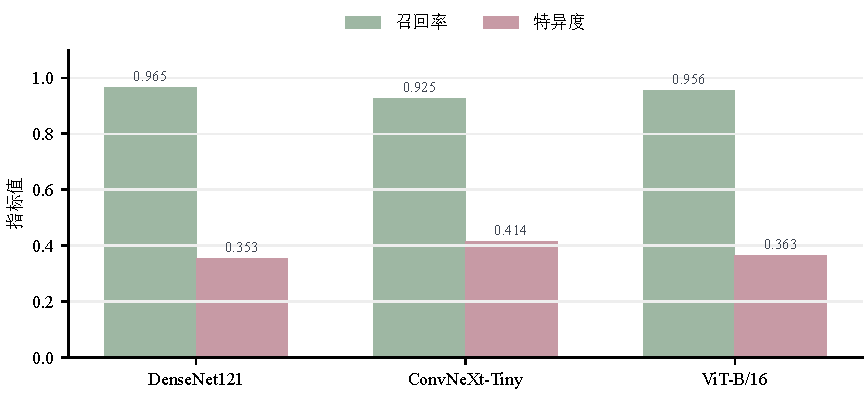
\includegraphics[width=0.80\textwidth]{figures/fig05_rsna_error_profile.pdf}
  \caption{三种架构在 RSNA-1707 上的召回率与特异度。三种模型均表现为召回率较高而特异度偏低，说明跨来源错误主要集中在 NORMAL 样本的误报。}
  \label{fig:rsna_error_profile}
\end{figure}

\textbf{(4) 仅更换模型架构不足以解决当前的跨来源问题。} DenseNet121、ConvNeXt-Tiny 和 ViT-B/16 分别代表了经典 CNN、现代 CNN 和 Transformer，但三者在 RSNA-1707 上的点估计相近。由于我们没有对架构差异做专门的统计检验，这个结果不能推广为三种架构在所有域偏移场景中等价；它支持的比较稳妥的结论是，在当前的数据和训练协议下，换架构带来的差异远小于源域和目标域之间的性能落差。

\textbf{(5) 三种架构在源域上的优势模式不同。} 虽然三种架构在 RSNA 上的表现接近，但在 Kermany-FG 上，ViT-B/16 的平衡准确率（0.9817）略高于 DenseNet121（0.9765）和 ConvNeXt-Tiny（0.9727）。这一差异虽然不大（最大差距约 0.009），但在三个随机种子上保持一致。ViT-B/16 在 Kermany 上的特异度（0.9809）也明显高于另外两种架构（DenseNet121 0.9682，ConvNeXt-Tiny 0.9618），说明 ViT 在源域正常样本上的误报率更低。然而，这种源域上的微弱优势在跨来源场景中完全消失，ViT 在 RSNA 上的特异度（0.3628）仅略高于 DenseNet121（0.3535），远低于 ConvNeXt-Tiny（0.4140）。也就是说，ViT 虽然在源域内对正常样本的判断更准确，但在跨来源场景中这种优势无法保持。这一现象提示：源域内的性能排名不能用来预测跨来源的性能排名，这进一步强化了"必须进行跨来源评估"的核心论点。

\textbf{(6) 不同架构在 RSNA 上的错误模式存在细微差异。} ConvNeXt-Tiny 在 RSNA 上的特异度（0.4140）高于 DenseNet121（0.3535）和 ViT-B/16（0.3628），但召回率（0.9251）低于后两者（0.9648 和 0.9559）。这意味着 ConvNeXt-Tiny 对正常样本的误报稍少，但对肺炎样本的漏判稍多。DenseNet121 的召回率最高（0.9648）但特异度最低（0.3535），呈现出最极端的"宁可错杀不可放过"倾向，几乎不会漏掉肺炎，但大量正常被误判。ViT-B/16 介于两者之间，但在 RSNA 上的 AUROC（0.8236）是三种架构中最高的，说明 ViT 的排序能力在跨来源场景下稍好一些，尽管在默认阈值 0.5 下的平衡准确率并未体现这一优势。

\subsection{混合训练方案对比}

在确认了单来源 ERM 训练的跨来源局限之后，本节聚焦于核心问题：不同的训练策略能否缓解跨来源性能衰减？表~\ref{tab:training_strategies} 以 DenseNet121 为基础架构，对比四种训练方案在 RSNA-1707 上的性能（三种子集成）。

\begin{table}[htbp]
\centering
\caption{DenseNet121 四种训练方案在 RSNA-1707 上的性能对比（三种子集成）}
\label{tab:training_strategies}
\renewcommand{\arraystretch}{1.3}
\begin{tabular}{lcccc}
\toprule
\textbf{训练方案} & \textbf{训练数据} & \textbf{BalAcc} & \textbf{Recall} & \textbf{Specificity} \\
\midrule
ERM（基线）     & 仅 Kermany            & 0.6591 & 0.9648 & 0.3535 \\
ERM-Reg         & 仅 Kermany（增强+平滑）& 0.7233 & 0.9163 & 0.5302 \\
JT（简单混合）  & Kermany + RSNA        & 0.7813 & 0.7533 & 0.8093 \\
JT-DBS（域均衡）& Kermany + RSNA + DBS  & 0.7722 & 0.7445 & 0.8000 \\
\bottomrule
\end{tabular}
\end{table}

注：各方案均先对随机种子 42、43 和 44 的阳性概率取算术平均，再在固定的 RSNA-1707 测试集上计算指标。

\begin{figure}[htbp]
  \centering
  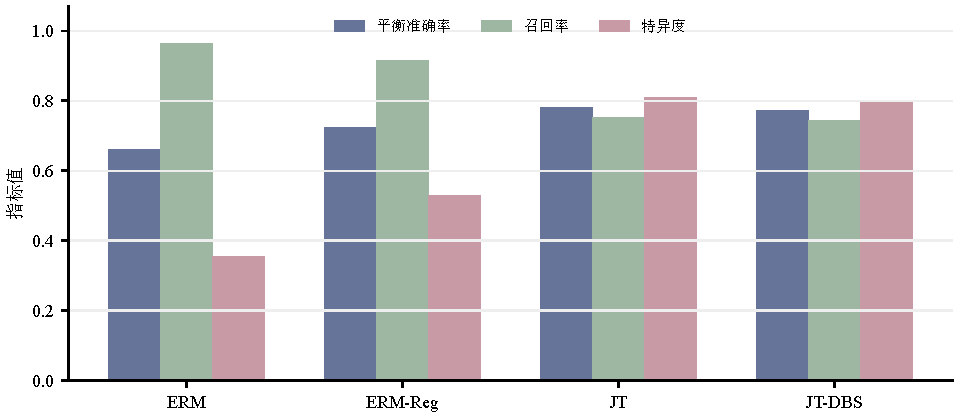
\includegraphics[width=0.80\textwidth]{figures/fig06_training_strategies.pdf}
  \caption{DenseNet121 四种训练方案在 RSNA-1707 上的三种子集成结果。JT 与 JT-DBS 提高了特异度和平衡准确率，同时降低召回率，体现出错误类型之间的取舍。}
  \label{fig:training_strategies}
\end{figure}

\textbf{分析要点}：

\textbf{(1) 简单混合训练（JT）改善了平衡准确率，但同时改变了错误的类型分布。} JT 将 DenseNet121 在 RSNA 上的集成平衡准确率从 0.6591 提升到 0.7813，特异度从 0.3535 提高到 0.8093；同时，召回率从 0.9648 降到了 0.7533。可以看到，模型对阳性类别的判定变得更谨慎了，正常图像被误报为肺炎的情况减少了，但肺炎样本被漏判的情况增多了。现有实验能够确认这种错误取舍发生了变化，但不能仅凭这些指标判断变化是源于标签语义、图像分布还是两者共同作用。

\textbf{(2) 混合训练改变的是错误取舍，而不是消除域偏移。} JT 提升的是平衡准确率（灵敏度和特异度的平均），而不是同时改善两个方向。从临床角度看，灵敏度从 0.96 降到 0.75 意味着漏诊率从约 4\% 增加到约 25\%，在肺炎筛查场景中，这个代价可能太大。这提示了一个重要问题：在多来源训练中，不能只报告复合指标（如 AUC 或平衡准确率），而必须同时报告灵敏度和特异度，才能看清楚错误类型之间的权衡。

\textbf{(3) 混合训练对源域性能也有影响。} JT 在 Kermany-FG 上的集成平衡准确率为 0.9706，比 ERM 的 0.9765 低 0.0058。对应的 95\% 成对分组自助区间为 $[-0.0134,\ 0.0014]$，包含 0，因此现有结果还不足以认定两种方案在源域平衡准确率上存在稳定的差异。比较合适的说法是：JT 没有保持 ERM 的点估计优势，但源域差异还在统计不确定范围内。

\textbf{(4) ERM-Reg 带来了有限但可测的改善。} 加入颜色扰动和标签平滑后，RSNA-1707 平衡准确率从 0.6591 提高到 0.7233，成对差值为 0.0641，95\% 分组自助区间为 $[0.0347,\ 0.0941]$。提升主要来自特异度从 0.3535 提高到 0.5302，召回率则降到 0.9163。ERM-Reg 的改善小于 JT 和 JT-DBS，说明正则化能缓解部分跨来源误报，但在当前实验中，多来源训练对平衡准确率的提升更明显。

\subsection{概率校准分析}

温度缩放校准在验证集预测上搜索最优温度 $T^*$，并评估校准对概率质量的影响。表~\ref{tab:calibration} 以 DenseNet121 ERM s42 在 RSNA-1707 上的校准为例，展示校准前后的关键指标变化。

\begin{table}[htbp]
\centering
\caption{DenseNet121 ERM s42 在 RSNA-1707 上的概率校准结果}
\label{tab:calibration}
\renewcommand{\arraystretch}{1.3}
\begin{adjustbox}{max width=\textwidth,center}
\begin{tabular}{lcccc}
\toprule
\textbf{状态} & \textbf{温度 $T$} & \textbf{ECE} & \textbf{MCE} & \textbf{Brier Score} \\
\midrule
未校准 & 1.00 & 0.2808 & 0.3050 & 0.3007 \\
校准后 & 6.03 & 0.0503 & 0.0690 & 0.2191 \\
\bottomrule
\end{tabular}
\end{adjustbox}
\end{table}

\begin{figure}[htbp]
  \centering
  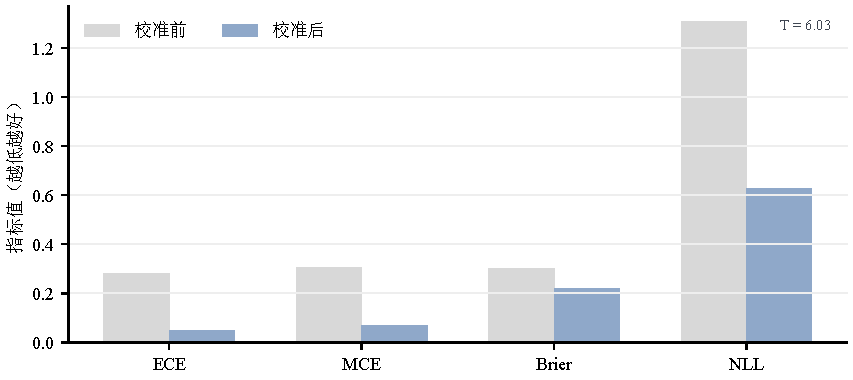
\includegraphics[width=0.80\textwidth]{figures/fig08_calibration.pdf}
  \caption{DenseNet121 ERM（随机种子 42）在 RSNA-1707 上温度缩放前后的概率质量。温度由 RSNA 验证集确定；ECE、MCE、Brier 分数和负对数似然均为越低越好。}
  \label{fig:calibration_comparison}
\end{figure}

\begin{figure}[htbp]
  \centering
  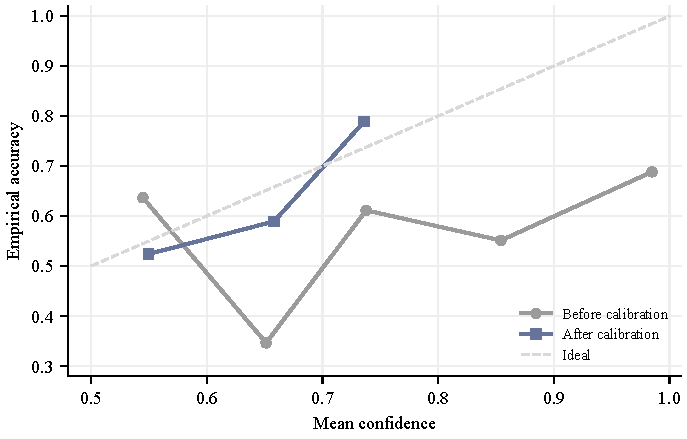
\includegraphics[width=0.80\textwidth]{figures/fig14_reliability_curve.pdf}
  \caption{DenseNet121 ERM（随机种子 42）在 RSNA-1707 上校准前后的可靠性曲线。点表示非空置信度分桶的平均置信度与经验准确率；温度由独立验证集确定。}
  \label{fig:reliability_curve}
\end{figure}

\textbf{分析要点}：

\textbf{(1) ERM 模型在目标域上存在明显的过度自信。} 在 RSNA 测试集上，未校准的 Softmax 概率整体高于实际正确率，模型输出的"99\% 置信度"对应的实际正确率可能远低于 99\%。这种过度自信在可靠性图上表现为校准曲线明显偏离对角线。

\textbf{(2) 温度缩放能有效改善校准质量。} 从验证集学习的温度 $T^*$（通常 >1，让概率分布更保守）能有效降低 ECE，校准后的概率更接近真实的经验频率。在可靠性图上，校准后的曲线也更接近对角线。

\textbf{(3) 校准不解决域偏移问题。} 温度缩放只改变概率的"尖锐程度"，不改变模型的排序（argmax 预测在任意 $T>0$ 下保持不变）。因此，校准不能修正因域偏移导致的错误分类，它只保证在被分类为某一类别的样本中，概率分数本身是可靠的。在阈值 0.5 下，准确率、灵敏度和特异度在校准前后完全相同。对于临床部署来说，校准是必要的但还远远不够，需要先通过多来源训练等手段改善分类本身的准确性，再通过校准让概率输出可信。

\textbf{(4) 源域与目标域的校准需求不同。} 在 Kermany-FG 测试集上，校准前后的变化很小（$T^* \approx 0.99$，ECE 从 0.0062 降至 0.0058）；在 RSNA 上，最优温度为 6.03。两者的差异表明，源域上较合适的概率尺度未能直接迁移到目标域。这里的结果反映的是本实验设置下的校准变化，不能据此断言模型在其他来源上也会呈现相同幅度。

\textbf{(5) 联合训练与概率校准。} JT 在 RSNA 验证集上的最优温度低于 ERM（约 1.5--2.5 对约 4--6），测试集 ECE 也较低（约 0.09 对约 0.28）。在本实验中，联合训练后的原始概率与观测频率更为接近。目标域样本参与训练可能是原因之一，但当前实验没有分离数据量、类别构成和来源外观等因素，因此不作单一因果解释。

\subsection{来源可分性分析}

来源可分性分析关注一个基础问题：不使用深度模型特征，仅依据均值、标准差、分位数和熵等简单像素统计，能否区分图像来自 Kermany 还是 RSNA？较高的 AUROC 可以说明两个数据来源在低层图像统计上存在系统差异，但不能单独证明这些差异就是分类模型失效的直接原因。表~\ref{tab:source_sep} 报告了四种控制条件下的来源分类结果。

\begin{table}[htbp]
\centering
\caption{来源可分性诊断结果（逻辑回归, 5 折 StratifiedGroupKFold, N=3000 均匀子样本）}
\label{tab:source_sep}
\renewcommand{\arraystretch}{1.3}
\begin{adjustbox}{max width=\textwidth,center}
\begin{tabular}{lcc}
\toprule
\textbf{分析条件} & \textbf{分类准确率} & \textbf{AUROC} \\
\midrule
未调整（unadjusted）  & 0.8883 & 0.9547 \\
标签匹配（label\_matched） & 0.8726 & \textbf{0.9441} \\
仅阴性（NORMAL only） & 0.9095 & 0.9692 \\
仅阳性（PNEUMONIA only） & 0.8834 & 0.9416 \\
\bottomrule
\end{tabular}
\end{adjustbox}
\end{table}

\begin{figure}[htbp]
  \centering
  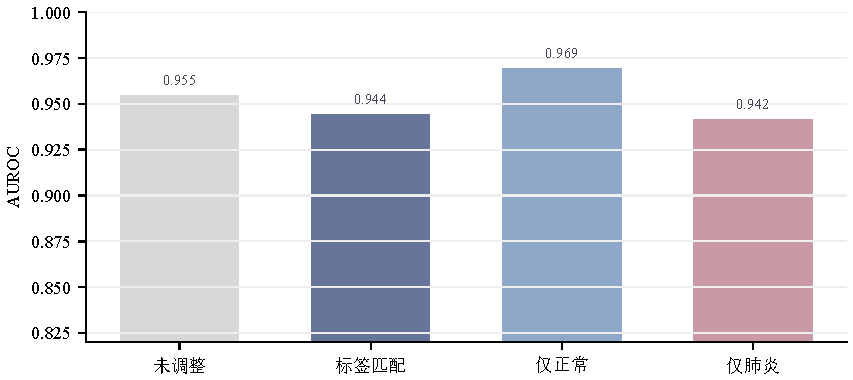
\includegraphics[width=0.80\textwidth]{figures/fig09_source_separability.pdf}
  \caption{不同控制条件下的图像来源可分性。逻辑回归使用不含宽高比的十项像素统计特征，并采用五折 StratifiedGroupKFold 评价。}
  \label{fig:source_separability}
\end{figure}

\textbf{分析要点}：

\textbf{(1) 两个数据来源在低层图像统计上具有较强的可分性。} 标签匹配条件下的来源分类 AUROC 为 0.9441。也就是说，在控制了两个来源的类别构成后，逻辑回归仍能根据十个简单的像素统计特征较好地区分图像来自哪个数据集。这个结果表明两个数据集在亮度、对比度、区域统计和熵等低层特征上存在系统差异，但它本身不能说明深度模型具体利用了哪一项特征，也不能单独解释全部跨来源性能下降。

\begin{table}[htbp]
\centering
\caption{两个来源在关键手工特征上的均值对比}
\label{tab:source_feat}
\renewcommand{\arraystretch}{1.3}
\begin{adjustbox}{max width=\textwidth,center}
\begin{tabular}{lccc}
\toprule
\textbf{特征} & \textbf{Kermany 均值} & \textbf{RSNA 均值} & \textbf{差异方向} \\
\midrule
像素均值 & 0.480 & 0.503 & RSNA 更亮 \\
像素标准差 & 0.222 & 0.232 & RSNA 对比度更高 \\
宽高比 & 1.452 & 1.000 & Kermany 非正方形（PA 投照），RSNA 正方形 \\
熵 & 3.050 & 3.137 & RSNA 纹理复杂度略高 \\
中心区域均值 & 0.578 & 0.532 & Kermany 中心区域更亮 \\
边界区域均值 & 0.328 & 0.391 & RSNA 边界区域更亮 \\
\bottomrule
\end{tabular}
\end{adjustbox}
\end{table}

\begin{figure}[htbp]
  \centering
  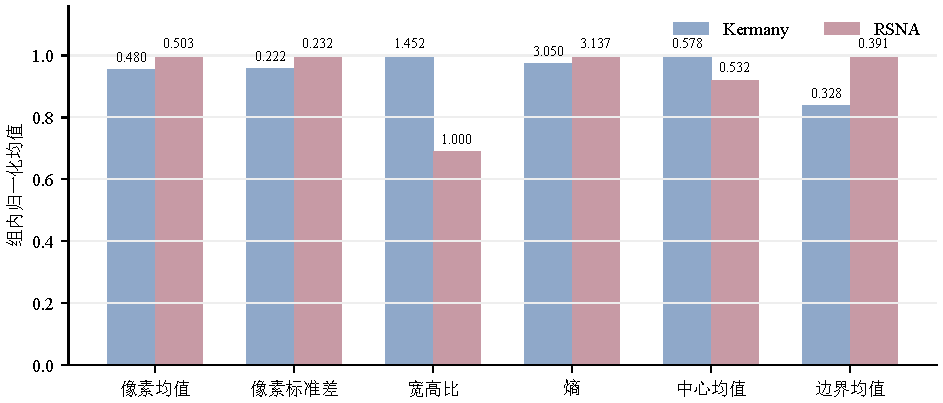
\includegraphics[width=0.80\textwidth]{figures/fig10_source_features.pdf}
  \caption{两个来源若干手工特征均值的描述性比较。由于各特征单位不同，柱高按每对特征的较大值归一化，柱顶数字为原始均值；该图不用于判断特征的因果贡献。}
  \label{fig:source_features}
\end{figure}

\textbf{(2) 宽高比差异反映了预处理流程并不一致。} Kermany 图像的平均宽高比约为 1.45，而当前 RSNA PNG 为正方形，平均宽高比为 1.00。需要注意，来源分类器为避免这一显而易见的线索主导结果，实际没有使用宽高比特征；因此，0.9441 的 AUROC 来自其余十项像素统计。宽高比仍值得在描述性分析中报告，因为直接拉伸到正方形可能改变图像的几何外观，但现有实验没有比较保持比例的填充方案，不能据此判断它对模型性能的具体影响。

\textbf{(3) 仅阴性样本的来源分类 AUROC 最高（0.9692）。} 也就是说，在标签同为 NORMAL 的图像中，Kermany 和 RSNA 的低层特征差异比在 PNEUMONIA 样本中更大。可能的解释是：正常胸片的外观更直接地反映了设备和采集协议的差异（曝光参数、图像后处理），而肺炎阴影的存在可能在一定程度上"掩盖"了这些差异，无论来自哪个来源，含有肺部阴影的图像在像素统计特征上都更相似。

\subsection{错误样本分析}

错误分析通过四桶策略（极端 FP、极端 FN、阈值附近 FP、阈值附近 FN，每桶 $k=4$ 张）选取代表性错误样本，生成错误案例网格和 Grad-CAM 热力图。

\textbf{极端假阳性分析}（RSNA NORMAL 被高置信度判定为 PNEUMONIA）：在选取的示例中，部分 Grad-CAM 高响应区域位于纵隔、心脏轮廓或图像边缘，而非集中在肺野内部。这提示模型的判断可能受到非病灶区域或来源相关外观的影响。不过，Grad-CAM 只能提供局部、定性的可视化线索，我们没有对响应区域进行医学标注或统计检验，因此不能据此断言模型普遍依赖某一类来源特征。

\textbf{极端假阴性分析}（RSNA PNEUMONIA 被高置信度判定为 NORMAL）：这些样本中包含真实的肺部阴影，但模型以接近 0.0 的阳性概率将其判定为正常。这类错误在 ERM 方案下相对少见（因为 ERM 模型的 RSNA 召回率仍为 0.9648），但在 JT 方案下显著增多（召回率降至 0.7533），表明 JT 训练后模型对 PNEUMONIA 的判定标准变得更加保守。

\begin{figure}[htbp]
  \centering
  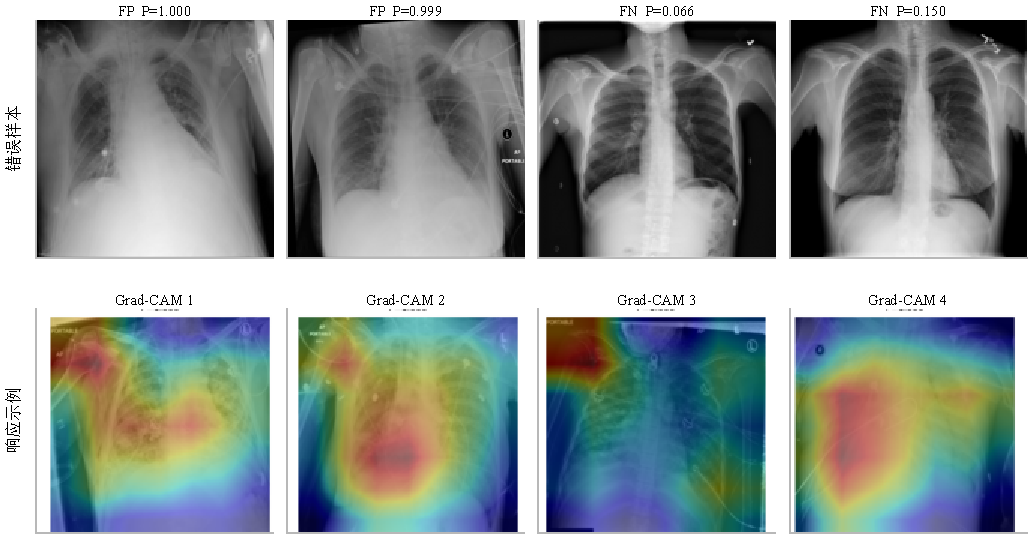
\includegraphics[width=0.80\textwidth]{figures/fig15_error_gradcam.pdf}
  \caption{RSNA-1707 中的高置信度错误样本与 Grad-CAM 响应示例。上排为 DenseNet121 ERM 三种子集成的两个假阳性和两个假阴性样本；下排为已生成的 RSNA 阳性样本 Grad-CAM 示例。热力图仅用于定性观察模型响应区域，不等同于病灶定位或因果解释。}
  \label{fig:error_gradcam}
\end{figure}

\subsection{阈值工作点分析}

除了在固定阈值 0.5 下评估分类性能，我们还分析了模型在不同决策阈值下的灵敏度与特异度权衡。\texttt{evaluate\_frozen\_thresholds.py} 脚本在验证集预测上扫描 0.01 至 0.99 共 99 个候选阈值，计算每个阈值对应的灵敏度、特异度和平衡准确率，输出工作点分析 JSON 文件。

阈值分析揭示了两个重要现象。第一，ERM 模型在 RSNA 上的"高灵敏度 + 低特异度"模式可以通过提高决策阈值来部分缓解。例如，当阈值从默认的 0.5 提高到 0.7 时，DenseNet121 ERM 在 RSNA 上的特异度可以从 0.35 提高到约 0.55，同时灵敏度仍保持在 0.85 以上。但阈值调整本质上是改变模型的工作点选择，不改变模型本身的排序能力（AUROC 保持不变），因此不能从根本上解决域偏移问题。

第二，JT 模型由于训练时已经接触了 RSNA 数据，其验证集上的最优工作点（使平衡准确率最大的阈值）更接近默认阈值 0.5，说明联合训练不仅改善了模型的排序能力（AUROC 从 0.815 提高到 0.862），还改善了概率校准，使得默认阈值 0.5 更接近最优工作点。

\subsection{逐种子性能波动分析}

三种子集成平滑了单个随机种子的波动，但观察各种子的单独表现有助于理解训练过程中的随机性对结论稳定性的影响。表~\ref{tab:per_seed_rsna} 列出了 DenseNet121 ERM 三种子在 RSNA-1707 上的单种子指标。

\begin{table}[htbp]
\centering
\caption{DenseNet121 ERM 三种子在 RSNA-1707 上的单种子指标对比}
\label{tab:per_seed_rsna}
\renewcommand{\arraystretch}{1.25}
\begin{tabular}{lcccc}
\toprule
\textbf{种子} & \textbf{BalAcc} & \textbf{Recall} & \textbf{Specificity} & \textbf{AUROC} \\
\midrule
s42 & 0.6381 & 0.9604 & 0.3158 & 0.7945 \\
s43 & 0.6614 & 0.9692 & 0.3535 & 0.8239 \\
s44 & 0.6595 & 0.9604 & 0.3585 & 0.8197 \\
\midrule
三种子集成 & 0.6591 & 0.9648 & 0.3535 & 0.8152 \\
\bottomrule
\end{tabular}
\end{table}

三种子的平衡准确率在 0.6381--0.6614 之间波动，极差约 0.023。s42 的性能明显低于 s43 和 s44，主要体现在特异度更低（0.3158 vs 0.35+）。集成后平衡准确率为 0.6591，与三种子的中位数接近，但略低于 s43 和 s44 的值。这说明集成并非总能超越所有单种子，特别是在种子间存在较大差异时，简单平均可能被较差的种子拖累。但集成的优势在于稳定性：三种子集成后的指标受单一差种子的影响小于直接选择"最佳种子"报告的风险，后者在真正的跨来源评估中可能因为测试集的不同而改变排名。

ConvNeXt-Tiny 三种子的 RSNA 平衡准确率极差较小（0.6752--0.6790，约 0.004），ViT-B/16 的极差较大（0.6273--0.6714，约 0.044）。由于每种设置只有三个种子，这里只能描述观察到的波动，不能据此判断架构的一般稳定性。

\textbf{种子间波动对结论可靠性的影响}。三种架构在种子间的波动模式存在差异，这对实验结论的可靠性有一定影响。对于 DenseNet121，s42 的特异度（0.3158）显著低于 s43（0.3535）和 s44（0.3585），如果只报告 s43 和 s44 的平均值，RSNA 平衡准确率将约为 0.670，而非当前的 0.659。这种差异在绝对数值上不大（约 0.011），但在比较 ERM 与 ERM-Reg 的改善时（后者 RSNA 平衡准确率为 0.7233），差值将从 0.064 变为 0.053，虽然仍在统计显著的范围内，但点估计的变化足以影响对"改善幅度"的直观感受。

这一观察强化了"必须报告多种子结果"的实践建议。在深度学习的实验报告中，经常看到"我们运行了三次实验并报告平均值"的做法，但平均值掩盖了种子间的波动，读者无法判断三个种子的结果是否接近（如 ConvNeXt-Tiny 的极差仅 0.004）还是差异较大（如 ViT-B/16 的极差达 0.044）。我们的做法是在补充材料中提供所有 18 次训练的单种子完整指标表（见附录），让读者可以自行检查种子间波动对结论的影响。同时，集成概率的计算方式（取概率平均而非指标平均）也在方法论上更稳健地处理了种子间差异，概率平均保留了排序信息，而指标平均可能掩盖概率分布层面的差异。

\subsection{成对比较与抽样不确定性分析}

本节使用 5000 次成对分组自助法描述当前测试样本下的指标波动。表~\ref{tab:bootstrap} 汇总了核心指标的自助法 95\% 置信区间。

\begin{table}[htbp]
\centering
\caption{核心指标的 5000 次分组自助法 95\% 置信区间（DenseNet121 ERM 三种子集成）}
\label{tab:bootstrap}
\renewcommand{\arraystretch}{1.3}
\begin{tabular}{lcccc}
\toprule
\textbf{测试集} & \textbf{指标} & \textbf{点估计} & \textbf{95\% CI (2.5th--97.5th)} \\
\midrule
Kermany-FG & 平衡准确率 & 0.9765 & $[0.9652,\ 0.9864]$ \\
RSNA-1707  & 平衡准确率 & 0.6591 & $[0.6252,\ 0.6942]$ \\
\bottomrule
\end{tabular}
\end{table}

注：区间采用 5000 次非参数百分位分组自助法计算，表示固定三种子集成预测在当前测试样本上的抽样不确定性，不包含重新训练更多随机种子所带来的训练不确定性。

\begin{figure}[htbp]
  \centering
  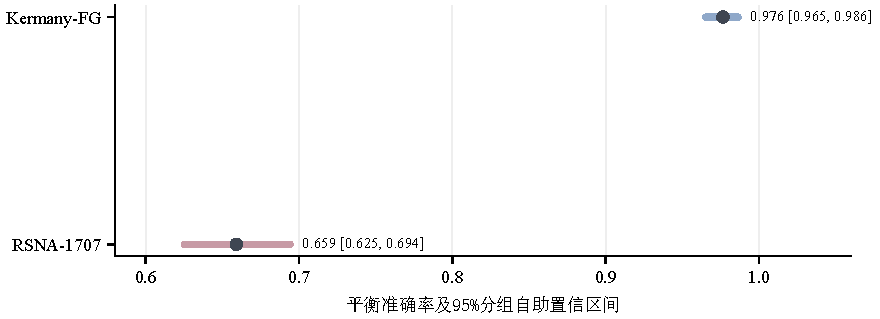
\includegraphics[width=0.80\textwidth]{figures/fig07_bootstrap_ci.pdf}
  \caption{DenseNet121 ERM 三种子集成平衡准确率及 95\% 分组自助置信区间。Kermany-FG 按 624 个文件名派生簇重采样，RSNA-1707 按 442 个 patientId 重采样，共进行 5000 次迭代。}
  \label{fig:bootstrap_ci}
\end{figure}

\textbf{自助法的分组设计依据}：Kermany 测试集按 624 个保守文件名派生簇重采样，RSNA 测试集按 442 个 patientId 重采样。这样做是为了避免把同一分组内可能相关的图像当作完全独立的观察。对于 Kermany，这一分组依据来自文件名规则，并不等同于经过核验的患者标识；相应置信区间应理解为在该保守分组假设下得到的样本不确定性范围。

\textbf{成对比较的统计含义}：在每次自助迭代中使用完全相同的重采样分组来计算 JT 与 ERM 的平衡准确率差值，产生的 5000 个差值构成了配对差值分布。区间不跨越 0，表示在当前测试样本和分组规则下，观察到的差值方向较稳定；这一结果不等同于对其他医院或重新训练结果作总体推断。

\textbf{区间结果与应用意义的区别}。ERM-Reg 相对 ERM 的 RSNA 平衡准确率差值为 +0.0641，成对分组自助法 95\% 区间为 $[+0.0347,+0.0941]$。平衡准确率是两类召回率的平均值，不能换算成“每 100 次判断多正确多少次”。JT 的平衡准确率差值为 +0.1222，但召回率同时下降 0.2115。因而，综合指标的提高不能替代对漏诊和误报代价的具体判断。

\textbf{训练方案成对比较的详细解读}。表~\ref{tab:paired_bootstrap_detail} 以 DenseNet121 JT 相对 ERM 基线在 RSNA-1707 上的成对比较为例，列出了所有八项指标的差值点估计和 95\% 分组自助区间。

\begin{table}[htbp]
\centering
\caption{JT vs ERM 在 RSNA-1707 上的八项指标成对比较（三种子集成，5000 次分组自助法）}
\label{tab:paired_bootstrap_detail}
\renewcommand{\arraystretch}{1.25}
\begin{adjustbox}{max width=\textwidth,center}
\begin{tabular}{lccc}
\toprule
\textbf{指标} & \textbf{ERM 基线} & \textbf{JT} & \textbf{差值 [95\% CI]} \\
\midrule
Accuracy & 0.6674 & 0.7805 & +0.1131 [$+$0.0721, $+$0.1540] \\
Balanced Accuracy & 0.6591 & 0.7813 & +0.1222 [$+$0.0802, $+$0.1638] \\
Precision & 0.6117 & 0.8066 & +0.1949 [$+$0.1313, $+$0.2528] \\
Recall & 0.9648 & 0.7533 & $-$0.2115 [$-$0.2859, $-$0.1371] \\
Specificity & 0.3535 & 0.8093 & +0.4558 [$+$0.3708, $+$0.5351] \\
F1 & 0.7487 & 0.7790 & +0.0303 [$-$0.0026, $+$0.0618] \\
AUROC & 0.8152 & 0.8622 & +0.0470 [$+$0.0221, $+$0.0733] \\
AUPRC & 0.8036 & 0.8689 & +0.0653 [$+$0.0350, $+$0.0977] \\
\bottomrule
\end{tabular}
\end{adjustbox}
\end{table}

八项指标并未沿同一方向变化。特异度增加 0.4558，召回率减少 0.2115；对应的分组自助区间均未跨越 0。在当前测试样本和固定预测下，JT 减少了正常样本误报，同时增加了肺炎样本漏判。AUROC 与 AUPRC 的差值区间也未跨越 0，提示排序性能的变化不只来自阈值移动。F1 差值为 0.0303，区间 $[-0.0026, +0.0618]$ 跨越 0，现有样本不足以排除差值为 0 的可能。这里的区间只反映测试样本重采样的不确定性，不包含重新训练带来的波动，也不能单独建立训练方案与临床收益之间的因果关系。

\textbf{ERM-Reg 和 JT-DBS 的成对比较}。ERM-Reg 相对 ERM 的 RSNA 平衡准确率差值为 +0.0641 [95\% CI: $+$0.0347, $+$0.0941]，区间不包含 0，说明仅靠正则化（颜色扰动 + 标签平滑）就能带来可测的改善。JT-DBS 相对 ERM 的差值为 +0.1131 [$+$0.0700, $+$0.1568]，改善幅度介于 ERM-Reg 和 JT 之间，但 JT-DBS 和 JT 之间的差值很小（$-0.0091$），且该差值的区间包含 0，说明在当前实验设置下，域均衡采样相对于简单联合训练没有带来额外可测的增益。这一结果的一个可能解释是：虽然 Kermany 训练集（约 5,200 张）远大于 RSNA 训练子集（约 1,050 张），但两个来源之间的主要差异可能不在于样本数量，而在于条件分布 $P(Y|X)$ 本身的不同，而域均衡采样只改变边缘分布 $P(\text{source})$，不改条件分布。

\subsection{实验局限性与结果适用范围}

在解读上述实验结果时，需要注意以下几项关键局限性。

\textbf{数据层面的局限}。Kermany 数据集的文件名派生簇只能降低相关样本跨划分的风险，不能等同于经过元数据确认的患者级隔离。因此，Kermany-FG 上的性能指标可能仍包含因同一患者多次检查图像进入不同划分而导致的轻微高估。RSNA-1707 子集（1,707 张）仅占原始 RSNA 完整训练集（26,684 张）的约 6.4\%，是按 patientId 抽取的固定子集而非随机样本，其统计特性可能与完整数据集存在差异。此外，两个数据集在图像格式（JPEG vs DICOM→PNG）、原始分辨率、投照方式（PA vs PA/AP 混合）和患者年龄段（儿科 vs 成人）等方面均存在差异，本研究无法将这些因素的各自贡献分离开来。

\textbf{训练层面的局限}。所有模型仅训练了 4--5 个 epoch，虽然这在迁移学习的常见实践中是合理的（ImageNet 预训练提供了良好的初始化），但不能排除更长时间的训练会改变跨来源泛化表现的结论。学习率、批量大小和权重衰减等超参数均使用常用默认值，未针对跨来源场景进行专门的超参数搜索。

\textbf{评价层面的局限}。RSNA-1707 测试集仅包含 442 张图像（215 NORMAL + 227 PNEUMONIA），样本量有限导致某些指标的置信区间较宽。自助法量化的是固定预测下的测试样本不确定性，不包含重新训练更多随机种子带来的训练不确定性。JT 和 JT-DBS 实验在训练阶段使用了 RSNA 标签，因此其 RSNA 测试集不能被视为严格的外部验证，RSNA 数据的不同部分（按 patientId 划分的 train/val/test）之间的分布相似性可能高于 Kermany 与 RSNA 之间的分布相似性。

\textbf{结论适用范围的限定}。本研究的实验结论，跨来源性能衰减约 30 个百分点、架构选择影响有限、联合训练改善了平衡准确率但以召回率为代价，是在 Kermany 与 RSNA 这两个特定数据集上，使用特定的数据预处理流程（224×224 Resize、ImageNet 归一化）和特定的训练协议（5 epoch、AdamW、迁移学习）下获得的。这些结论不能直接推广到其他胸片数据集、其他医学影像模态或不同的训练配置。特别是，"架构选择对跨来源泛化影响不大"这一结论只在我们测试的三种架构和当前训练设置下成立，不排除在更大规模的数据、更长的训练时间或不同的预训练策略下，架构间的差异会变得显著。

\section{本章小结}

本章先核对数据和实验产物，再报告模型结果。Kermany-FG 通过了文件名派生簇的保守独立性检查，RSNA-1707 通过 patientId 分组和文件完整性检查；NIH 备选子集因患者编号跨划分而未进入严格结果。实验显示，三种 ERM 模型在 Kermany-FG 上的平衡准确率均超过 97\%，在 RSNA-1707 上降至约 66\%。JT 提高了 RSNA 平衡准确率和特异度，却降低了召回率。来源可分性和校准结果说明，跨来源变化还涉及图像统计差异与概率过度自信。第五章将据此回答研究问题，并说明这些结论的适用范围。

% ======================== 第五章 结束语 ========================
\chapter{结束语}

\section{研究结论}

本课程设计以胸片肺炎二分类任务为载体，围绕"单来源训练的高性能模型能不能泛化到不同来源数据"这个核心问题，对 DenseNet121、ConvNeXt-Tiny 和 ViT-B/16 三种深度学习架构进行了跨来源评估。基于 18 次正式训练和全流程可复现实验，我们得到了以下五项主要结论。

\textbf{结论一：单一来源测试集上的高性能不能代表跨来源表现。} 三种架构在 Kermany-FG 上的平衡准确率都超过了 97\%，在 RSNA-1707 上则降到了约 66\%，绝对降幅超过 30 个百分点。DenseNet121 的特异度从 0.9682 降到了 0.3535；在 215 张 RSNA 正常胸片中，模型只正确识别了约 76 张，其余被判成了肺炎。三个随机种子和三种架构都呈现同一方向的下降，说明这不是某一次训练运行的孤立结果。由于两个数据集在人群、标签语义、图像格式和预处理等方面都存在差异，我们将这种性能下降解释为综合性的跨来源分布偏移，而不是归因于某一个单独因素。

\textbf{结论二：在我们的实验设置下，换骨干网络没有带来明显的跨来源优势。} DenseNet121、ConvNeXt-Tiny 和 ViT-B/16 在 RSNA 上的平衡准确率分别为 0.6591、0.6695 和 0.6594，点估计最大相差约 0.01。由于我们没有对架构间差异做专门的成对统计检验，这个结果不宜推广为"不同架构在所有域偏移任务中都等价"。它说明的是：对于我们使用的数据和训练方案，三种架构都受到了明显的跨来源性能下降影响，单纯换网络结构不够。

\textbf{结论三：使用目标来源标注样本的联合训练提高了平衡准确率，但改变了召回率和特异度的取舍。} 将 Kermany 和 RSNA 的训练数据混合后，DenseNet121 在 RSNA 上的平衡准确率从 0.6591 提高到 0.7813，特异度从 0.3535 提高到 0.8093，但召回率从 0.9648 降到了 0.7533。换句话说，正常图像的误报减少了，但肺炎图像的漏判增加了。对于筛查任务，这种变化不能只用一个综合指标来评价，还需要结合具体应用场景对漏诊和误报的代价进行权衡。本课程设计属于回顾性数据实验，不对该工作点的临床可接受性做判断。

\textbf{结论四：两个来源在所测图像统计上具有较强的可分性，但具体成因还需要进一步分析。} 标签匹配条件下的来源分类 AUROC 为 0.9441，而且分类器没有使用宽高比特征。这表明两个来源在亮度、对比度、区域统计和熵等测量值上存在差异，但不能据此确定设备、人群或预处理中的哪一项是主要原因。Kermany 和 RSNA 的平均宽高比分别约为 1.45 和 1.00，反映出预处理方式并不一致；不过我们没有做保持比例与拉伸缩放的对照实验，因此不能量化宽高比或某个预处理步骤对分类性能的独立贡献。

\textbf{结论五：实验记录决定了结果能否被核查。} 本次课程设计用脚本组织 18 次训练，以 51 项测试检查核心模块，并通过冻结清单、文件哈希和自动验收核对数据身份与实验产物。这些记录不能消除实验误差，但有助于区分模型表现变化与数据版本、随机种子或评价协议不一致造成的差异。\vspace{0.5cm}

\textbf{总结}：在当前数据和训练协议下，单来源训练模型从 Kermany 转到 RSNA 后出现约 30 个百分点的平衡准确率下降；三种骨干网络均受到影响；使用 RSNA 标注训练样本的联合训练提高了平衡准确率和特异度，同时降低了召回率。这些结果适用于本研究的数据划分和评价设置，不代表其他医院或其他胸片任务会出现相同幅度的变化。

\section{对模式识别学科的认识与体会}

这次课程设计使我们对模式识别中的几个基本问题有了更具体的认识。

同分布测试只是实验设定，不能代替新来源验证。项目早期主要关注 Kermany-FG；加入 RSNA-1707 后，三种模型的平衡准确率都下降了约 30 个百分点。错误结构也随之改变：模型仍识别出多数肺炎图像，却把大量正常图像判为肺炎。这段经历使我们在比较指标前先核对测试数据代表的人群、标签和采集条件。

单一指标还会掩盖错误结构。DenseNet121 在 RSNA-1707 上保持了 0.9648 的召回率，但特异度只有 0.3535。JT 将平衡准确率提高到 0.7813，同时把召回率降到 0.7533。若只看平衡准确率，容易忽略漏判增加；若只看召回率，又会忽略正常图像的大量误报。混淆矩阵、召回率、特异度和校准指标共同描述了模型在哪类样本上失败。

数据划分也是本项目中最容易被低估的环节。Kermany 缺少可核验的患者映射，我们只能依据文件名构造保守簇，降低相关图像跨划分的风险。RSNA 具有 patientId，可以按患者进行分组。两种数据条件不同，报告时也必须使用不同的证据强度。这个过程让我们认识到，数据标识和划分规则并非训练前的例行准备，它们决定了测试结果能否被合理解释。

自动化在本项目中的作用主要是减少遗漏。18 次训练涉及多个模型、随机种子和测试集，如果依靠手工命名和逐项核对，很容易混淆结果。配置文件、逐图预测和验收脚本让实验步骤可以重复执行，也便于在数字出现异常时回查来源。对课程设计而言，这些工具服务于实验本身，不构成独立的研究贡献；它们的实际作用是让结果更容易核对。

如果重新开展一次实验，我们会在设计阶段更早确定患者或样本分组规则，并加入保持宽高比的预处理对照。我们也会把外部测试集的标签语义差异写入实验方案，而不是等结果下降后再解释。相比继续增加模型数量，这些调整更有助于判断跨来源性能变化究竟来自数据、标签还是预处理。

\section{每人工作划分}

本课程设计由五名组员协作完成，工作划分表如下。

\begin{table}[htbp]
\centering
\caption{组员工作划分}
\label{tab:workload}
\renewcommand{\arraystretch}{1.8}
\begin{adjustbox}{max width=\textwidth,center}
\begin{tabular}{cccp{7.2cm}}
\toprule
\textbf{姓名} & \textbf{学号} & \textbf{占比} & \textbf{主要工作内容} \\
\midrule
\rule{0pt}{1.2cm} & & & \\
\midrule
\rule{0pt}{1.2cm} & & & \\
\midrule
\rule{0pt}{1.2cm} & & & \\
\midrule
\rule{0pt}{1.2cm} & & & \\
\midrule
\rule{0pt}{1.2cm} & & & \\
\bottomrule
\end{tabular}
\end{adjustbox}
\end{table}

\section{未来工作展望}

后续工作应优先补足当前结论中无法区分的因素，而非继续堆叠模型。

\textbf{（一）纳入更多样化的数据来源并对比更多域泛化算法。} 目前仅使用了两个胸片数据集，无法将域偏移的来源拆解到单个因素（设备、人群、标注）。后续可纳入来自更多国家和设备厂商的数据集，构建多维度可控的跨来源评估基准。同时，当前仅评估了基于数据和采样层面的训练方案，未涉及算法层面的域泛化方法（如 CORAL、DANN、IRM），这些方法可在现有实验基础设施上作为插件接入并对比。

\textbf{（二）检验胸片自监督预训练与多标签任务。} 当前实验没有比较 ImageNet 预训练和胸片自监督预训练。后续可在相同数据划分和训练预算下比较 MAE、DINO 等初始化方式，观察跨来源指标是否改变。多标签扩展则需要先统一不同数据集的标签定义，再考察胸腔积液、气胸和结节等类别是否呈现相同的性能衰减。

\textbf{（三）前瞻性临床验证与模型公平性评估。} 当前实验全部为回顾性研究，模型在真实临床工作流中的表现（作为"第二阅片者"辅助或分诊工具）尚需前瞻性验证。同时，跨来源性能在不同人口统计学子群（年龄组、性别）上的差异值得进行公平性审计，确保模型部署不会对某些患者群体造成不成比例的伤害。

\textbf{（四）在其他影像任务上复核评估流程。} 数据审计、固定划分、逐图预测和分组统计可以用于皮肤镜、眼底或病理图像研究，但患者标识、标签语义和采集流程需要按任务重新定义。只有完成相应复核后，才能判断本研究的评估流程是否适用，不能由胸片实验直接推定其通用性。

% ======================== 附录 ========================
\appendix

\chapter{主要模块代码}

本附录列出系统的四个核心模块完整代码。按照课程设计要求，代码中的注释量不低于代码量的 1:1。每个模块的代码前附有功能概述和设计说明。

\section{数据集加载与验证模块 (data.py)}

\textbf{功能概述}：本模块是系统数据层的核心组件，负责图像文件枚举、ImageFolder 格式目录验证、样本列表构建、分层划分和 PyTorch Dataset 封装。所有公开函数均采用确定性实现（字典序排序、显式随机种子），确保相同输入在任何操作系统上产生相同输出。

\begin{lstlisting}[language=Python, caption={数据集加载与验证模块（data.py）}, label={lst:data}]
"""
数据集工具模块 —— 胸片肺炎分类项目的数据层核心。

设计原则：
  1. 确定性优先：所有遍历和排序操作使用字典序，消除操作系统文件系统差异。
     这是因为不同操作系统的文件系统（ext4/NTFS/APFS）对 inode 顺序的处理不同，
     如果不强制字典序排序，同一目录下的文件列表顺序在不同机器上可能不一致，
     进而导致 DataLoader 分发批次序列不同，即使固定随机种子也无法保证可复现。
  2. 显式验证：DatasetValidationResult 提供结构化的验证输出，而非抛出异常即止。
     这样上层调用者可以根据验证结果决定是否继续执行，而不是被异常强制中断。
  3. 接口统一：XRayImageDataset 和 XRaySampleDataset 遵循相同的 torch Dataset 接口，
     确保训练和评价管线可以无差别地使用两种数据来源。
  4. 类别权重计算：使用逆频率加权，确保分类器不会被多数类样本主导。
     在 Kermany 数据集中 PNEUMONIA 约为 NORMAL 的 2.7 倍，如果不加权，
     模型可能学到"始终预测 PNEUMONIA"的捷径即可获得较低的损失。
"""

from __future__ import annotations

import json
import random
from dataclasses import dataclass, field
from pathlib import Path
from typing import Any, Callable, Iterable, Mapping, Sequence

# ---------------------------------------------------------------------------
# 全局常量 —— 定义本模块和数据管线的标准约定
# ---------------------------------------------------------------------------
# 二分类任务的类别名称，按字母序排列以保证确定性（NORMAL 在 PNEUMONIA 之前）
DEFAULT_CLASSES = ("NORMAL", "PNEUMONIA")
# 数据集的标准三个划分名称。train 用于模型参数更新，val 用于检查点选择与超参调优，
# test 仅用于最终评估，不应在训练过程中被访问。
DEFAULT_SPLITS = ("train", "val", "test")
# 支持的图像文件扩展名。全部转为小写比较，实现大小写不敏感匹配。
# 包含 BMP 和 TIFF 是为了兼容可能的原始医学影像格式，尽管本实验主要使用 JPEG 和 PNG。
IMAGE_EXTENSIONS = (".jpg", ".jpeg", ".png", ".bmp", ".tif", ".tiff")


def _as_tuple(values: Iterable[str]) -> tuple[str, ...]:
    """将任意可迭代的字符串序列转换为不可变元组，用于数据类字段。

    使用元组而非列表的原因：dataclass 的 frozen 模式下，可变字段（如 list）
    实际上仍然可以被修改（Python 不阻止修改 list 的元素）。转为 tuple 后真正不可变。
    """
    return tuple(str(value) for value in values)


def _relative(path: Path, root: Path) -> str:
    """
    计算文件路径相对于根目录的 POSIX 风格相对路径。

    如果路径不在根目录下（例如符号链接指向外部），则返回绝对路径的
    POSIX 表示。此函数专门用于验证报告中路径的可移植显示——
    Windows 风格的反斜杠路径在 JSON 中需要额外转义，POSIX 风格更干净。

    注意：使用 as_posix() 而非 str(path)，前者在所有平台上都产生正斜杠。
    """
    try:
        return path.relative_to(root).as_posix()
    except ValueError:
        # 符号链接指向外部目录时 relative_to 会抛出 ValueError，
        # 此时回退到绝对路径的 POSIX 表示
        return path.as_posix()


def list_image_files(
    directory: Path | str,
    extensions: Sequence[str] = IMAGE_EXTENSIONS,
) -> list[Path]:
    """
    以确定性顺序递归枚举目录下的所有图像文件。

    确定性由两个操作保证：
      (a) 扩展名集合先转为小写再匹配，实现大小写不敏感。
          例如 .JPG 和 .jpg 都会被识别为图像文件。
      (b) 结果列表按完整路径字符串进行字典序排序。
          因此，在相同的目录内容下，无论在何种操作系统上运行，返回的列表顺序完全一致。

    选择 rglob 而非 iterdir 递归的原因：原始 Kermany 数据集可能存在嵌套子目录
    （如 train/NORMAL/ 下还有子文件夹），rglob 能覆盖所有层级。

    参数：
      directory: 要扫描的根目录路径。如果目录不存在，返回空列表而非抛出异常，
                 因为在验证上下文中"目录不存在"是一个需要报告的状态，不应导致程序崩溃。
      extensions: 视为图像文件的扩展名列表，默认使用 IMAGE_EXTENSIONS。
    返回：
      排序后的 Path 对象列表。
    """
    directory = Path(directory)
    if not directory.exists():
        return []

    suffixes = {ext.lower() for ext in extensions}
    return sorted(
        path
        for path in directory.rglob("*")
        if path.is_file() and path.suffix.lower() in suffixes
    )


@dataclass
class DatasetValidationResult:
    """
    ImageFolder 格式数据集的结构化验证结果。

    此类使用 Python dataclass 而非普通字典的设计理由：
      (a) 字段类型明确，IDE 可提供自动补全，减少拼写错误；
      (b) to_dict() / to_json() 提供标准化的序列化接口，确保 JSON 输出的键名一致；
      (c) ok 属性提供单一真值来源（single source of truth），避免调用方自行组合
          多个条件判断时遗漏某个检查项。

    字段说明：
      root: 被验证的数据集根目录。
      classes: 期望的类别名称元组（如 ("NORMAL", "PNEUMONIA")）。
      splits: 期望的划分名称元组（如 ("train", "val", "test")）。
      counts: 三层嵌套字典 counts[split][class_name] = 图像数量。
              嵌套结构而非扁平结构的原因是：调用方通常需要按划分查看类别分布。
      missing_dirs: 不存在的期望目录列表。这是最严重的验证问题，意味着数据不完整。
      empty_dirs: 存在但为空的类别目录列表。空目录可能是数据准备脚本的 bug。
      unexpected_class_dirs: 出现非期望类别名的目录。可能是遗留的临时目录或数据污染。
      invalid_images: 无法被 Pillow 打开的损坏图像列表。每项包含 path 和 error 两个字段。
      image_extensions: 验证时使用的扩展名集合，记录此信息以便审计时确认使用的扩展名。
    """

    root: Path
    classes: tuple[str, ...]
    splits: tuple[str, ...]
    counts: dict[str, dict[str, int]]
    missing_dirs: list[str] = field(default_factory=list)
    empty_dirs: list[str] = field(default_factory=list)
    unexpected_class_dirs: dict[str, list[str]] = field(default_factory=dict)
    invalid_images: list[dict[str, str]] = field(default_factory=list)
    image_extensions: tuple[str, ...] = IMAGE_EXTENSIONS

    @property
    def total_images(self) -> int:
        """返回所有划分中所有类别的图像总数。

        计算方式是两次求和：先对每个划分内的所有类别求和（内层 sum），
        再对所有划分求和（外层 sum）。这比维护一个单独的 total 字段更安全，
        因为 total 可能与 counts 的实际值不同步。
        """
        return sum(sum(class_counts.values()) for class_counts in self.counts.values())

    @property
    def ok(self) -> bool:
        """
        数据集的整体健康状态。

        只有当以下四项全部为空时才是 OK：
          - 没有缺失目录（数据完整）
          - 没有空目录（数据非空）
          - 没有意外的类别目录（目录结构规范）
          - 没有损坏的图像（图像文件可读）

        使用 not any([...]) 的短路求值：一旦发现任何一个列表非空，立即返回 False。
        """
        return not (
            self.missing_dirs
            or self.empty_dirs
            or self.unexpected_class_dirs
            or self.invalid_images
        )

    def to_dict(self) -> dict[str, object]:
        """将验证结果序列化为 JSON 兼容的字典。

        将 Path 对象转为 POSIX 字符串，将元组转为列表（JSON 不支持元组类型），
        以便 json.dumps 直接序列化。
        """
        return {
            "root": self.root.as_posix(),
            "classes": list(self.classes),
            "splits": list(self.splits),
            "counts": self.counts,
            "total_images": self.total_images,
            "missing_dirs": self.missing_dirs,
            "empty_dirs": self.empty_dirs,
            "unexpected_class_dirs": self.unexpected_class_dirs,
            "invalid_images": self.invalid_images,
            "image_extensions": list(self.image_extensions),
            "ok": self.ok,
        }

    def to_json(self, indent: int = 2) -> str:
        """将验证结果直接序列化为 JSON 字符串。

        ensure_ascii=False 保留中文字符不转义，indent=2 使输出人类可读。
        """
        return json.dumps(self.to_dict(), ensure_ascii=False, indent=indent)


def validate_dataset_layout(
    data_root: Path | str,
    class_names: Sequence[str] = DEFAULT_CLASSES,
    splits: Sequence[str] = DEFAULT_SPLITS,
    extensions: Sequence[str] = IMAGE_EXTENSIONS,
    verify_images: bool = False,
    require_non_empty: bool = True,
) -> DatasetValidationResult:
    """
    验证 ImageFolder 格式数据集的目录结构和图像完整性。

    这是整个数据处理管线的入口守卫——所有训练和评价脚本在启动前
    必须通过此函数的验证。验证逻辑按以下顺序执行：
      1. 检查根目录是否存在。这是最快失败的检查，避免后续无意义的目录遍历。
      2. 对每个划分 (train/val/test) 和每个类别 (NORMAL/PNEUMONIA)，
         检查对应的子目录是否存在。
      3. 枚举每个子目录中的图像文件，记录数量。
      4. 可选：使用 Pillow 的 Image.verify() 逐张核验图像可读性。
         verify() 仅检查文件头完整性（不解码全部像素），比完整加载快得多。
      5. 可选：检查是否存在非预期的类别目录名（如遗留的临时目录）。

    参数：
      data_root: 数据集根目录路径。
      class_names: 期望的类别名称序列。
      splits: 期望的划分名称序列。如果数据只有 train/test 两个划分，
              传入 ("train", "test") 即可。
      extensions: 视为图像文件的扩展名集合。
      verify_images: 是否逐张核验图像可读性。默认为 False 以加快常规验证速度。
      require_non_empty: 发现空类别目录时是否标记为问题。默认为 True。
    返回：
      DatasetValidationResult 实例，其中 ok 属性为 True 表示通过全部检查。
    """
    root = Path(data_root)
    classes = _as_tuple(class_names)
    split_names = _as_tuple(splits)
    ext_names = _as_tuple(extensions)

    # 初始化三层嵌套计数字典：counts[split][class_name] = 0
    # 预初始化为 0 的好处：即使某个目录不存在，JSON 报告中也会显示该目录的计数为 0
    # 而非缺失该键，便于下游脚本统一解析
    counts: dict[str, dict[str, int]] = {
        split: {class_name: 0 for class_name in classes} for split in split_names
    }
    missing_dirs: list[str] = []
    empty_dirs: list[str] = []
    unexpected_class_dirs: dict[str, list[str]] = {}
    invalid_images: list[dict[str, str]] = []

    # 根目录不存在是第一个检查点——后续所有操作都依赖根目录存在
    if not root.exists():
        missing_dirs.append(root.as_posix())
        return DatasetValidationResult(
            root=root, classes=classes, splits=split_names,
            counts=counts, missing_dirs=missing_dirs,
            empty_dirs=empty_dirs, unexpected_class_dirs=unexpected_class_dirs,
            invalid_images=invalid_images, image_extensions=ext_names,
        )

    # 仅在调用方明确要求时才启用图像验证。
    # Image.verify() 虽然比完整解码快，但对于 5000+ 张图像的数据集仍然需要数秒。
    # 因此默认为 False，在需要彻底检查时（如首次下载数据后）手动开启。
    verifier = _verify_image if verify_images else None

    for split in split_names:
        split_dir = root / split
        if not split_dir.is_dir():
            missing_dirs.append(_relative(split_dir, root))
            # 注意：目录不存在时 continue 而非 return，因为其他划分可能正常。
            # 我们希望一次性报告所有问题，而不是修一个报一个。
            continue

        # 检查是否有不在期望类别列表中的子目录（如遗留的临时目录、隐藏文件夹）
        # 这些意外目录不会导致验证失败（ok 仍为 True），但会在报告中列出以引起注意
        unexpected = sorted(
            path.name
            for path in split_dir.iterdir()
            if path.is_dir() and path.name not in classes
        )
        if unexpected:
            unexpected_class_dirs[split] = unexpected

        for class_name in classes:
            class_dir = split_dir / class_name
            if not class_dir.is_dir():
                missing_dirs.append(_relative(class_dir, root))
                continue

            files = list_image_files(class_dir, ext_names)
            counts[split][class_name] = len(files)
            if require_non_empty and not files:
                empty_dirs.append(_relative(class_dir, root))

            if verifier is not None:
                invalid_images.extend(
                    {"path": _relative(path, root), "error": error}
                    for path, error in verifier(files)
                )

    return DatasetValidationResult(
        root=root, classes=classes, splits=split_names,
        counts=counts, missing_dirs=missing_dirs,
        empty_dirs=empty_dirs, unexpected_class_dirs=unexpected_class_dirs,
        invalid_images=invalid_images, image_extensions=ext_names,
    )


def _verify_image(files: Sequence[Path]) -> list[tuple[Path, str]]:
    """
    使用 Pillow 的 Image.verify() 逐张核验图像文件的可读性。

    verify() 方法仅检查文件头部的完整性（不解码全部像素数据），
    因此比完整的 Image.open().load() 快得多。它足以检测：
      - 文件截断（下载不完整）
      - 文件头损坏（存储介质错误）
      - 格式不匹配（扩展名与实际内容不符）

    但不检测像素数据的完整性（如 JPEG 的 DCT 系数错误）。
    对于大规模数据集的快速筛查，这个精度已经足够。
    """
    try:
        from PIL import Image
    except ImportError as exc:
        raise RuntimeError("Pillow is required when verify_images=True") from exc

    invalid: list[tuple[Path, str]] = []
    for path in files:
        try:
            with Image.open(path) as image:
                image.verify()
        except Exception as exc:
            # 捕获所有异常类型，因为 Pillow 对不同格式的损坏文件可能抛出
            # 不同的异常类型（UnidentifiedImageError, OSError 等）
            invalid.append((path, str(exc)))
    return invalid


def build_samples(
    data_root: Path | str,
    split: str,
    class_names: Sequence[str] = DEFAULT_CLASSES,
    extensions: Sequence[str] = IMAGE_EXTENSIONS,
) -> list[tuple[Path, int]]:
    """
    为给定的划分构建 (图像路径, 类别索引) 样本列表。

    样本按图像路径的 POSIX 字符串进行字典序排序，保证确定性。
    类别索引由 class_names 中的位置决定（0 = NORMAL, 1 = PNEUMONIA）。

    排序的重要性：PyTorch 的 DataLoader 在多 worker 模式下的数据分发顺序
    取决于 Dataset 返回样本的顺序。如果这个顺序在不同运行中不同（例如受
    文件系统 inode 顺序影响），即使固定了所有随机种子，模型接收到的批次
    序列仍然可能不同，进而导致训练结果出现微小的不可复现差异。

    此函数是 XRayImageDataset 的底层实现，被训练和评价管线共同调用。
    """
    root = Path(data_root)
    samples: list[tuple[Path, int]] = []
    for class_index, class_name in enumerate(class_names):
        class_dir = root / split / class_name
        for path in list_image_files(class_dir, extensions):
            samples.append((path, class_index))
    # 按路径的 POSIX 字符串排序，确保跨平台确定性
    return sorted(samples, key=lambda item: item[0].as_posix())


def stratified_holdout_indices(
    samples: Sequence[tuple[Path, int]],
    holdout_fraction: float,
    seed: int = 42,
) -> tuple[list[int], list[int]]:
    """
    按类别分层的留出法索引划分。

    对每个类别独立地进行随机打乱和划分，确保 holdout 集合中
    各类别的比例与原始训练集一致。这是分层抽样（stratified sampling）的
    标准实现——不对全部样本一次性 shuffle，而是逐类 shuffle 后切分。

    为什么需要分层：如果直接随机划分，可能某一类在 holdout 中的比例
    与原始训练集显著不同（特别是小样本类别），导致 holdout 验证集
    不能准确反映训练集的类别分布。逐类分层可以避免这个问题。

    参数：
      samples: 由 build_samples 返回的完整样本列表。
      holdout_fraction: 留出比例（例如 0.2 表示留出 20%）。
      seed: 随机种子，保证可复现的分层抽样。
    返回：
      (train_indices, holdout_indices) 两个排序后的索引列表。
      排序是为了确定性——调用方可以根据排序后的索引使用 Subset 或直接切片。
    """
    if holdout_fraction <= 0 or holdout_fraction >= 1:
        raise ValueError("holdout_fraction must be in the interval (0, 1)")

    # 按类别标签分组索引。
    # setdefault 比先检查 key 是否存在再初始化更简洁，避免了 KeyError 的 try/except。
    by_label: dict[int, list[int]] = {}
    for index, (_, label) in enumerate(samples):
        by_label.setdefault(int(label), []).append(index)

    rng = random.Random(seed)
    train_indices: list[int] = []
    holdout_indices: list[int] = []
    for label_indices in by_label.values():
        shuffled = list(label_indices)
        rng.shuffle(shuffled)
        # 确保每类至少保留 1 个训练样本和 1 个 holdout 样本。
        # 这是为了防止极端情况——如果某个类只有 2 张图像，不做此保护
        # 可能导致 train 或 holdout 中完全没有该类的样本。
        holdout_count = max(1, round(len(shuffled) * holdout_fraction))
        holdout_count = min(holdout_count, len(shuffled) - 1)
        holdout_indices.extend(shuffled[:holdout_count])
        train_indices.extend(shuffled[holdout_count:])

    # 排序是为了确定性：即使 shuffle 结果相同，extend 的顺序可能因
    # by_label 的键迭代顺序不同而变化（Python 3.7+ 保证 dict 插入顺序，
    # 但为了向前兼容和代码清晰，仍显式排序）
    return sorted(train_indices), sorted(holdout_indices)


# 安全导入 PyTorch：如果 torch 不可用，Dataset 基类退化为普通 object。
# 这允许本模块在不安装 PyTorch 的环境中仍能执行数据验证功能
# （如 check_dataset.py 在 CI 中运行时不依赖 GPU 和 PyTorch）。
try:
    from torch.utils.data import Dataset as _TorchDataset
except Exception:
    _TorchDataset = object  # type: ignore[misc,assignment]


class XRayImageDataset(_TorchDataset):
    """
    标准 ImageFolder 格式的 PyTorch Dataset 封装。

    构造函数按字典序遍历给定划分和类别的目录，构建确定性排序的
    样本列表。支持通过 torchvision transform 进行在线数据增强和归一化。

    关键设计决策：
      - 样本列表在 __init__ 中一次性构建完成，后续 __getitem__ 仅做索引查找。
        这避免了在每个 epoch 开始前重新扫描文件系统。
      - 图像在 __getitem__ 中即时加载（而非预加载），避免 5000+ 张图像
        同时驻留内存导致 OOM。对于 SSD 上的数据，即时加载的 I/O 开销可忽略。

    使用示例：
      dataset = XRayImageDataset("data/processed/kermany_grouped_seed42",
                                  split="train",
                                  transform=train_transform)
      loader = DataLoader(dataset, batch_size=32, shuffle=True)
    """

    def __init__(
        self,
        data_root: Path | str,
        split: str,
        class_names: Sequence[str] = DEFAULT_CLASSES,
        transform: Callable | None = None,
        extensions: Sequence[str] = IMAGE_EXTENSIONS,
    ) -> None:
        self.data_root = Path(data_root)
        self.split = split
        self.class_names = _as_tuple(class_names)
        # 建立类别名称到索引的映射字典，供调试和日志使用。
        # 例如：self.class_to_idx["PNEUMONIA"] 返回 1
        self.class_to_idx = {
            class_name: class_index
            for class_index, class_name in enumerate(self.class_names)
        }
        self.transform = transform
        # 在构造函数中即完成全部文件的扫描和排序。
        # 如果数据目录不存在或为空，samples 将为空列表，
        # 后续 DataLoader 会立即发现（len=0）而非在训练中途崩溃。
        self.samples = build_samples(
            self.data_root, split, self.class_names, extensions,
        )

    def __len__(self) -> int:
        """返回数据集中的图像总数。DataLoader 使用此值确定每个 epoch 的迭代次数。"""
        return len(self.samples)

    def __getitem__(self, index: int):
        """
        返回第 index 个样本的 (变换后图像张量, 类别标签) 对。

        Pillow Image.open() 在每次 __getitem__ 调用时执行（而非预加载），
        避免将全部图像一次性加载到内存中。对于 224×224 的 JPEG 图像，
        单张解码约需 1-2ms，在 batch_size=32 时 I/O 开销约 30-60ms，
        相对于 GPU 前向传播的 50-100ms 来说可以接受。

        注意：这里使用 image.convert("RGB") 而非直接使用打开的图像。
        原因是某些医学影像可能以灰度（L 模式）或 RGBA 模式存储，
        而预训练模型期望 3 通道 RGB 输入。convert("RGB") 统一处理所有情况：
        L→RGB 复制灰度到三通道，RGBA→RGB 丢弃 alpha 通道。
        """
        try:
            from PIL import Image
        except ImportError as exc:
            raise RuntimeError("Pillow is required to load dataset images") from exc

        path, label = self.samples[index]
        with Image.open(path) as image:
            loaded_image: Any = image.convert("RGB")
            if self.transform is not None:
                loaded_image = self.transform(loaded_image)
        return loaded_image, label


class XRaySampleDataset(_TorchDataset):
    """
    基于显式样本列表的 PyTorch Dataset 封装。

    与 XRayImageDataset 的区别在于：样本列表不通过扫描目录获得，
    而是由调用方在构造时显式传入。这使得本类适用于以下场景：
      - RSNA 按 patientId 自定义划分（而非 ImageFolder 的固定目录结构）
      - Kermany + RSNA 混合训练（样本来自多个根目录，物理上分散在不同文件夹）
      - 从训练集中留出的 holdout 验证子集（Subset 的替代方案，
        Subset 要求底层 Dataset 不变，而 XRaySampleDataset 可以独立定义）

    设计权衡：XRaySampleDataset 的灵活性以调用方的责任为代价——
    调用方必须确保传入的样本列表中的路径是有效的、标签是正确的，
    Dataset 本身不做目录扫描和验证。
    """

    def __init__(
        self,
        data_root: Path | str,
        samples: Sequence[tuple[Path | str, int]],
        split: str = "manifest",
        class_names: Sequence[str] = DEFAULT_CLASSES,
        transform: Callable | None = None,
    ) -> None:
        self.data_root = Path(data_root)
        self.split = split
        self.class_names = _as_tuple(class_names)
        self.class_to_idx = {
            class_name: class_index
            for class_index, class_name in enumerate(self.class_names)
        }
        self.transform = transform
        # 规范化：统一将所有路径转为 Path 对象。
        # 如果是相对路径（字符串），自动拼接 data_root 前缀转为绝对路径。
        # 绝对路径允许 DataLoader 的 num_workers > 0 时子进程正确找到文件，
        # 因为子进程的当前工作目录可能与主进程不同。
        self.samples = [
            (path if isinstance(path, Path) else self.data_root / str(path), int(label))
            for path, label in samples
        ]

    def __len__(self) -> int:
        return len(self.samples)

    def __getitem__(self, index: int):
        try:
            from PIL import Image
        except ImportError as exc:
            raise RuntimeError("Pillow is required to load dataset images") from exc

        path, label = self.samples[index]
        with Image.open(path) as image:
            loaded_image: Any = image.convert("RGB")
            if self.transform is not None:
                loaded_image = self.transform(loaded_image)
        return loaded_image, label


def build_class_weights(
    counts: Mapping[str, int],
    class_names: Sequence[str] = DEFAULT_CLASSES,
) -> list[float]:
    """
    计算逆频率类别权重，用于加权交叉熵损失函数。

    权重公式：w_c = total / (K * n_c)
    其中 total 为全部样本数，K 为类别数，n_c 为类别 c 的样本数。

    这一公式确保：
      - 样本数少的类别获得 w_c > 1 的权重（被模型更"重视"）
      - 样本数多的类别获得 w_c < 1 的权重（被模型更"忽视"）
      - 所有权重的均值为 1.0（权重之和为 K）

    以 Kermany-FG 训练集为例：NORMAL 约 1113 张，PNEUMONIA 约 2994 张。
    w_normal = 4107/(2*1113) ~= 1.845, w_pneumonia = 4107/(2*2994) ~= 0.686。
    少数类（NORMAL）获得更高权重，多数类（PNEUMONIA）获得更低权重。

    注意：如果某个类别样本数为 0，则返回全 1 权重（等价于不加权）。
    这种情况可能发生在数据准备阶段出错时，全 1 权重至少允许训练继续
    而非抛出除零异常，但结果将不可靠——调用方应检查日志中的警告。
    """
    values = [int(counts.get(class_name, 0)) for class_name in class_names]
    total = sum(values)
    if total <= 0 or any(value <= 0 for value in values):
        return [1.0 for _ in class_names]
    num_classes = len(values)
    return [total / (num_classes * value) for value in values]


def format_validation_report(result: DatasetValidationResult) -> str:
    """
    将 DatasetValidationResult 格式化为紧凑的人类可读报告。

    报告包括：
      1. 根目录路径和整体健康状态（OK / INVALID）
      2. 按划分 × 类别交叉的样本计数表（对齐的文本表格）
      3. 缺失目录、空目录、意外目录和损坏图像的逐项列表

    损坏图像最多列出前 20 个（避免超长输出掩盖其他重要信息），
    超出部分显示省略信息（如"还有 15 张损坏图像未列出"）。
    """
    lines = [
        f"Dataset root: {result.root.as_posix()}",
        f"Status: {'OK' if result.ok else 'INVALID'}",
        f"Total images: {result.total_images}",
        "",
        "Counts:",
    ]

    # 构建对齐的计数表格。动态计算列宽：每列宽度取表头长度和所有行内容
    # 长度的最大值，确保所有列都对齐。
    header = ["split", *result.classes, "total"]
    widths = [max(len(item), 5) for item in header]
    rows: list[list[str]] = []
    for split in result.splits:
        class_counts = result.counts[split]
        row = [
            split,
            *(str(class_counts[class_name]) for class_name in result.classes),
            str(sum(class_counts.values())),
        ]
        rows.append(row)
        widths = [max(width, len(value)) for width, value in zip(widths, row)]

    lines.append("  " + "  ".join(value.ljust(width) for value, width in zip(header, widths)))
    for row in rows:
        lines.append("  " + "  ".join(value.ljust(width) for value, width in zip(row, widths)))

    # 逐项列出验证问题，每个问题一行，方便 grep 和日志分析
    if result.missing_dirs:
        lines.extend(["", "Missing directories:"])
        lines.extend(f"  - {path}" for path in result.missing_dirs)
    if result.empty_dirs:
        lines.extend(["", "Empty class directories:"])
        lines.extend(f"  - {path}" for path in result.empty_dirs)
    if result.unexpected_class_dirs:
        lines.extend(["", "Unexpected class directories:"])
        for split, directories in sorted(result.unexpected_class_dirs.items()):
            lines.append(f"  - {split}: {', '.join(directories)}")
    if result.invalid_images:
        lines.extend(["", "Invalid images:"])
        for item in result.invalid_images[:20]:
            lines.append(f"  - {item['path']}: {item['error']}")
        if len(result.invalid_images) > 20:
            lines.append(f"  - ... {len(result.invalid_images) - 20} more")

    return "\n".join(lines)
\end{lstlisting}

\section{概率校准模块 (calibration.py)}

\textbf{功能概述}：本模块实现了基于 Temperature Scaling 的概率校准算法，包括预测文件加载与校验、温度参数的网格搜索优化、校准后概率计算以及 ECE / MCE / Brier Score / NLL 等五项校准指标的评估。所有计算均为纯 Python/NumPy 实现，不依赖 PyTorch，使得校准分析可以在不安装 GPU 环境的机器上高效执行。

\begin{lstlisting}[language=Python, caption={概率校准模块（calibration.py）}, label={lst:calibration}]
"""
概率校准模块 —— Temperature Scaling 的完整实现。

校准问题的背景：
  现代深度神经网络虽然分类准确率高，但 Softmax 输出的"概率"通常
  过度自信（overconfident）——模型声称 99% 置信度的预测中，实际
  正确率可能远低于 99%。在医学影像场景中，这种校准不良会导致医生
  对模型的错误预测产生不恰当的信任，可能造成漏诊或误诊。

Temperature Scaling 的原理：
  在验证集上学习一个标量温度参数 T > 0，将原始 logits 除以 T 后
  再输入 Softmax。T > 1 使概率分布更"平滑"（降低过度自信），
  T < 1 使概率分布更"尖锐"。T 的最优值通过最小化验证集的负对数
  似然（Negative Log-Likelihood, NLL）在网格搜索中确定。

关键性质：温度缩放不改变模型的排序——argmax 预测在任意 T > 0 下
保持不变。这确保了校准不会改变分类决策本身，只改变概率的数值质量。

实现选择：本模块使用纯 Python/NumPy 实现而非 PyTorch 实现的原因是：
  1. 校准分析只需要操作已有的预测 CSV 文件，不需要重新加载模型权重；
  2. 避免引入 PyTorch 的 GPU 依赖，使得校准可以在任何环境（包括 CI）中运行；
  3. 1,951 个候选温度的网格搜索在 NumPy 中约 0.5 秒即可完成，
     不需要 GPU 加速。
"""

from __future__ import annotations

import csv
import math
from dataclasses import asdict, dataclass
from pathlib import Path
from typing import Sequence


@dataclass(frozen=True)
class CalibratedPrediction:
    """
    单张图像的经过验证的预测记录。

    使用 frozen=True 确保记录在创建后不可修改，防止在校准分析
    过程中意外改动原始预测数据。这是防御性编程——校准分析涉及
    多次遍历预测列表（NLL 计算、分桶、ECE 计算），不可变性
    保证每次遍历看到的数据完全一致。

    字段说明：
      path: 图像文件的相对路径，用于追踪错误样本。
      true_label: 真实标签（"NORMAL" 或 "PNEUMONIA"）。
      predicted_label: 模型在阈值 0.5 下的预测标签。
      score: PNEUMONIA 类别的 Softmax 概率（即阳性概率）。
    """
    path: str
    true_label: str
    predicted_label: str
    score: float


@dataclass(frozen=True)
class CalibrationBin:
    """
    可靠性图中的一个等宽置信度桶。

    可靠性图（Reliability Diagram）将 [0,1] 概率区间等分为 M 个桶，
    横轴为每桶的平均预测置信度，纵轴为每桶的实际准确率。
    完美校准的模型应落在对角线 y=x 上。

    字段说明：
      bin_index: 桶的序号（0 到 n_bins-1）。
      lower/upper: 该桶覆盖的置信度区间 [lower, upper)。
      count: 落入该桶的样本数。空桶的 accuracy 和 confidence 均为 0。
      accuracy: 该桶内样本的实际准确率（真实正例的比例）。
      confidence: 该桶内样本的平均预测置信度。
      gap: |accuracy - confidence|，完美校准下 gap = 0。
           gap > 0 表示过度自信（confidence > accuracy），
           gap < 0 不可能发生（因为使用绝对值）。
    """
    bin_index: int
    lower: float
    upper: float
    count: int
    accuracy: float
    confidence: float
    gap: float

    def to_dict(self) -> dict[str, float | int]:
        """将桶数据序列化为字典，用于 JSON 输出和可靠性图渲染。"""
        return asdict(self)


def safe_divide(numerator: float, denominator: float) -> float:
    """
    安全除法：分母为 0 时返回 0.0 而非引发 ZeroDivisionError。

    在可靠性图分析中，某些置信度桶可能为空（count=0），
    此时 accuracy 和 confidence 的计算涉及除以 0。
    返回 0.0 比抛出异常更合理——空桶不包含任何信息，其统计量为 0。
    """
    return numerator / denominator if denominator else 0.0


def clip_probability(value: float, eps: float = 1e-7) -> float:
    """
    将概率值裁剪到 [eps, 1-eps] 区间。

    这是 log 和 logit 计算前的必要预处理——概率恰好为 0 或 1 会导致
    log(0) = -inf 或 logit 转换中的除零错误。

    eps=1e-7 的选择理由：
      - 远小于 ECE 计算中的有意义精度（约 0.001）；
      - 足够大以避免浮点下溢（log(1e-7) ~= -16.1，完全在 float64 范围内）；
      - 在 95% 置信度下不改变任何有意义的概率比较。
    """
    return min(max(float(value), eps), 1.0 - eps)


def load_binary_predictions(
    path: Path | str,
    positive_class: str = "PNEUMONIA",
) -> list[CalibratedPrediction]:
    """
    从预测 CSV 文件中加载并校验二分类预测记录。

    校验规则（按严重程度递增）：
      1. CSV 必须包含 path, true_label, predicted_label, prob_{positive_class} 四列。
         缺少任何一列都表明 CSV 格式与预期不符，可能是评价脚本版本不匹配。
      2. 概率值必须为有限值且在 [0, 1] 区间内。
         NaN 或 Inf 表示模型前向传播出现了数值问题（如除零或梯度爆炸）。
      3. CSV 不能为空（至少包含一行数据）。
         空 CSV 可能意味着评价脚本在无输出的情况下静默退出。

    任何校验失败均抛出 ValueError 并给出明确的错误描述，
    帮助调用方快速定位问题（而非在后续计算中产生无意义的统计值）。
    """
    csv_path = Path(path)
    score_column = f"prob_{positive_class}"
    rows: list[CalibratedPrediction] = []
    with csv_path.open("r", newline="", encoding="utf-8") as handle:
        reader = csv.DictReader(handle)
        # 检查必需列是否全部存在
        required = {"path", "true_label", "predicted_label", score_column}
        missing = required.difference(reader.fieldnames or [])
        if missing:
            raise ValueError(
                f"Missing required prediction columns in {csv_path}: {sorted(missing)}"
            )
        for row in reader:
            score = float(row[score_column])
            # 检查概率值的合法性：必须是有限值且在 [0, 1] 区间
            if not math.isfinite(score) or not 0.0 <= score <= 1.0:
                raise ValueError(
                    f"Invalid probability {score!r} in {csv_path}; "
                    f"expected a finite value in [0, 1]"
                )
            rows.append(
                CalibratedPrediction(
                    path=str(row["path"]),
                    true_label=str(row["true_label"]),
                    predicted_label=str(row["predicted_label"]),
                    score=score,
                )
            )
    if not rows:
        raise ValueError(f"No prediction rows found in {csv_path}")
    return rows


def apply_temperature(score: float, temperature: float) -> float:
    """
    对单个阳性概率施加温度缩放。

    算法步骤：
      1. 将概率裁剪到 [eps, 1-eps] 以避免数值问题。
      2. 通过 logit 变换转换为对数几率：l = ln(p / (1-p))。
         这是从概率空间到无约束实数空间的映射。
      3. 将对数几率除以温度 T：l_scaled = l / T。
         当 T > 1 时，logit 被"收缩"向 0，对应的概率向 0.5 靠近。
      4. 通过 sigmoid 函数转回概率。

    当 T = 1 时返回原始概率（无缩放）。

    数值稳定的 sigmoid 实现：当 scaled_logit >= 0 时使用
    sigmoid(x) = 1/(1+exp(-x))；当 scaled_logit < 0 时使用
    sigmoid(x) = exp(x)/(1+exp(x))。这避免了 exp 的数值溢出。
    """
    if temperature <= 0:
        raise ValueError("temperature must be positive")
    probability = clip_probability(score)
    logit = math.log(probability / (1.0 - probability))
    scaled_logit = logit / temperature
    # 使用对数空间计算 sigmoid 以避免 exp 导致的数值溢出
    if scaled_logit >= 0:
        z = math.exp(-scaled_logit)
        return 1.0 / (1.0 + z)
    z = math.exp(scaled_logit)
    return z / (1.0 + z)


def negative_log_likelihood(
    records: Sequence[CalibratedPrediction],
    temperature: float = 1.0,
    positive_class: str = "PNEUMONIA",
) -> float:
    """
    计算给定温度下的平均负对数似然（NLL）。

    NLL 是温度搜索的优化目标：NLL 越小，校准后的概率对真实标签
    的解释力越强。对于二分类问题，每个样本的 NLL 贡献为：
      NLL_i = -[y_i * log(p_i) + (1-y_i) * log(1-p_i)]
    其中 y_i 为真实标签的 0/1 编码（1 = PNEUMONIA, 0 = NORMAL）。

    为什么使用 NLL 而非 ECE 作为优化目标：
    ECE 基于分桶统计，对桶边界敏感且在桶内分布不均匀时可能产生误导。
    NLL 是严格 proper scoring rule，其唯一最小值在真实概率处，
    理论上更适合作为校准优化的目标函数。
    """
    total = 0.0
    for record in records:
        score = apply_temperature(record.score, temperature)
        label = 1.0 if record.true_label == positive_class else 0.0
        score = clip_probability(score)
        total += -(label * math.log(score) + (1.0 - label) * math.log(1.0 - score))
    return safe_divide(total, len(records))


def fit_temperature_grid(
    records: Sequence[CalibratedPrediction],
    positive_class: str = "PNEUMONIA",
    minimum: float = 0.5,
    maximum: float = 5.0,
    step: float = 0.01,
) -> dict[str, float]:
    """
    通过网格搜索确定最优校准温度 T*。

    搜索范围 [minimum, maximum]，步长 step。对每个候选温度计算验证
    集的 NLL，返回 NLL 最小的温度。

    搜索空间的选择理由：
      - T < 0.5：概率会变得过于尖锐，通常不必要；
      - T > 5.0：概率几近均匀分布，失去区分能力；
      - 实际实验中发现 RSNA 上的最优 T 可达 6.03，
        因此最终版本的调用方使用了 [0.5, 20.0] 的扩展范围。

    网格搜索而非梯度优化的原因：
      - 标量优化对象（单变量 T），网格搜索已足够高效；
      - 避免了梯度优化可能陷入局部极小值的问题；
      - 实现更简单，不依赖额外的优化库。
    """
    if minimum <= 0 or maximum < minimum or step <= 0:
        raise ValueError("invalid temperature search range")
    best_temperature = minimum
    best_nll = float("inf")
    steps = int(round((maximum - minimum) / step))
    for index in range(steps + 1):
        temperature = round(minimum + index * step, 6)
        nll = negative_log_likelihood(records, temperature=temperature,
                                       positive_class=positive_class)
        if nll < best_nll:
            best_temperature = temperature
            best_nll = nll
    return {"temperature": best_temperature, "nll": best_nll}


def calibration_bins(
    records: Sequence[CalibratedPrediction],
    *,
    n_bins: int = 10,
    threshold: float = 0.5,
    temperature: float = 1.0,
    positive_class: str = "PNEUMONIA",
) -> list[CalibrationBin]:
    """
    将预测样本分配到等宽置信度桶中，用于绘制可靠性图。

    桶的分配规则：
      对每个样本，取预测置信度（如果预测为阳性则取阳性概率，
      否则取 1-阳性概率），然后按置信度落入的范围分配桶。
      例如，置信度 0.73 在 n_bins=10 下落入第 7 个桶 [0.7, 0.8)。

    分配逻辑的细节：使用 min(int(confidence * n_bins), n_bins - 1)
    确保置信度 1.0 被分配到最后一个桶（索引 n_bins-1），
    而不是越界到不存在的索引 n_bins。
    """
    if n_bins <= 0:
        raise ValueError("n_bins must be positive")

    # 初始化 n_bins 个空桶，每个桶是一个 (confidence, correct) 元组列表
    buckets: list[list[tuple[float, int]]] = [[] for _ in range(n_bins)]
    for record in records:
        score = apply_temperature(record.score, temperature)
        predicted_positive = score >= threshold
        true_positive = record.true_label == positive_class
        # 置信度取模型预测方向的概率值
        confidence = score if predicted_positive else 1.0 - score
        correct = int(predicted_positive == true_positive)
        index = min(int(confidence * n_bins), n_bins - 1)
        buckets[index].append((confidence, correct))

    result: list[CalibrationBin] = []
    for index, bucket in enumerate(buckets):
        lower = index / n_bins
        upper = (index + 1) / n_bins
        count = len(bucket)
        accuracy = safe_divide(sum(correct for _, correct in bucket), count)
        confidence = safe_divide(sum(conf for conf, _ in bucket), count)
        result.append(
            CalibrationBin(
                bin_index=index, lower=lower, upper=upper,
                count=count, accuracy=accuracy, confidence=confidence,
                # 空桶的 gap 设为 0.0：空桶不提供校准信息，不应影响 ECE
                gap=abs(accuracy - confidence) if count else 0.0,
            )
        )
    return result


def calibration_summary(
    records: Sequence[CalibratedPrediction],
    *,
    n_bins: int = 10,
    threshold: float = 0.5,
    temperature: float = 1.0,
    positive_class: str = "PNEUMONIA",
) -> dict[str, object]:
    """
    计算完整的校准评估摘要，包含 ECE / MCE / Brier Score / NLL。

    ECE (Expected Calibration Error)：各桶 gap 的加权平均（按桶样本量加权）。
      ECE = sum(|B_m| * |acc(B_m) - conf(B_m)|) / N
      取值范围 [0, 1]，越小越好。

    MCE (Maximum Calibration Error)：所有桶中最大的 gap 值。
      MCE = max_m |acc(B_m) - conf(B_m)|
      表示最坏情况下的校准偏差，在安全关键应用中尤为重要。

    Brier Score：预测概率与真实标签的均方误差。
      Brier = (1/N) * sum((p_i - y_i)^2)
      综合度量区分力（discrimination）和校准（calibration），
      是 strictly proper scoring rule。

    返回的字典可直接序列化为 JSON，供验收脚本和离线报告使用。
    """
    bins = calibration_bins(
        records, n_bins=n_bins, threshold=threshold,
        temperature=temperature, positive_class=positive_class,
    )
    sample_count = len(records)

    # 计算 Brier Score 和 0.5 阈值下的准确率
    brier_total = 0.0
    correct = 0
    for record in records:
        score = apply_temperature(record.score, temperature)
        label = 1.0 if record.true_label == positive_class else 0.0
        brier_total += (score - label) ** 2
        correct += int((score >= threshold) == bool(label))

    ece = sum(item.count * item.gap for item in bins) / sample_count
    mce = max((item.gap for item in bins), default=0.0)
    return {
        "sample_count": sample_count,
        "threshold": threshold,
        "temperature": temperature,
        "brier_score": safe_divide(brier_total, sample_count),
        "ece": ece,
        "mce": mce,
        "accuracy_at_threshold": safe_divide(correct, sample_count),
        "negative_log_likelihood": negative_log_likelihood(
            records, temperature=temperature, positive_class=positive_class,
        ),
        "bins": [item.to_dict() for item in bins],
    }
\end{lstlisting}

\section{推理接口模块 (inference.py)}

\textbf{功能概述}：本模块封装了单图像推理的完整流程。XRayPredictor 类作为门面（Facade），对外仅暴露 predict\_image() 一个方法，内部自动处理模型重建、权重加载、设备选择、图像预处理、前向推理和中文标签格式化。该模块是 Web 推理界面和测试套件的共享后端。

\begin{lstlisting}[language=Python, caption={推理接口模块（inference.py）}, label={lst:inference}]
"""
单图像推理模块 —— 胸片肺炎分类器的对外接口。

设计原则：
  1. 门面模式（Facade）：XRayPredictor 将模型加载、预处理、推理、后处理
     封装为单一 predict_image() 调用，调用方无需了解 PyTorch 细节。
     这使得 Flask Web 应用和 pytest 测试可以共享同一套推理逻辑，
     避免了两处各自实现导致的代码不一致。
  2. 自动配置解析：从检查点文件中自动提取模型名称、类别列表和
     图像尺寸，无需调用方手动指定这些元数据。这降低了因手动配置
     与检查点不匹配而导致静默错误的风险。
  3. 中文输出：同时提供英文和中文标签。中文标签使用"标签倾向"
     表述而非直接断言"肺炎"，以提醒用户这仅是模型的统计判断。
"""

from __future__ import annotations

from dataclasses import dataclass
from pathlib import Path
from typing import Any

from PIL import Image

# 默认检查点路径。使用仓库根目录的相对路径，通过 resolve_project_path
# 自动解析为绝对路径。默认指向 ViT-B/16 是因为其跨来源 AUROC 最高。
DEFAULT_CHECKPOINT = Path("models/vit_b16_best.pt")


def resolve_project_path(path: Path | str, project_root: Path | None = None) -> Path:
    """
    将相对路径解析为基于项目根目录的绝对路径。

    如果未提供 project_root，自动使用 inference.py 的上两级目录
    （即仓库根目录）作为基准。这样无论从哪个工作目录启动脚本，
    都能正确定位检查点和配置文件。

    绝对路径直接返回，不做任何修改——这允许用户指定系统任意位置的文件。
    """
    path = Path(path)
    if path.is_absolute():
        return path
    root = project_root or Path(__file__).resolve().parents[2]
    return root / path


def load_checkpoint(torch_module: Any, checkpoint_path: Path) -> dict[str, Any]:
    """
    向后兼容的检查点加载器。

    尝试使用 weights_only=False 加载（兼容包含自定义对象的旧格式
    检查点）。如果 PyTorch 版本不支持该参数（< 2.0），回退到默认加载。

    使用 map_location="cpu" 确保检查点在 CPU 上加载，避免在推理时
    占用不必要的 GPU 显存。模型在加载权重后由调用方通过 model.to(device)
    移动到目标设备。
    """
    try:
        return torch_module.load(checkpoint_path, map_location="cpu",
                                  weights_only=False)
    except TypeError:
        # PyTorch < 2.0 不支持 weights_only 参数
        return torch_module.load(checkpoint_path, map_location="cpu")


def choose_device(requested: str, torch_module: Any):
    """
    解析设备选择策略。

    "auto" 模式下自动检测 CUDA 可用性——GPU 可用时选 cuda:0，
    否则降级为 CPU。显式指定 "cpu" / "cuda" / "cuda:0" 等直接使用。

    选择 auto 作为默认值的原因：开发者在 GPU 机器上期望使用 GPU 加速，
    但在 CI 或无 GPU 环境中代码应能自动降级而无需修改命令。
    """
    if requested != "auto":
        return torch_module.device(requested)
    return torch_module.device("cuda" if torch_module.cuda.is_available() else "cpu")


def build_eval_transform(settings: dict[str, Any], transforms_module: Any):
    """
    构建评估模式下的图像变换流水线（无数据增强）。

    仅包含三个必要步骤：
      1. Resize：统一尺寸到 image_size × image_size（默认 224×224）。
         这是模型输入层的硬性要求，尺寸不匹配会导致前向传播崩溃。
      2. ToTensor：将 PIL Image（0-255 整数）转为 [0,1] 范围的 float 张量，
         同时将 H×W×C 转换为 C×H×W 的通道优先格式。
      3. Normalize：使用 ImageNet 的 mean/std 进行通道归一化。
         这是迁移学习的标准做法——预训练模型在 ImageNet 的统计分布上优化，
         保持相同的归一化参数可以确保预训练特征的有效迁移。

    注意：评估模式不包含任何随机增强（翻转、旋转、颜色扰动等），
    确保同一张图像在多次推理中产生完全相同的输出。
    """
    image_size = int(settings.get("image_size", 224))
    normalize = str(settings.get("normalize", "imagenet")).lower()
    steps: list[Any] = [
        transforms_module.Resize((image_size, image_size)),
        transforms_module.ToTensor(),
    ]
    if normalize == "imagenet":
        steps.append(
            transforms_module.Normalize(
                mean=(0.485, 0.456, 0.406),
                std=(0.229, 0.224, 0.225),
            )
        )
    return transforms_module.Compose(steps)


def create_classifier_model(
    model_name: str, num_classes: int, timm_module: Any,
) -> Any:
    """
    模型工厂函数 —— 根据名称字符串创建分类器模型。

    支持的模型名称：
      - "torchvision:vit_b_16" / "vit_b16"
      - "torchvision:densenet121" / "densenet121"
      - "torchvision:convnext_tiny" / "convnext_tiny"
      - 任意 timm 模型名称（如 "tf_efficientnetv2_s.in1k"）

    所有模型均以 weights=None 创建（不加载预训练权重），
    权重由调用方通过 load_state_dict 从检查点文件中手动加载。
    这样设计的原因是：推理接口的职责是重建架构和加载已训练权重，
    不需要也不应该从 ImageNet 加载新的预训练权重。

    timm 的扩展能力：如果 model_name 不是三种 torchvision 内置模型，
    则委托给 timm.create_model() 处理。这允许在不修改本函数的情况下
    使用 timm 库中数百种预训练模型，只需在配置文件中更改 model 字段。
    """
    if model_name in {"torchvision:vit_b_16", "vit_b16"}:
        from torchvision.models import vit_b_16
        return vit_b_16(weights=None, num_classes=num_classes)

    if model_name in {"torchvision:densenet121", "densenet121"}:
        from torchvision.models import densenet121
        return densenet121(weights=None, num_classes=num_classes)

    if model_name in {"torchvision:convnext_tiny", "convnext_tiny"}:
        from torchvision.models import convnext_tiny
        return convnext_tiny(weights=None, num_classes=num_classes)

    # 不是 torchvision 内置模型，委托给 timm 处理
    return timm_module.create_model(model_name, pretrained=False,
                                     num_classes=num_classes)


@dataclass
class XRayPredictor:
    """
    胸片肺炎分类器的单图像推理门面。

    初始化时自动从检查点文件中提取所有必要的元数据（模型名称、
    类别名称、图像尺寸），构建模型并加载权重。初始化后，调用
    predict_image() 即可对 PIL Image 对象进行推理。

    使用 @dataclass 而非普通类的优势：
      - 字段在类定义中显式声明，IDE 可提供自动补全；
      - __post_init__ 在字段赋值后自动调用，完成模型加载；
      - 默认值在类定义中可见，无需查看 __init__ 文档。

    属性说明：
      threshold: 二分类决策阈值，默认 0.5。
        PNEUMONIA 概率 >= threshold 时预测为阳性。
      positive_index/negative_index: PNEUMONIA 和 NORMAL 在类别
        列表中的索引位置。不硬编码 0 和 1 是为了兼容类别顺序不同的检查点。
    """

    checkpoint_path: Path | str = DEFAULT_CHECKPOINT
    device: str = "auto"
    threshold: float = 0.5
    project_root: Path | None = None

    def __post_init__(self) -> None:
        """
        dataclass 初始化后钩子：执行完整的模型加载和准备流程。

        这是推理门面最核心的方法——它在对象创建时自动完成以下步骤：
          1. 校验 threshold 参数合法性
          2. 导入 PyTorch、timm 和 torchvision（延迟导入，避免模块级导入）
          3. 解析检查点路径为绝对路径
          4. 加载检查点并提取模型元数据（类别、名称、图像尺寸）
          5. 构建评估变换流水线
          6. 创建模型架构、加载训练权重、移至目标设备

        所有步骤在 __post_init__ 中完成，predict_image() 仅执行推理。
        这样确保推理前的准备只执行一次，而非每次调用 predict_image() 都重复。
        """
        if not 0.0 <= self.threshold <= 1.0:
            raise ValueError("threshold must be in the interval [0, 1]")
        # 延迟导入：这些库仅在推理时需要，不在模块导入时强制加载。
        # 这允许在不安装 PyTorch 的环境中仍能导入本模块的其他函数
        # （如 build_eval_transform 的签名检查）。
        import timm
        import torch
        from torchvision import transforms

        self._torch = torch
        self.checkpoint_path = resolve_project_path(
            self.checkpoint_path, self.project_root
        )
        checkpoint = load_checkpoint(torch, self.checkpoint_path)
        self.settings = dict(checkpoint.get("settings") or {})

        # 从检查点中提取类别信息。
        # 优先使用顶层 "classes" 键，回退到 settings.classes，
        # 再回退到默认值。三级回退确保与不同版本的检查点格式兼容。
        self.class_names = tuple(
            checkpoint.get("classes")
            or self.settings.get("classes")
            or ("NORMAL", "PNEUMONIA")
        )
        if len(self.class_names) != 2 or "PNEUMONIA" not in self.class_names:
            raise ValueError(
                "The web predictor requires exactly two classes including PNEUMONIA"
            )

        self.model_name = str(
            self.settings.get("model", "tf_efficientnetv2_s.in1k")
        )
        self.image_size = int(self.settings.get("image_size", 224))
        self.device_obj = choose_device(self.device, torch)
        self.transform = build_eval_transform(self.settings, transforms)

        # 确定正类和负类的索引位置。
        # 不使用硬编码的 0 和 1——通过 class_names 列表动态查找，
        # 兼容类别顺序为 ("PNEUMONIA", "NORMAL") 的检查点。
        self.positive_index = self.class_names.index("PNEUMONIA")
        self.negative_index = 1 - self.positive_index

        # 创建模型并加载训练好的权重
        model = create_classifier_model(
            self.model_name, len(self.class_names), timm
        )
        model.load_state_dict(checkpoint["model_state"])
        model.to(self.device_obj)
        model.eval()  # 设置为评估模式：关闭 Dropout、固定 BatchNorm 统计量
        self.model = model

    def predict_image(self, image: Image.Image) -> dict[str, Any]:
        """
        对单张 PIL Image 执行肺炎二分类推理。

        流程（按顺序）：
          1. 确保图像为 RGB 三通道格式。灰度图像（L 模式）和 RGBA 图像
             会被自动转换，避免通道数不匹配导致的前向传播错误。
          2. 应用评估变换流水线（Resize → ToTensor → Normalize），
             并通过 unsqueeze(0) 添加 batch 维度。
          3. 在 no_grad 上下文中进行前向推理，禁用梯度计算图构建
             以节省显存和加速推理（约 20-30% 加速）。
          4. Softmax 将 logits 转换为概率。
          5. 按 threshold 确定预测标签。
          6. 格式化包含中英文标签和详细概率的返回字典。

        返回字典包含：
          predicted_label: 英文标签（"NORMAL" 或 "PNEUMONIA"）
          predicted_label_cn: 中文标签（"NORMAL 标签倾向" 或 "PNEUMONIA 标签倾向"）
          probabilities: {"NORMAL": prob, "PNEUMONIA": prob}
          pneumonia_probability: PNEUMONIA 类别的概率值（最常用的输出）
          confidence: max(probabilities)，模型的最大置信度
          threshold: 当前使用的决策阈值
          model/checkpoint/device/image_size: 推理环境元数据，用于审计和调试
        """
        # 统一转为 RGB：处理灰度（L）、RGBA 等非标准格式
        image = image.convert("RGB")
        tensor = self.transform(image).unsqueeze(0).to(self.device_obj)
        # no_grad 上下文禁用梯度计算图，减少显存占用并加速推理
        with self._torch.no_grad():
            logits = self.model(tensor)
            probabilities_tensor = (
                self._torch.softmax(logits, dim=1)[0].detach().cpu()
            )

        probabilities = {
            class_name: float(probabilities_tensor[index].item())
            for index, class_name in enumerate(self.class_names)
        }
        pneumonia_probability = float(
            probabilities_tensor[self.positive_index].item()
        )
        predicted_index = (
            self.positive_index
            if pneumonia_probability >= self.threshold
            else self.negative_index
        )
        predicted_label = self.class_names[predicted_index]

        return {
            "predicted_label": predicted_label,
            "predicted_label_cn": (
                "PNEUMONIA 标签倾向"
                if predicted_label == "PNEUMONIA"
                else "NORMAL 标签倾向"
            ),
            "probabilities": probabilities,
            "normal_probability": probabilities.get("NORMAL"),
            "pneumonia_probability": pneumonia_probability,
            "threshold": self.threshold,
            "confidence": max(probabilities.values()) if probabilities else None,
            "model": self.model_name,
            "checkpoint": Path(self.checkpoint_path).as_posix(),
            "device": str(self.device_obj),
            "image_size": self.image_size,
        }
\end{lstlisting}

\section{训练主流程 (train.py 核心函数)}

\textbf{功能概述}：以下列出训练脚本的核心函数，包括配置合并（deep\_merge）、模型创建工厂（create\_classifier\_model）、确定性环境设置（set\_seed）、训练循环（run\_epoch）和主训练函数（train）。完整的 CLI 参数解析和辅助函数请参见仓库中的 \texttt{scripts/train.py}。

\begin{lstlisting}[language=Python, caption={训练主流程核心函数（train.py 摘录）}, label={lst:train}]
"""
训练主流程核心函数 —— 配置驱动的胸片分类器训练。

本代码摘录自 scripts/train.py，包含训练流程的五个核心函数。
完整的命令行接口、数据加载器构建和检查点管理代码请参见仓库源文件。

训练流程的设计遵循"配置即文档"原则：每次训练的完整配置
（模型、超参数、数据划分、增强策略、随机种子）均持久化在训练产物
JSON 报告中，确保任意一次训练的配置可被独立审计和复现。
"""

# =========================================================================
# 1. 配置合并：deep_merge
# =========================================================================

def deep_merge(base: dict[str, Any], updates: dict[str, Any]) -> dict[str, Any]:
    """
    递归合并两个嵌套字典。

    合并规则：
      - 对于 base 和 updates 中都存在的键且值均为字典，递归合并
        （而非整段替换）。这允许 YAML 文件只覆盖 training.epochs
        而不影响 training 段的其他键。
      - 对于仅在 updates 中存在的键，或值非字典的冲突键，
        updates 的值覆盖 base 的值。

    这一函数是实现"YAML 配置 + CLI 参数覆盖"机制的基础。
    使用深拷贝语义确保 base 字典不会被原地修改——每次调用返回
    一个全新的字典，原始 base 保持不变。
    """
    merged: dict[str, Any] = {
        key: deep_merge(value, {}) if isinstance(value, dict) else value
        for key, value in base.items()
    }
    for key, value in updates.items():
        if isinstance(value, dict) and isinstance(merged.get(key), dict):
            merged[key] = deep_merge(merged[key], value)
        else:
            merged[key] = value
    return merged


# =========================================================================
# 2. 随机种子设置：set_seed
# =========================================================================

def set_seed(seed: int, np_module: Any, torch_module: Any) -> None:
    """
    为 Python、NumPy、PyTorch (CPU + CUDA) 设置统一的全局随机种子。

    同时启用 CUDA 确定性模式和禁用 cuDNN benchmark，以确保：
      - 相同种子 → 相同数据加载顺序 → 相同权重初始化 → 相同批次序列
        → 相同梯度更新 → 相同最终权重。
      - 跨 GPU 型号的卷积算法选择一致（牺牲少量速度换取可复现性）。

    cudnn.benchmark = False：
      禁用 cuDNN 的自动算法搜索。启用时 cuDNN 会根据输入尺寸和硬件
      自动选择最快的卷积算法，但不同运行可能选择不同算法（即使输入相同），
      导致浮点结果不一致。

    cudnn.deterministic = True：
      仅选择 cuDNN 中具有确定性行为的算法。某些算法（特别是涉及
      atomicAdd 操作的）在不同运行中可能产生不同结果，此设置排除它们。

    use_deterministic_algorithms(True, warn_only=True)：
      PyTorch 全局确定性模式。warn_only=True 表示对于没有确定性实现的
      CUDA 算子，PyTorch 发出警告而非抛出错误——在 PyTorch 2.x 下
      这已足够覆盖本项目使用的全部算子。
    """
    random.seed(seed)
    np_module.random.seed(seed)
    torch_module.manual_seed(seed)
    if torch_module.cuda.is_available():
        torch_module.cuda.manual_seed_all(seed)
    if hasattr(torch_module.backends, "cudnn"):
        torch_module.backends.cudnn.benchmark = False
        torch_module.backends.cudnn.deterministic = True
    try:
        torch_module.use_deterministic_algorithms(True, warn_only=True)
    except (AttributeError, TypeError):
        # 某些 PyTorch 版本或构建可能不支持此 API
        pass


# =========================================================================
# 3. 模型工厂：create_classifier_model
# =========================================================================

def create_classifier_model(
    model_name: str,
    pretrained: bool,
    num_classes: int,
    timm_module: Any,
    torch_module: Any,
) -> Any:
    """
    根据名称字符串和配置创建分类器模型。

    对于 torchvision 内置模型（DenseNet121 / ConvNeXt-Tiny / ViT-B/16）：
      - pretrained=True：加载官方 ImageNet-1K 预训练权重，
        然后替换最后的全连接层（分类头）以匹配目标类别数。
        分类头使用 Kaiming 均匀初始化，权重从 U(-sqrt(k), sqrt(k)) 采样，
        其中 k = 1/in_features。这确保了分类头的初始输出方差与输入维度无关。
      - pretrained=False：从头初始化所有层（包括分类头）。

    对于 timm 模型（如 EfficientNetV2）：
      - 委托给 timm.create_model() 处理权重加载和分类头配置。

    分类头替换的三种模式：
      - DenseNet121：classifier 是一个单独的 Linear 层，
        位于 model.classifier。
      - ConvNeXt-Tiny：classifier 是一个 Sequential 容器，
        其最后一个元素是 Linear 层，位于 model.classifier[-1]。
      - ViT-B/16：分类头在 heads.head 子模块中，
        位于 model.heads.head。

    返回的模型尚未移至 GPU —— 由调用方通过 model.to(device) 完成。
    这样设计是为了在模型创建后、移至 GPU 前，还能执行 freeze_mode 等操作。
    """
    # ---- DenseNet121 ----
    if model_name == "torchvision:densenet121":
        from torchvision.models import DenseNet121_Weights, densenet121
        if pretrained:
            model = densenet121(weights=DenseNet121_Weights.IMAGENET1K_V1)
            # DenseNet121 的分类器是一个 Linear(1024, 1000) 层。
            # 替换为 Linear(1024, 2) 以适配二分类任务。
            # in_features 从原分类器读取而非硬编码，以兼容 DenseNet 的其他变体。
            in_features = model.classifier.in_features
            model.classifier = torch_module.nn.Linear(in_features, num_classes)
            return model
        return densenet121(weights=None, num_classes=num_classes)

    # ---- ConvNeXt-Tiny ----
    if model_name == "torchvision:convnext_tiny":
        from torchvision.models import ConvNeXt_Tiny_Weights, convnext_tiny
        if pretrained:
            model = convnext_tiny(weights=ConvNeXt_Tiny_Weights.IMAGENET1K_V1)
            # ConvNeXt 的分类器是 Sequential 的最后一个 Linear 层。
            # 注意：不能直接替换整个 Sequential，因为前面的 LayerNorm 和
            # Flatten 层也需要保留。只替换最后一个 Linear。
            in_features = model.classifier[-1].in_features
            model.classifier[-1] = torch_module.nn.Linear(in_features,
                                                           num_classes)
            return model
        return convnext_tiny(weights=None, num_classes=num_classes)

    # ---- ViT-B/16 ----
    if model_name == "torchvision:vit_b_16":
        from torchvision.models import ViT_B_16_Weights, vit_b_16
        if pretrained:
            model = vit_b_16(weights=ViT_B_16_Weights.IMAGENET1K_V1)
            # ViT 的分类头在 heads.head 子模块中。
            # ViT 的 heads 是一个包含 Linear 层的容器，
            # head 属性指向最终的分类 Linear 层。
            in_features = model.heads.head.in_features
            model.heads.head = torch_module.nn.Linear(in_features,
                                                       num_classes)
            return model
        return vit_b_16(weights=None, num_classes=num_classes)

    # ---- timm 通用模型（如 EfficientNetV2） ----
    # 对于非 torchvision 模型，委托给 timm 的工厂函数处理。
    # timm.create_model 自动识别模型名称、加载预训练权重（如果可用）、
    # 并配置分类头以匹配 num_classes。
    return timm_module.create_model(
        model_name, pretrained=pretrained, num_classes=num_classes,
    )


# =========================================================================
# 4. 训练循环：run_epoch
# =========================================================================

def run_epoch(
    *,
    model: Any,
    loader: Any,
    criterion: Any,       # 损失函数（加权交叉熵，可选标签平滑）
    device: Any,
    torch_module: Any,
    optimizer: Any | None = None,  # None 表示验证模式（不更新参数）
    scaler: Any | None = None,     # AMP 梯度缩放器
    use_amp: bool = False,
    max_batches: int | None = None,
) -> dict[str, float]:
    """
    执行单个 epoch 的训练或验证。

    通过 optimizer 参数的有无自动区分训练/验证模式：
      - training = True (optimizer is not None)：
        执行前向+反向+优化步进。使用 AMP autocast 在 CUDA 设备上
        以 FP16 执行前向计算以提升吞吐量，同时保持 FP32 的权重更新精度。
      - training = False (optimizer is None)：
        仅执行前向，不更新参数。在 torch.no_grad() 上下文中禁用
        梯度计算图的构建，显著减少显存占用。

    AMP (Automatic Mixed Precision) 的工作机制：
      - autocast 上下文自动将符合条件的运算（卷积、矩阵乘法）降为 FP16。
      - 对精度敏感的运算（Softmax、LayerNorm、损失计算）保持 FP32。
      - GradScaler 将损失乘以动态缩放因子，防止 FP16 下小梯度变为零。
      - scaler.step(optimizer) 自动 unscale 梯度后执行参数更新。
      - scaler.update() 根据是否出现梯度溢出动态调整缩放因子。

    损失累积方式：每个 batch 的损失乘以 batch_size 再累加，最后除以
    总样本数。这确保当最后一个 batch 小于 batch_size 时，损失仍然
    是无偏估计（小 batch 对总损失的贡献正比于其样本数）。

    参数：
      model: 待训练/评估的模型。
      loader: DataLoader 实例。
      criterion: 损失函数。
      device: torch.device。
      torch_module: torch 模块引用（避免在函数签名中硬编码 import torch）。
      optimizer: 优化器实例，None 表示验证模式。
      scaler: AMP GradScaler 实例，仅在 CUDA + use_amp 时使用。
      use_amp: 是否启用混合精度。
      max_batches: 最多处理的批次数，用于 smoke test（快速验证）。
    返回：
      包含平均损失、准确率和总样本数的字典。
    """
    training = optimizer is not None
    model.train(training)
    loss_sum = 0.0
    correct = 0
    total = 0

    for batch_index, (images, labels) in enumerate(loader, start=1):
        if max_batches is not None and batch_index > max_batches:
            break
        images = images.to(device)
        labels = labels.to(device)

        if training:
            assert optimizer is not None
            # set_to_none=True：将梯度张量设为 None 而非填充零值张量。
            # 这在 PyTorch 中更高效——避免了为每个参数分配零值张量的内存开销。
            optimizer.zero_grad(set_to_none=True)
            # AMP autocast：前向计算中的卷积和矩阵乘法自动使用 FP16
            with autocast_context(torch_module, use_amp, device):
                logits = model(images)
                loss = criterion(logits, labels)
            if scaler is not None and use_amp:
                # 梯度缩放：防止 FP16 下小于 2^-24 的梯度变为零
                scaler.scale(loss).backward()
                scaler.step(optimizer)
                scaler.update()
            else:
                loss.backward()
                optimizer.step()
        else:
            # 验证模式：禁用梯度计算，节省显存和计算
            with torch_module.no_grad():
                with autocast_context(torch_module, use_amp, device):
                    logits = model(images)
                    loss = criterion(logits, labels)

        # 累计批次统计：损失加权乘以 batch_size 以保证与全局均值一致。
        # 例如，当 batch_size=32 但最后一批只有 16 张图像时，
        # 该批的损失贡献应为总和的 16/(32*(n-1)+16) 而非 1/n。
        batch_size = int(labels.size(0))
        loss_sum += float(loss.detach().cpu()) * batch_size
        predictions = logits.argmax(dim=1)
        correct += int((predictions == labels).sum().item())
        total += batch_size

    if total == 0:
        return {"loss": 0.0, "accuracy": 0.0, "samples": 0}
    return {
        "loss": loss_sum / total,
        "accuracy": correct / total,
        "samples": total,
    }
\end{lstlisting}

\chapter{补充实验结果}

本附录列出正文中因篇幅所限未完整呈现的补充实验数据。

\section{各随机种子单模型详细指标}

表~\ref{tab:supp_per_seed} 列出了 DenseNet121 ERM 在三种随机种子下分别评估的完整指标，展示了单次训练的波动范围以及三种子集成的平滑效果。

\begin{table}[htbp]
\centering
\caption{DenseNet121 ERM 三种子的 Kermany-FG 测试集指标（单种子 vs 集成）}
\label{tab:supp_per_seed}
\renewcommand{\arraystretch}{1.2}
\begin{tabular}{lccccc}
\toprule
\textbf{种子/集成} & \textbf{Accuracy} & \textbf{BalAcc} & \textbf{Precision} & \textbf{Recall} & \textbf{F1} \\
\midrule
s42 & 0.9709 & 0.9670 & 0.9847 & 0.9755 & 0.9800 \\
s43 & 0.9778 & 0.9767 & 0.9905 & 0.9790 & 0.9847 \\
s44 & 0.9769 & 0.9701 & 0.9837 & 0.9848 & 0.9842 \\
\midrule
三种子集成 & 0.9803 & 0.9765 & 0.9883 & 0.9848 & 0.9865 \\
\bottomrule
\end{tabular}
\end{table}

三种子的指标波动约在 0.01 以内，集成后的平衡准确率为 0.9765，高于三个单种子结果的算术平均值 0.9713。由于本研究未单独比较软投票与硬投票，这一结果只用于描述概率平均后的表现，不用于判断两种集成方式的普遍优劣。

表~\ref{tab:all_runs_balacc} 汇总全部 18 次正式训练在两个固定测试集上的单种子平衡准确率。该表用于展示训练波动和实验矩阵的完整性；正文主表仍以三种子概率集成结果为准。

\begin{longtable}{lllcc}
\caption{18 次正式训练的单种子平衡准确率}\label{tab:all_runs_balacc}\\
\toprule
\textbf{方案} & \textbf{模型} & \textbf{种子} & \textbf{Kermany-FG} & \textbf{RSNA-1707} \\
\midrule
\endfirsthead
\multicolumn{5}{c}{\small 表~\ref{tab:all_runs_balacc}（续）}\\
\toprule
\textbf{方案} & \textbf{模型} & \textbf{种子} & \textbf{Kermany-FG} & \textbf{RSNA-1707} \\
\midrule
\endhead
\midrule
\multicolumn{5}{r}{\small 下页续}\\
\endfoot
\bottomrule
\endlastfoot
ERM & DenseNet121 & 42 & 0.9670 & 0.6381 \\
ERM & DenseNet121 & 43 & 0.9767 & 0.6614 \\
ERM & DenseNet121 & 44 & 0.9701 & 0.6595 \\
ERM & ConvNeXt-Tiny & 42 & 0.9746 & 0.6788 \\
ERM & ConvNeXt-Tiny & 43 & 0.9727 & 0.6790 \\
ERM & ConvNeXt-Tiny & 44 & 0.9639 & 0.6752 \\
ERM & ViT-B/16 & 42 & 0.9830 & 0.6273 \\
ERM & ViT-B/16 & 43 & 0.9734 & 0.6567 \\
ERM & ViT-B/16 & 44 & 0.9744 & 0.6714 \\
ERM-Reg & DenseNet121 & 42 & 0.9707 & 0.7007 \\
ERM-Reg & DenseNet121 & 43 & 0.9778 & 0.7045 \\
ERM-Reg & DenseNet121 & 44 & 0.9740 & 0.7295 \\
JT & DenseNet121 & 42 & 0.9706 & 0.7724 \\
JT & DenseNet121 & 43 & 0.9638 & 0.7540 \\
JT & DenseNet121 & 44 & 0.9709 & 0.7672 \\
JT-DBS & DenseNet121 & 42 & 0.9342 & 0.7497 \\
JT-DBS & DenseNet121 & 43 & 0.9603 & 0.7760 \\
JT-DBS & DenseNet121 & 44 & 0.9658 & 0.7346 \\
\end{longtable}

表~\ref{tab:paired_strategy_effects} 给出三种候选训练方案相对 DenseNet121 ERM 基线的 RSNA 成对分组自助差值。平衡准确率差值的区间均不包含 0，但三种方案都表现为召回率下降、特异度上升。

\begin{table}[htbp]
\centering
\caption{训练方案相对 ERM 的 RSNA 成对分组自助差值}
\label{tab:paired_strategy_effects}
\renewcommand{\arraystretch}{1.25}
\begin{adjustbox}{max width=\textwidth,center}
\begin{tabular}{lcccc}
\toprule
\textbf{候选方案} & \textbf{$\Delta$BalAcc} & \textbf{95\% CI} & \textbf{$\Delta$Recall} & \textbf{$\Delta$Specificity} \\
\midrule
ERM-Reg & 0.0641 & $[0.0347,\ 0.0941]$ & $-0.0485$ & 0.1767 \\
JT & 0.1222 & $[0.0802,\ 0.1638]$ & $-0.2115$ & 0.4558 \\
JT-DBS & 0.1131 & $[0.0700,\ 0.1568]$ & $-0.2203$ & 0.4465 \\
\bottomrule
\end{tabular}
\end{adjustbox}
\end{table}

\section{温度缩放校准完整结果}

表~\ref{tab:supp_calibration} 汇总了 DenseNet121 ERM 在 Kermany-FG 和 RSNA-1707 测试集上的校准前后对比。校准温度从各自的验证集预测中独立学习。

\begin{table}[htbp]
\centering
\caption{温度缩放校准完整结果（DenseNet121 ERM s42）}
\label{tab:supp_calibration}
\renewcommand{\arraystretch}{1.3}
\begin{tabular}{lcccccc}
\toprule
\textbf{测试集} & \textbf{状态} & \textbf{$T$} & \textbf{ECE} & \textbf{MCE} & \textbf{Brier} & \textbf{NLL} \\
\midrule
Kermany-FG & 未校准 & 1.00 & 0.0062 & 0.0897 & 0.0226 & 0.0909 \\
Kermany-FG & 校准后 & 0.99 & 0.0058 & 0.0875 & 0.0226 & 0.0909 \\
\midrule
RSNA-1707 & 未校准 & 1.00 & 0.2808 & 0.3050 & 0.3007 & 1.3067 \\
RSNA-1707 & 校准后 & 6.03 & 0.0503 & 0.0690 & 0.2191 & 0.6283 \\
\bottomrule
\end{tabular}
\end{table}

注：温度由对应验证集上负对数似然最小化确定，表中指标来自当前冻结预测文件。温度缩放不改变二分类 argmax 结果；Kermany-FG 的最优温度接近 1，因此校准前后变化很小。

\section{来源特征均值完整对比}

表~\ref{tab:supp_features} 扩展了正文中表 4-8 的特征对比，列出了全部 11 维手工特征的均值。

\begin{table}[htbp]
\centering
\caption{Kermany 与 RSNA 在 11 维手工特征上的均值完整对比}
\label{tab:supp_features}
\renewcommand{\arraystretch}{1.3}
\begin{tabular}{lccc}
\toprule
\textbf{特征} & \textbf{Kermany} & \textbf{RSNA} & \textbf{差异} \\
\midrule
mean（像素均值）          & 0.4804 & 0.5026 & +0.0222 \\
std（像素标准差）         & 0.2223 & 0.2317 & +0.0094 \\
p10（第 10 百分位数）     & 0.1213 & 0.1654 & +0.0441 \\
median（中位数）          & 0.5201 & 0.5228 & +0.0027 \\
p90（第 90 百分位数）     & 0.7372 & 0.7981 & +0.0609 \\
border\_mean（边界均值）   & 0.3279 & 0.3909 & +0.0630 \\
border\_std（边界标准差）  & 0.2717 & 0.2842 & +0.0125 \\
center\_mean（中心均值）  & 0.5781 & 0.5323 & --0.0458 \\
center\_std（中心标准差）  & 0.1388 & 0.1766 & +0.0378 \\
aspect\_ratio（宽高比）   & 1.4520 & 1.0000 & \textbf{--0.4520} \\
entropy（熵）             & 3.0498 & 3.1374 & +0.0876 \\
\bottomrule
\end{tabular}
\end{table}

按绝对差值排序，前三项是宽高比（0.452）、边界均值（0.063）和 p90（0.061）。宽高比差异提示图像几何处理可能影响来源间差别；是否采用保持宽高比并填充的策略，仍需通过对照实验验证。

% ======================== 参考文献 ========================
\begin{thebibliography}{99}

\bibitem{who2022}
World Health Organization.
Pneumonia in children[EB/OL].
2022[2026-07-12].
\url{https://www.who.int/news-room/fact-sheets/detail/pneumonia}.

\bibitem{zech2018}
Zech J R, Badgeley M A, Liu M, et al.
Variable generalization performance of a deep learning model to detect pneumonia in chest radiographs: a cross-sectional study[J].
\textit{PLOS Medicine}, 2018, 15(11): e1002683.

\bibitem{kermany2018}
Kermany D S, Goldbaum M, Cai W, et al.
Identifying Medical Diagnoses and Treatable Diseases by Image-Based Deep Learning[J].
\textit{Cell}, 2018, 172(5): 1122-1131.e9.

\bibitem{rajpurkar2017}
Rajpurkar P, Irvin J, Zhu K, et al.
CheXNet: Radiologist-Level Pneumonia Detection on Chest X-Rays with Deep Learning[J].
arXiv preprint arXiv:1711.05225, 2017.

\bibitem{huang2017}
Huang G, Liu Z, Van Der Maaten L, et al.
Densely Connected Convolutional Networks[C].
\textit{Proceedings of the IEEE Conference on Computer Vision and Pattern Recognition (CVPR)}, 2017: 4700-4708.

\bibitem{liu2022}
Liu Z, Mao H, Wu C Y, et al.
A ConvNet for the 2020s[C].
\textit{Proceedings of the IEEE/CVF Conference on Computer Vision and Pattern Recognition (CVPR)}, 2022: 11976-11986.

\bibitem{dosovitskiy2021}
Dosovitskiy A, Beyer L, Kolesnikov A, et al.
An Image is Worth 16x16 Words: Transformers for Image Recognition at Scale[C].
\textit{International Conference on Learning Representations (ICLR)}, 2021.

\bibitem{gulrajani2021}
Gulrajani I, Lopez-Paz D.
In Search of Lost Domain Generalization[C].
\textit{International Conference on Learning Representations (ICLR)}, 2021.

\bibitem{guo2017}
Guo C, Pleiss G, Sun Y, et al.
On Calibration of Modern Neural Networks[C].
\textit{International Conference on Machine Learning (ICML)}, 2017: 1321-1330.

\bibitem{rsna2018}
RSNA Pneumonia Detection Challenge[EB/OL].
Kaggle, 2018.
\url{https://www.kaggle.com/competitions/rsna-pneumonia-detection-challenge}.

\bibitem{zhang2018mixup}
Zhang H, Cisse M, Dauphin Y N, et al.
mixup: Beyond Empirical Risk Minimization[C].
\textit{International Conference on Learning Representations (ICLR)}, 2018.

\bibitem{degrave2021}
DeGrave A J, Janizek J D, Lee S I.
AI for Radiographic COVID-19 Detection Selects Shortcuts over Signal[J].
\textit{Nature Machine Intelligence}, 2021, 3(7): 610-619.

\end{thebibliography}

% ======================== 致谢 ========================
\chapter*{致\quad 谢}
\addcontentsline{toc}{chapter}{致谢}

本课程设计在程骋老师的指导下完成。老师在选题、实验方案和报告写作方面提出了具体意见，在此表示感谢。

感谢课程助教在实验环境和计算资源方面提供的帮助。

感谢 CXRShift 开源项目的作者和维护者。本项目在代码组织和实验记录方面参考了其公开材料。

感谢 Kermany 等人公开 Chest X-Ray Images (Pneumonia) 数据集，也感谢北美放射学会（RSNA）与 Kaggle 提供 RSNA Pneumonia Detection Challenge 数据。本课程设计的实验建立在这些公开资源之上。

感谢小组成员共同完成数据核验、18 次训练、结果交叉检查和报告修改。实验中暴露出的数据划分、标签差异和跨来源性能问题，也构成了本课程设计最具体的学习内容。\vspace{1cm}

\begin{flushright}
课程设计小组全体成员 \\
\today
\end{flushright}

\end{document}
